\documentclass[a4paper,12pt]{article}
\usepackage{amsmath}
\usepackage{graphicx}
\graphicspath{ {images/} }
\usepackage{float}
\usepackage[utf8]{inputenc}
\usepackage[english]{babel}
\usepackage[document]{ragged2e}
\usepackage{mathpazo}
\usepackage{rotating}
 
\begin{document}\begin{flushleft}\newline \textbf{6.819 PSET 6}
\newline \textbf{11/02/2017}
\end{flushleft}
\newline \begin{center}\textbf{ISAAC KONTOMAH}
\end{center}
\begin{flushleft}
\newline \emph{\textbf{Group: Devin Morgan , Kamoya Ikhofua,Isaac Kontomah , Andrew Zhang}}
\newline \emph{Collaborators in Taking Photos: Anthony Rolland , Benjamin Waar,Afika Nyati , Suman Nepal}
\end{flushleft}

\newline \emph{\textbf{1. Building a Digital Camera Obscura}}
\newline 1.1 \emph{Picture of camera obscura}
\begin{document}
\begin{figure}[H]
	\centering
	\begin{minipage}[b]{.5\linewidth}
		\centering
		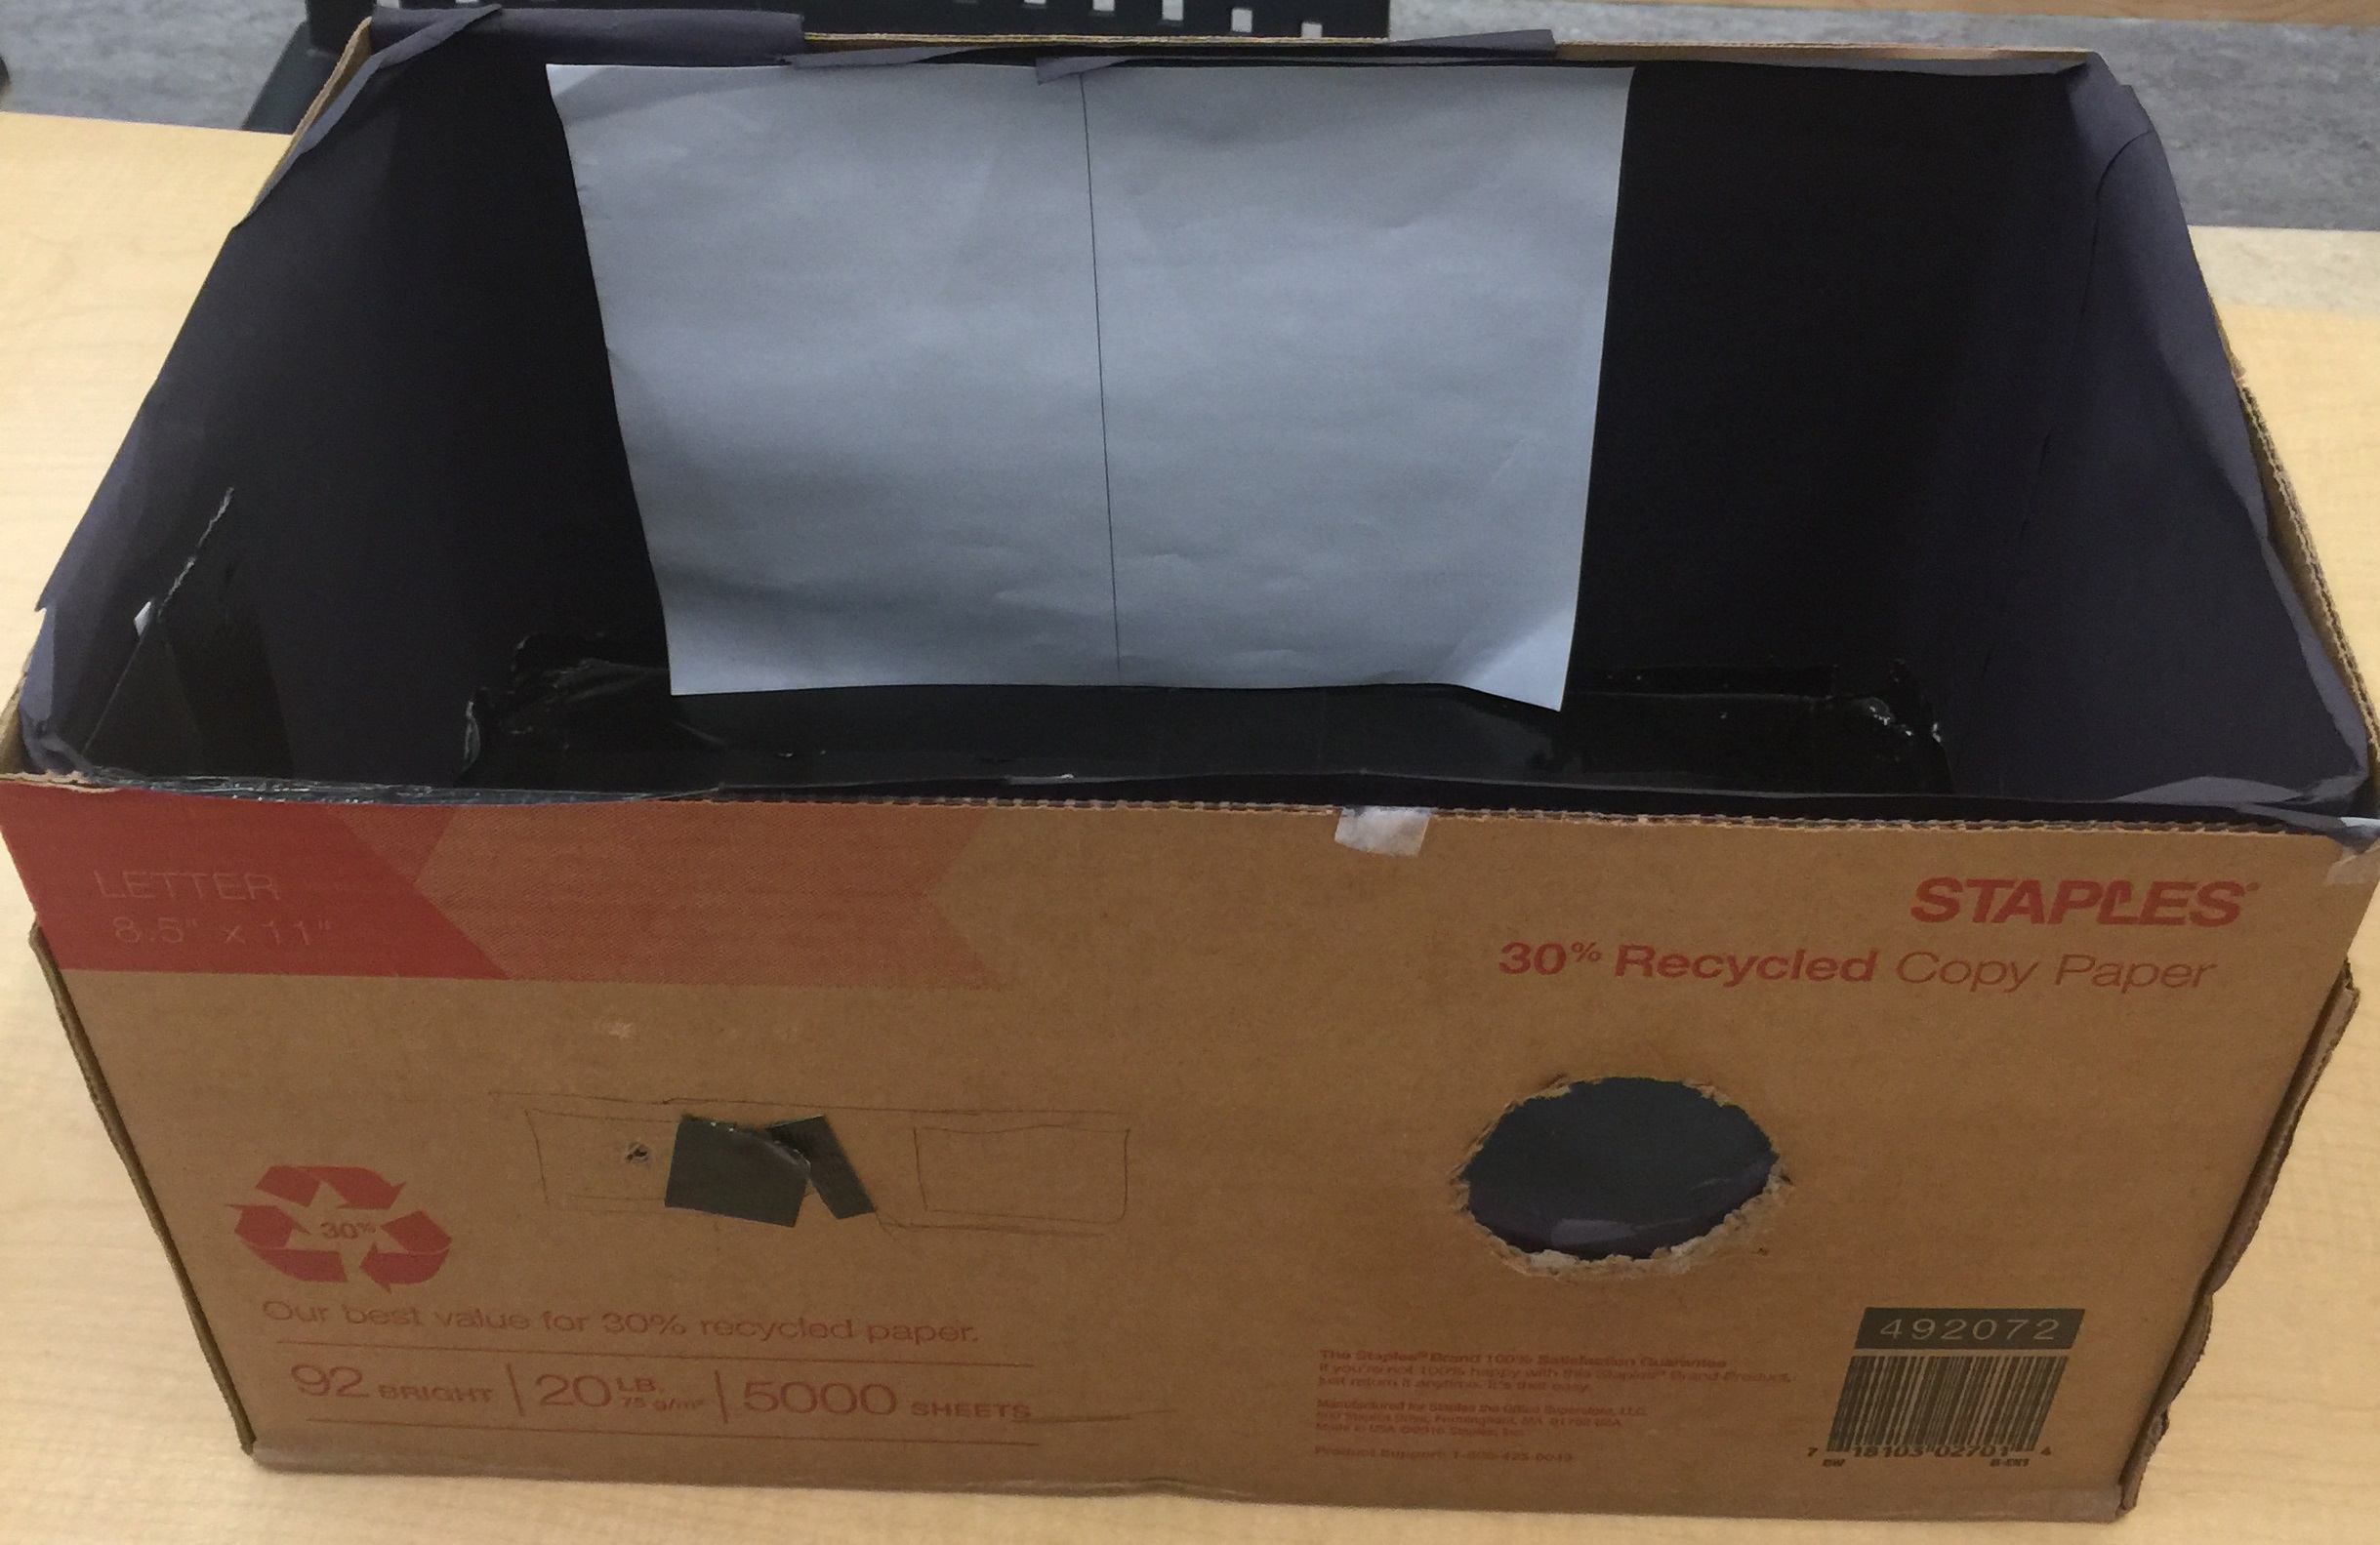
\includegraphics[width=.7\linewidth, height=1in]{IMG_1182.jpg}
		\caption{Camera obscura inside}
	\end{minipage}
	\begin{minipage}[b]{.5\linewidth}
		\centering
		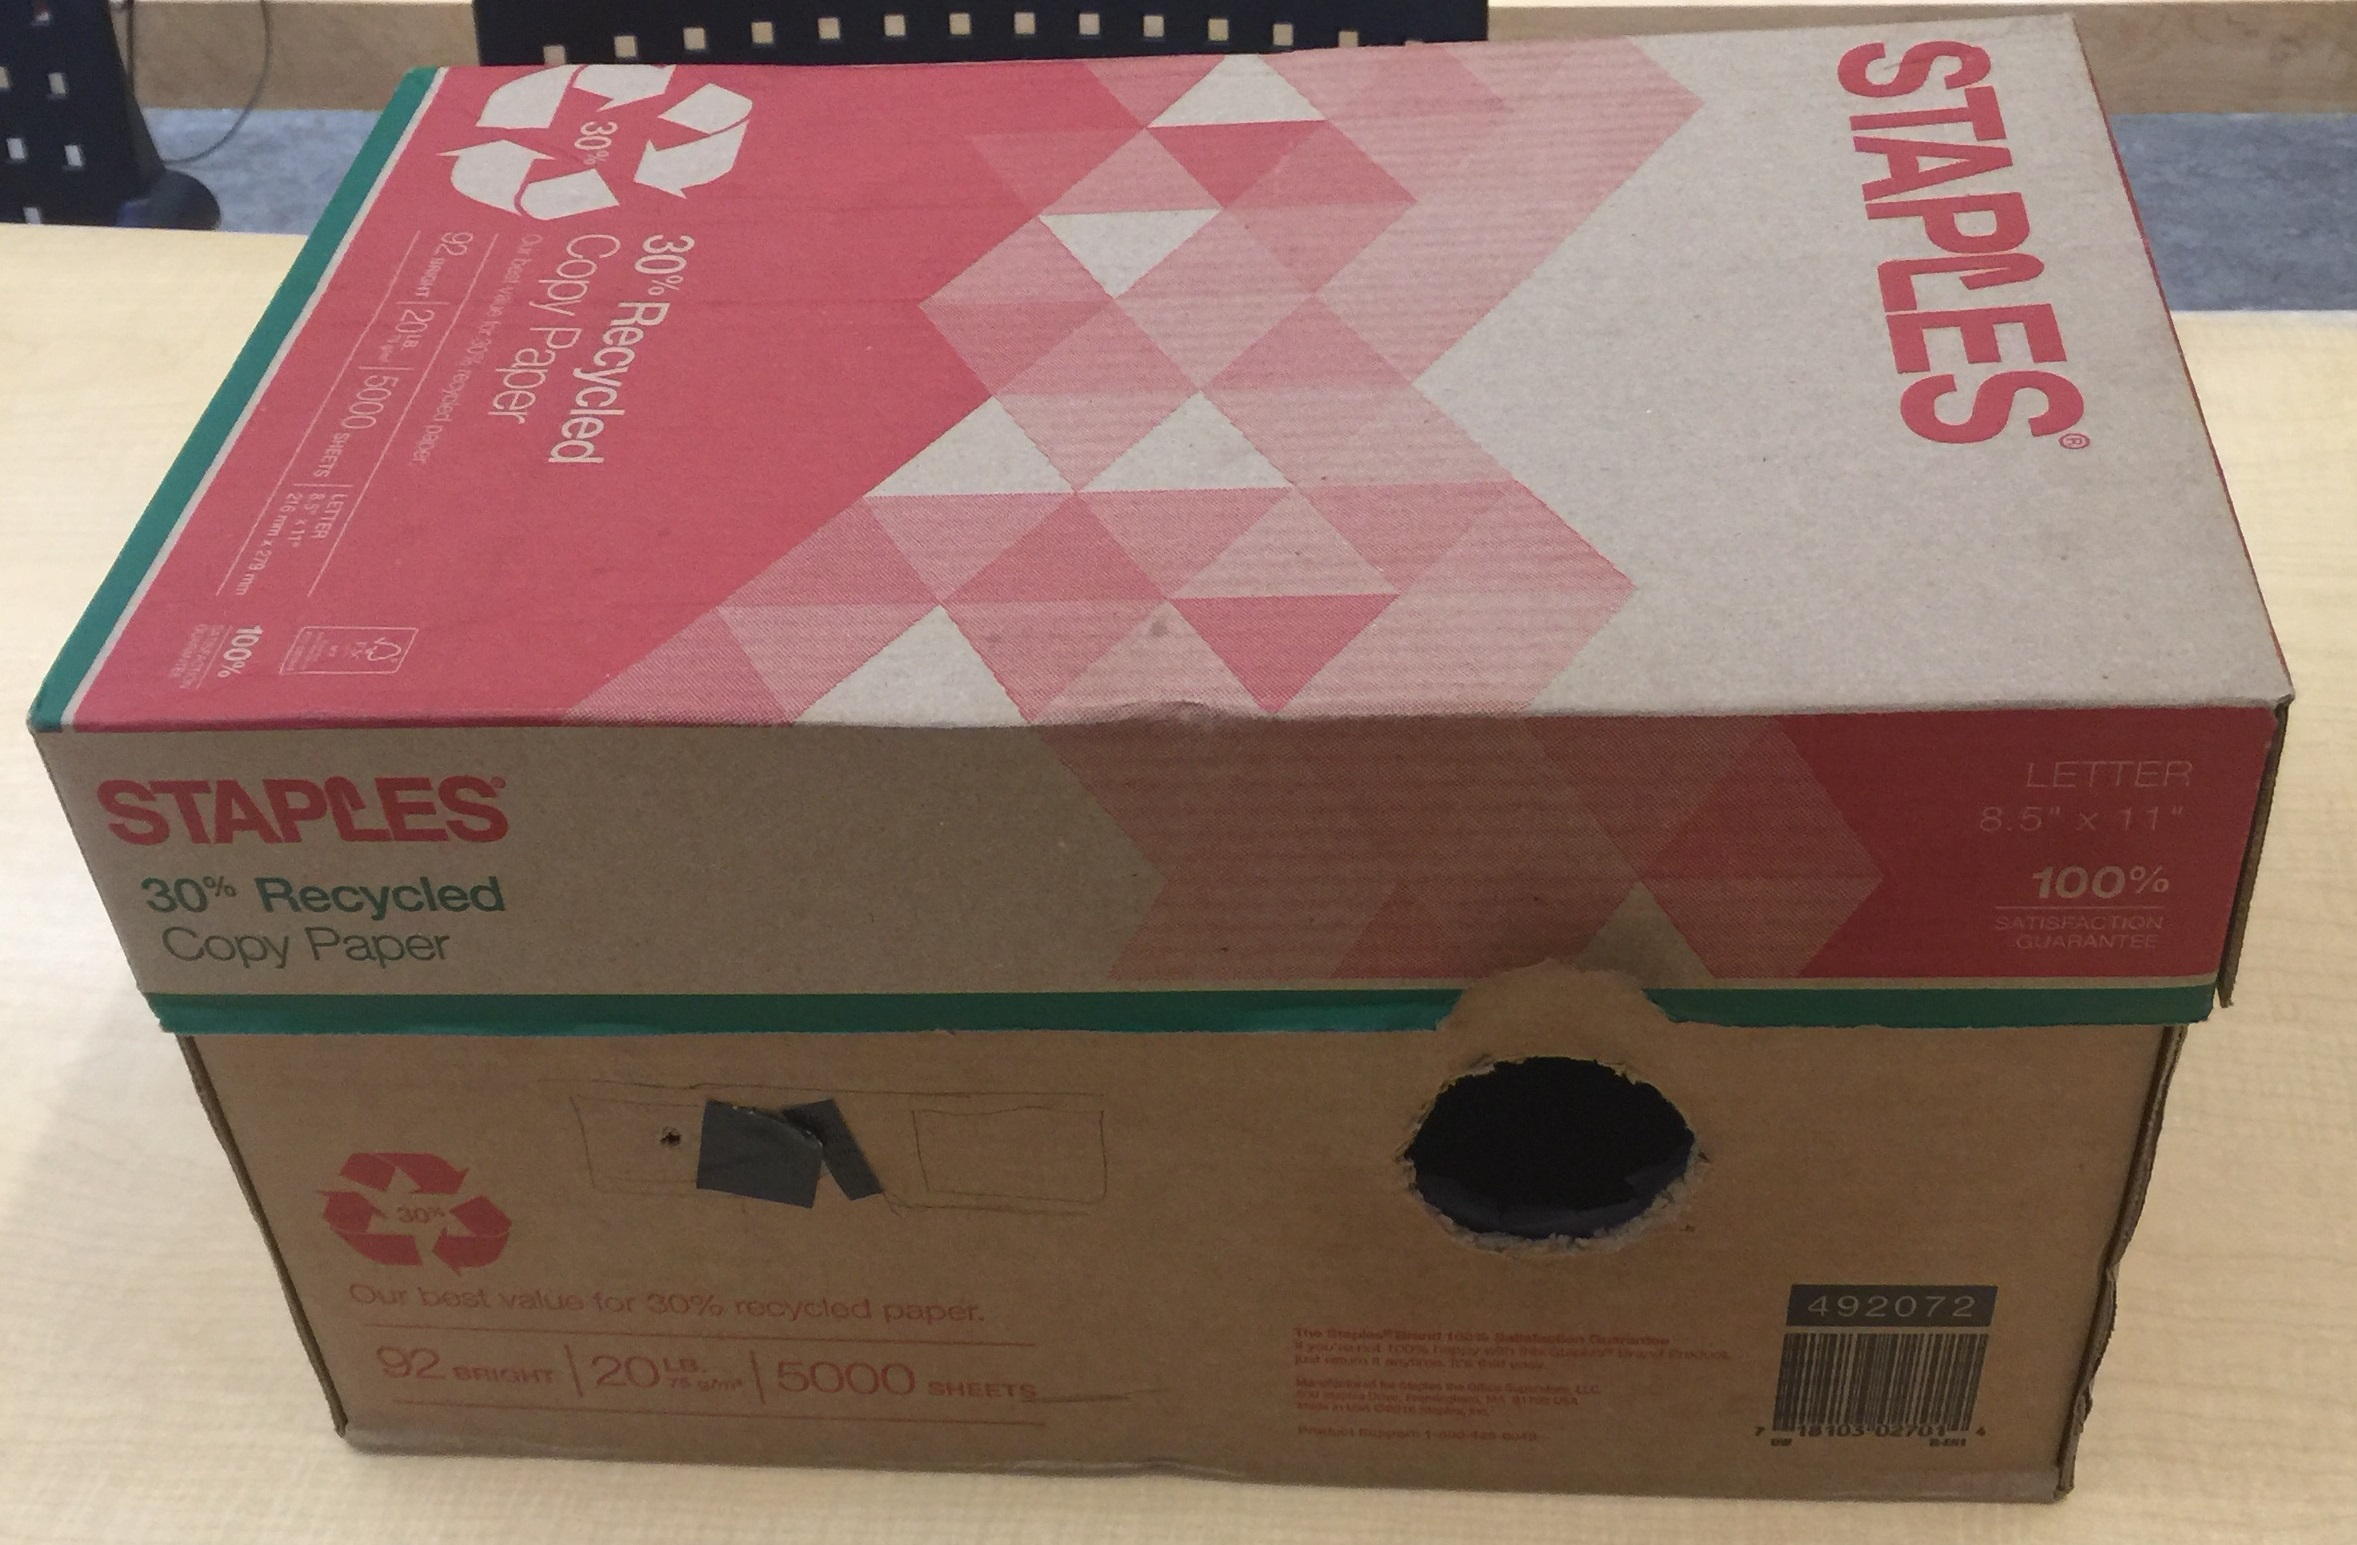
\includegraphics[width=.7\linewidth, height=1in]{IMG_1183.jpg}
		\caption{Camera obscura box}
	\end{minipage}
\end{figure}
\newline 1.2 \emph{Taking a picture with the camera obscura}
\begin{figure}[H]
	\centering
	\begin{minipage}[b]{.5\linewidth}
		\centering
		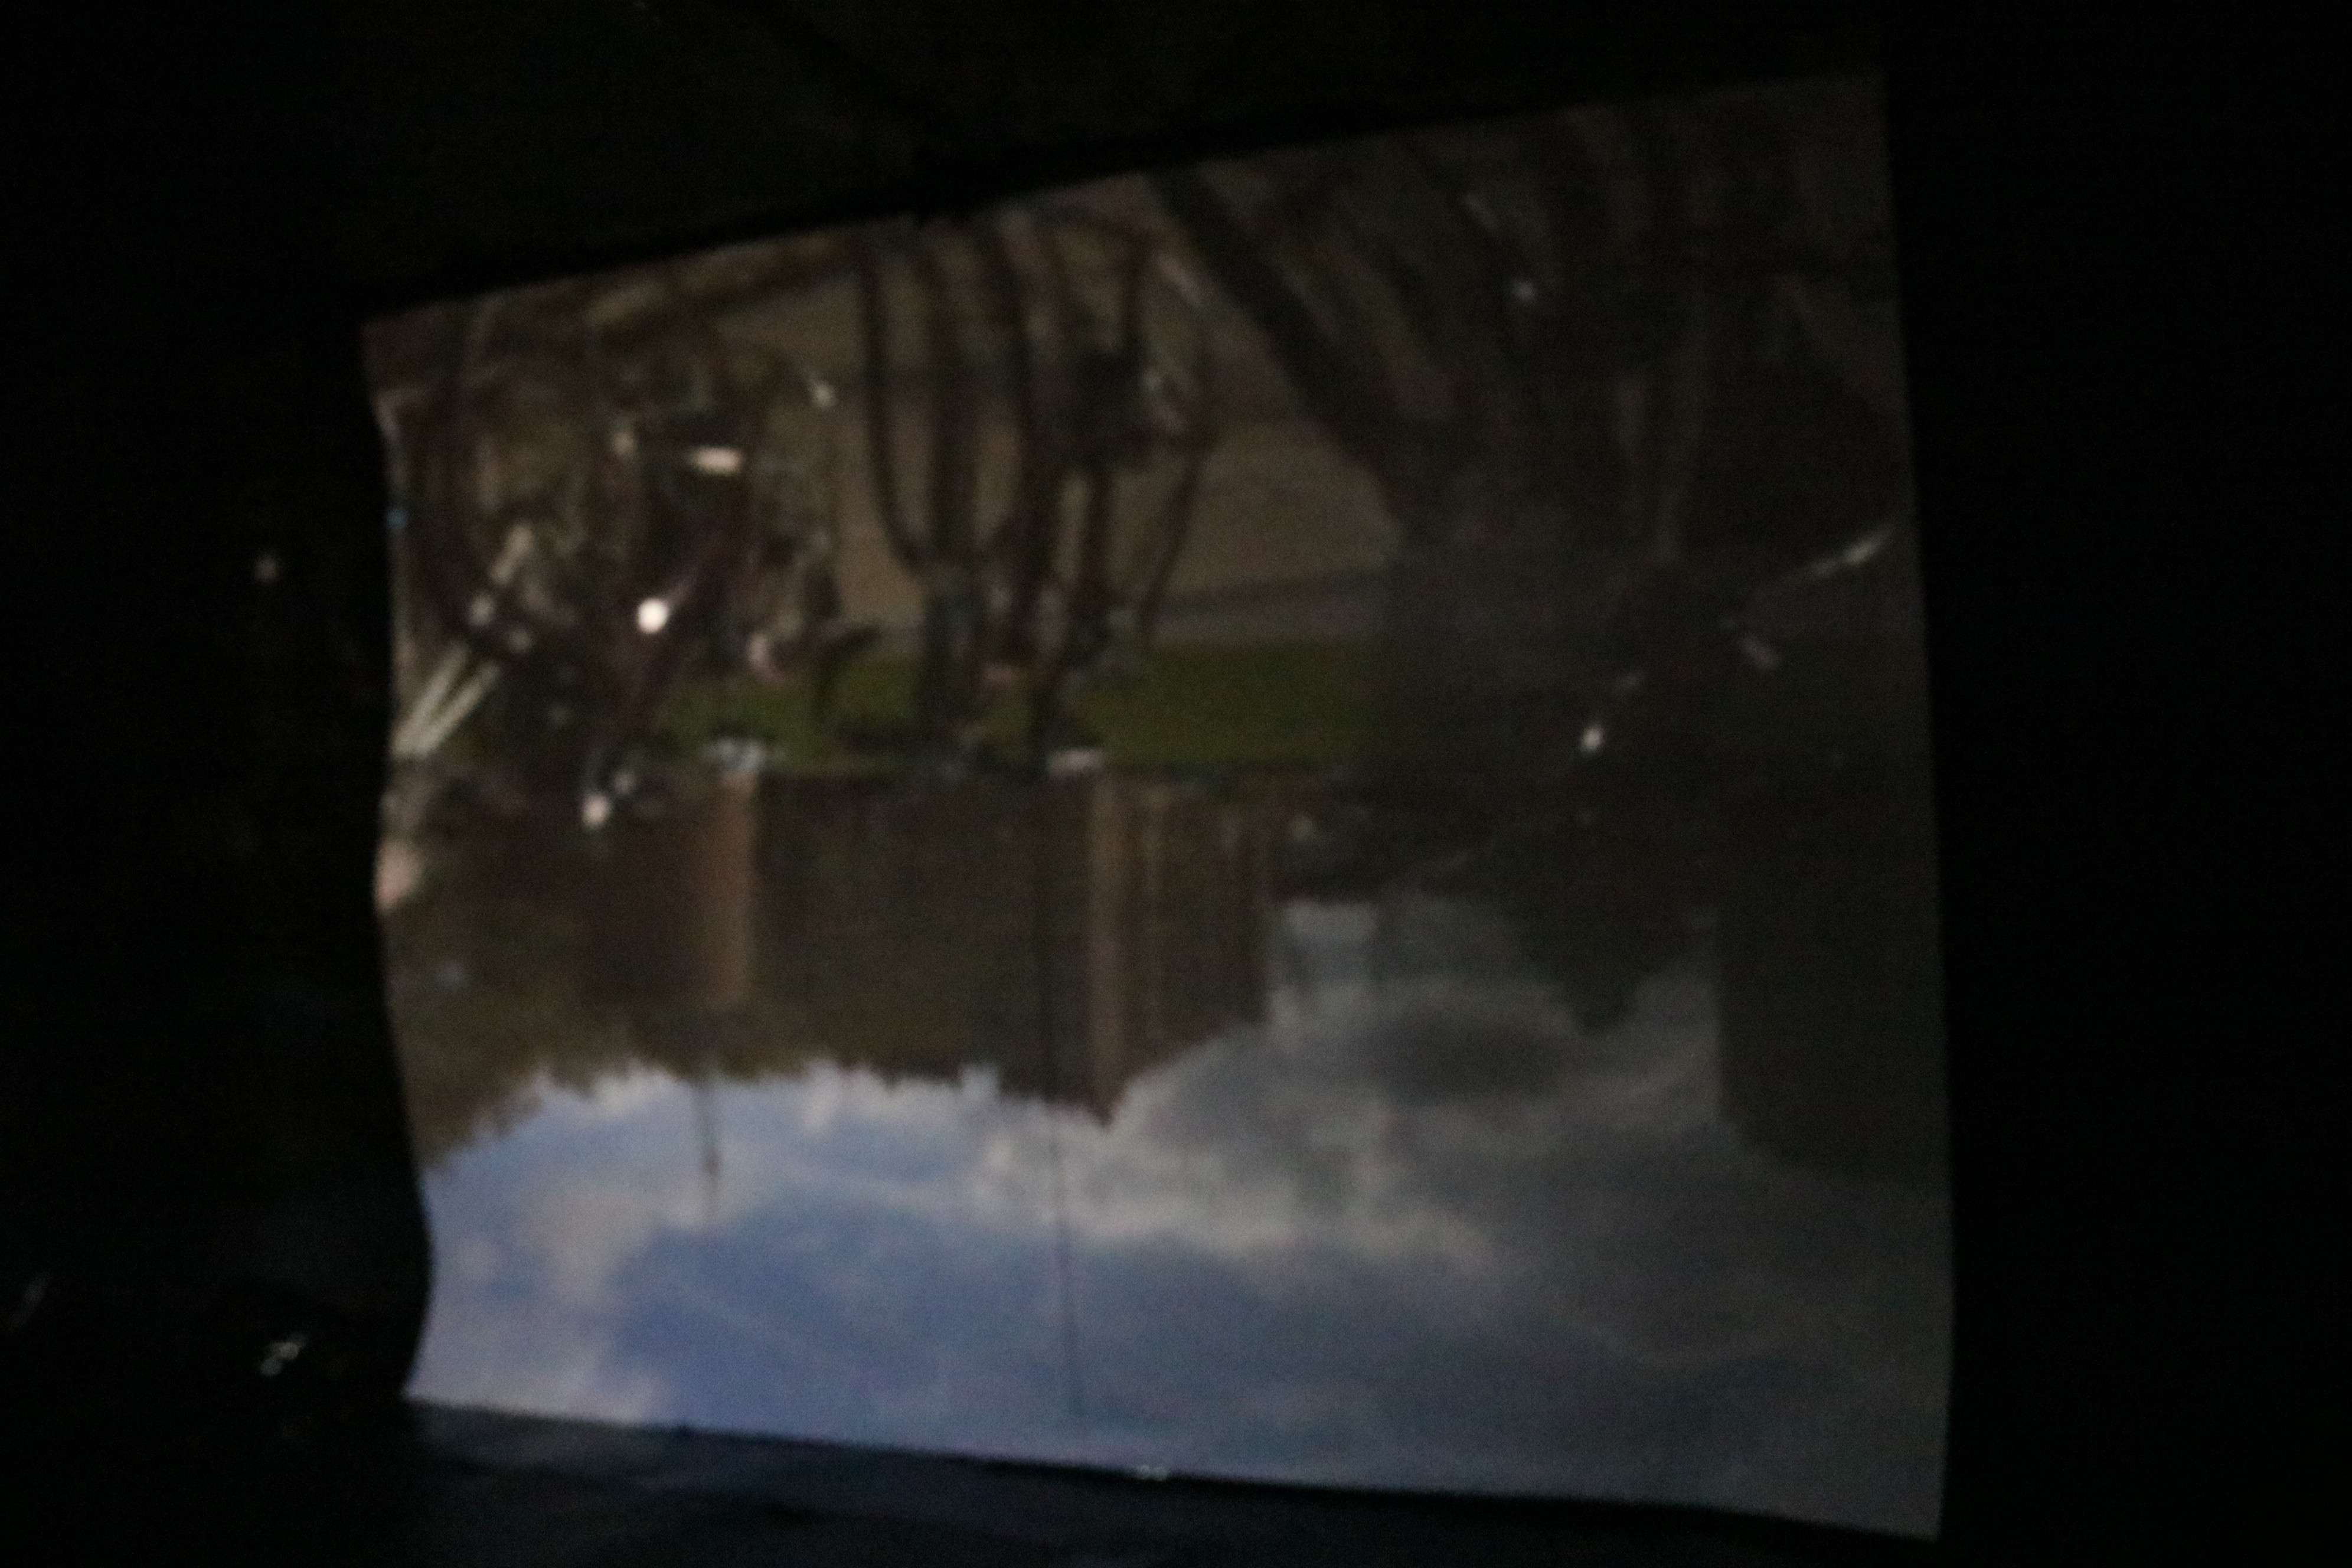
\includegraphics[width=.7\linewidth, height=1in]{IMG_1554.JPG}
		\caption{Scene 1}
	\end{minipage}
	\begin{minipage}[b]{.5\linewidth}
		\centering
		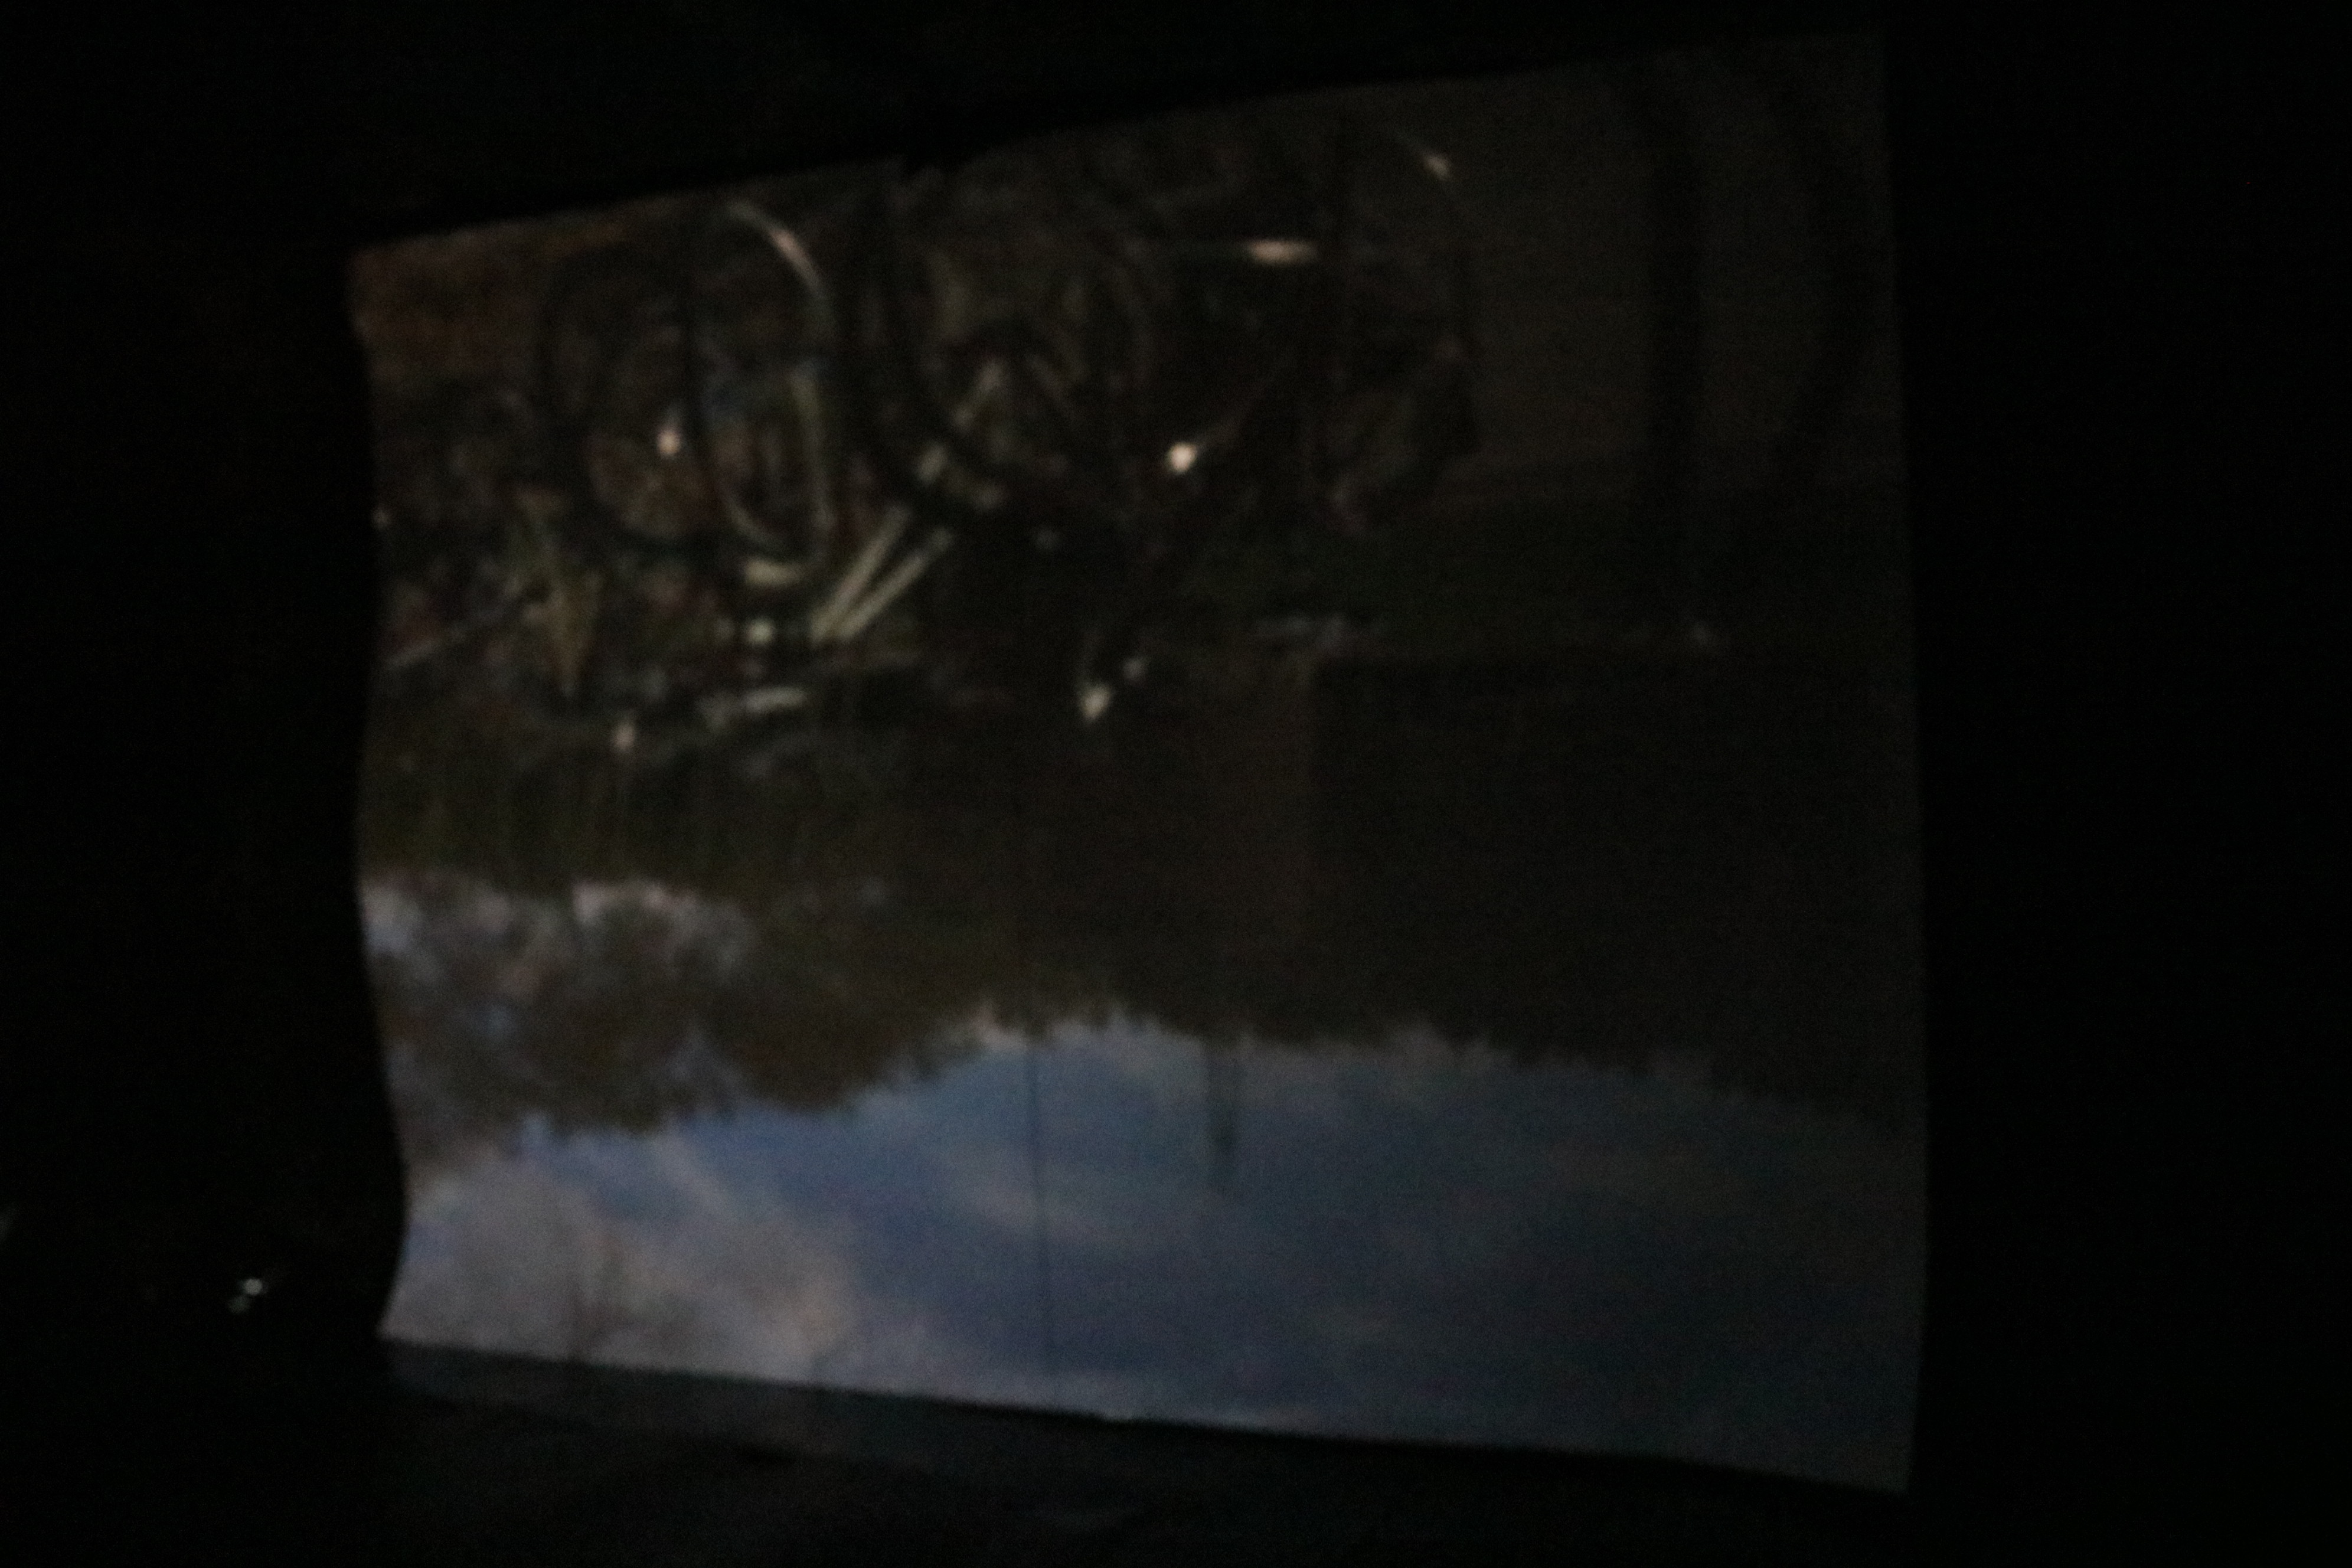
\includegraphics[width=.7\linewidth, height=1in]{IMG_1582.JPG}
		\caption{Scene 2}
	\end{minipage}
	\begin{minipage}[b]{.5\linewidth}
		\centering
		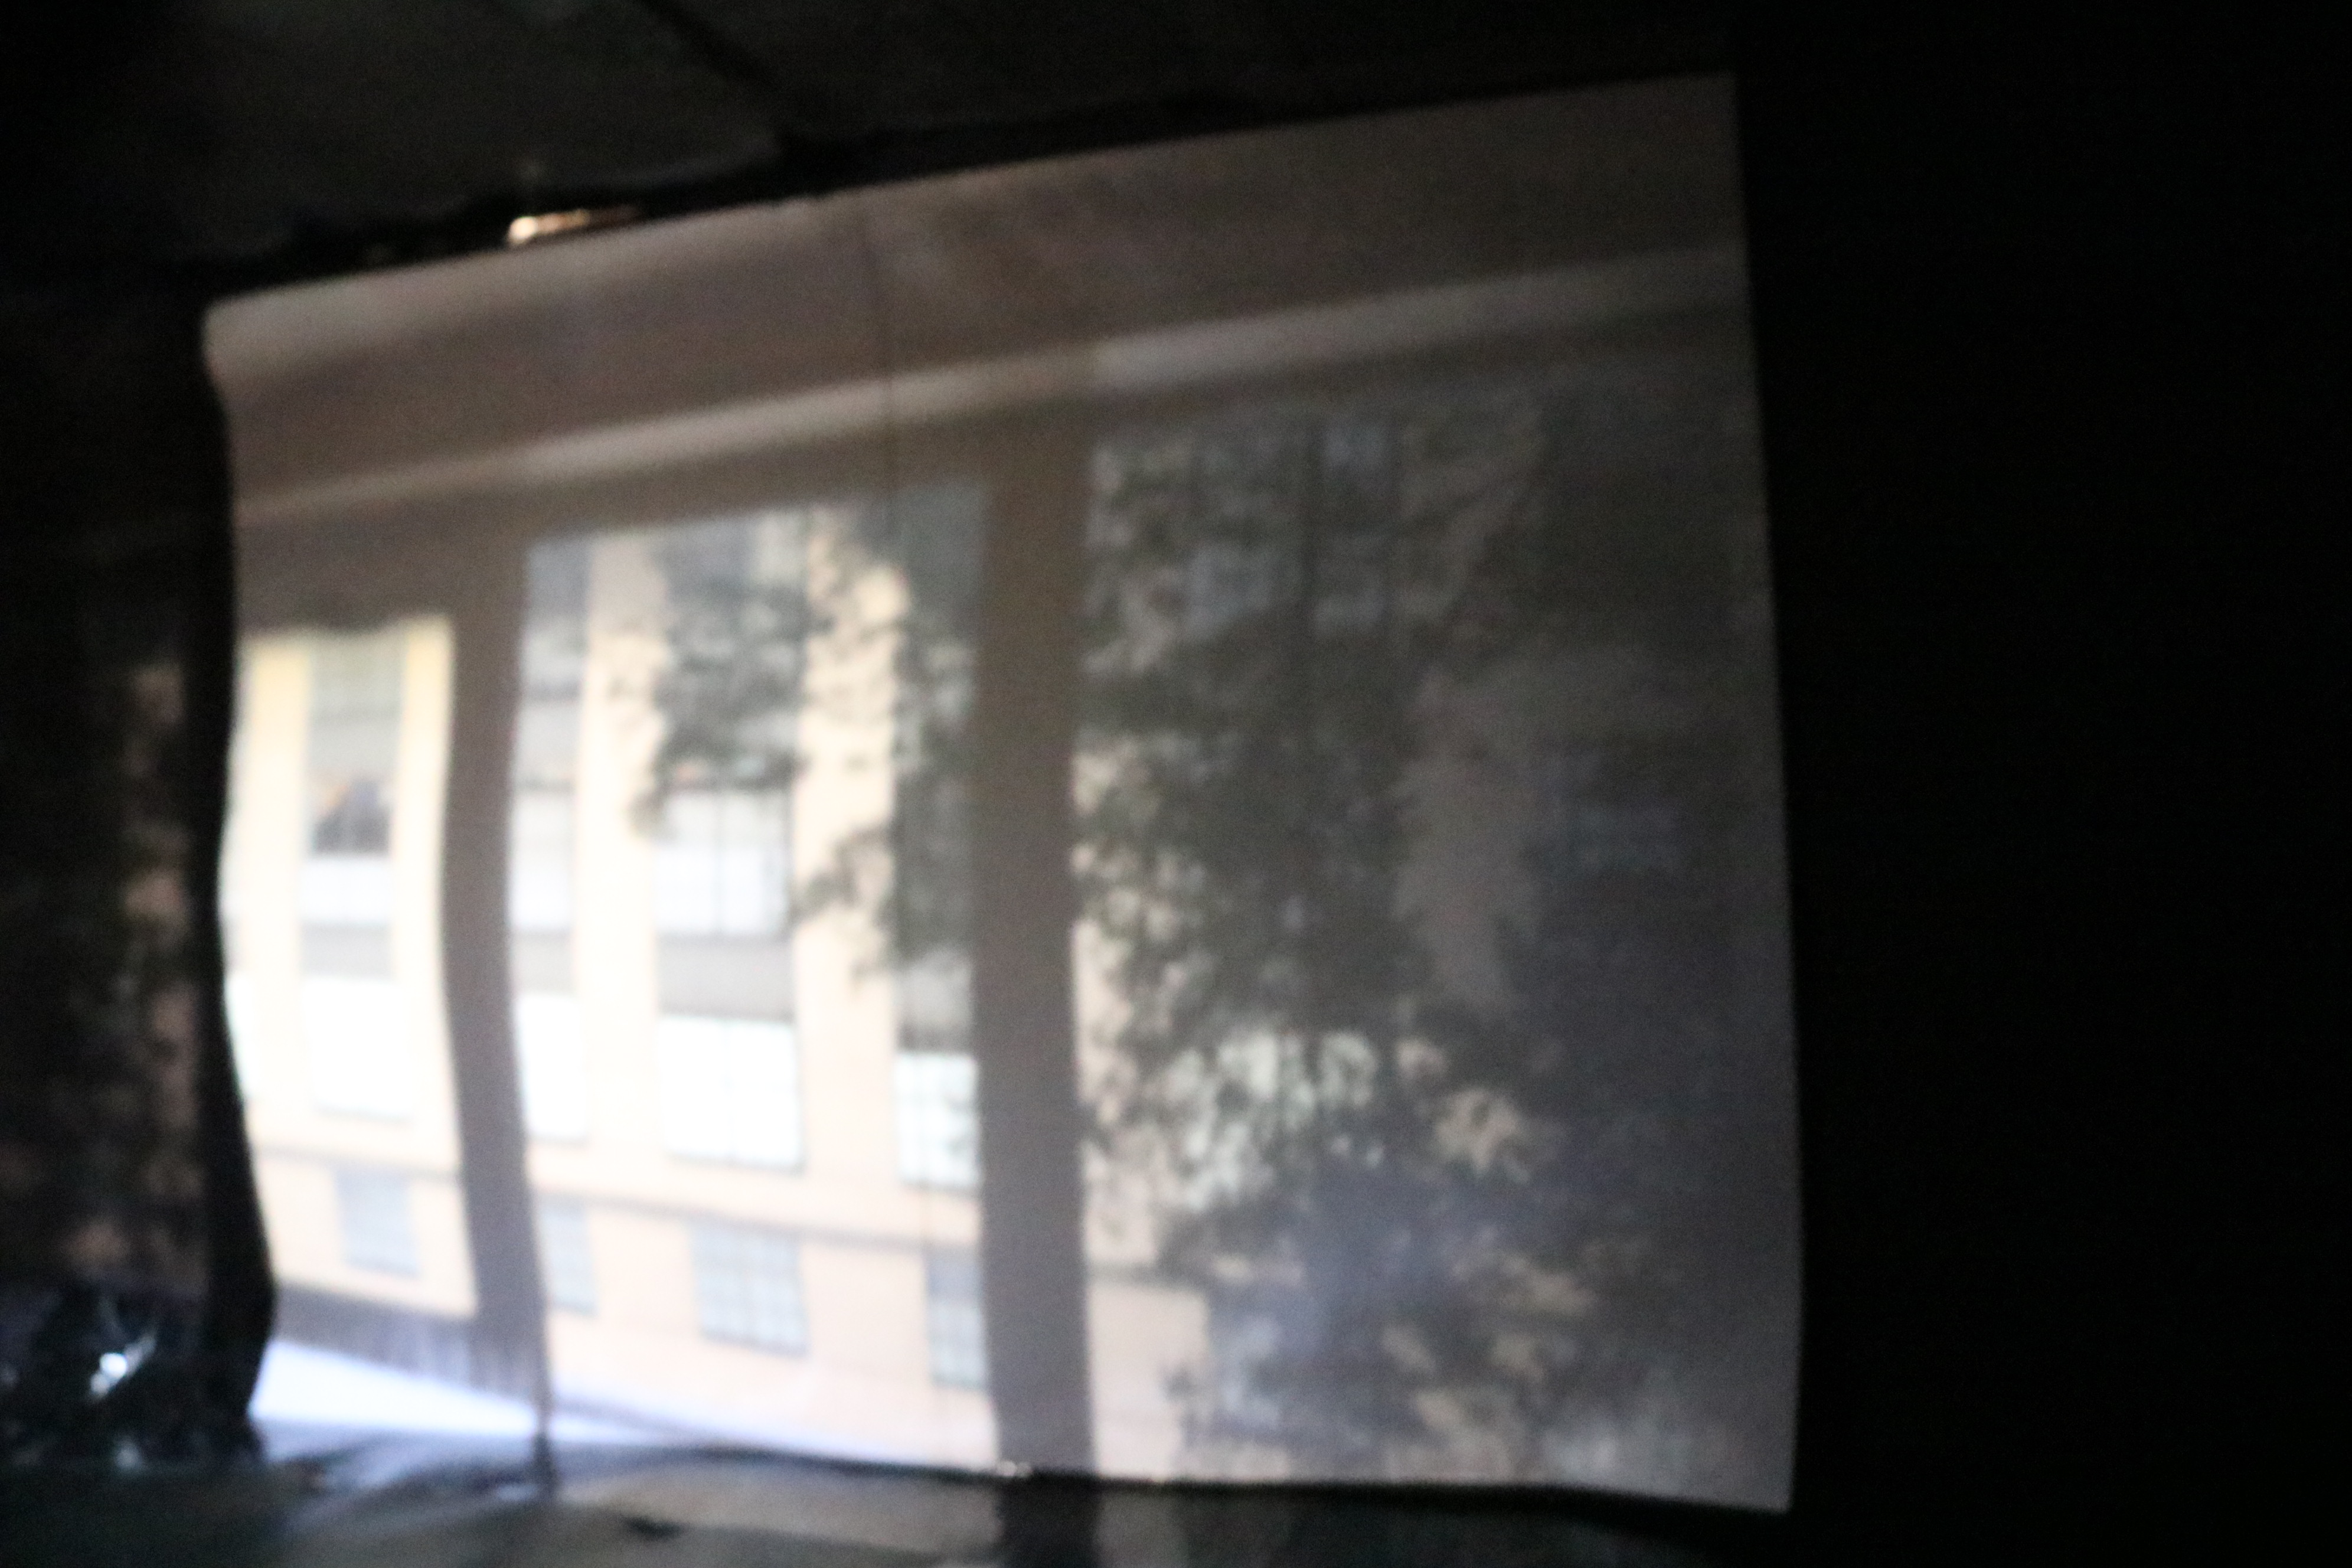
\includegraphics[width=.7\linewidth, height=1in]{IMG_1591.JPG}
		\caption{Scene 3}
	\end{minipage}
	\begin{minipage}[b]{.5\linewidth}
		\centering
		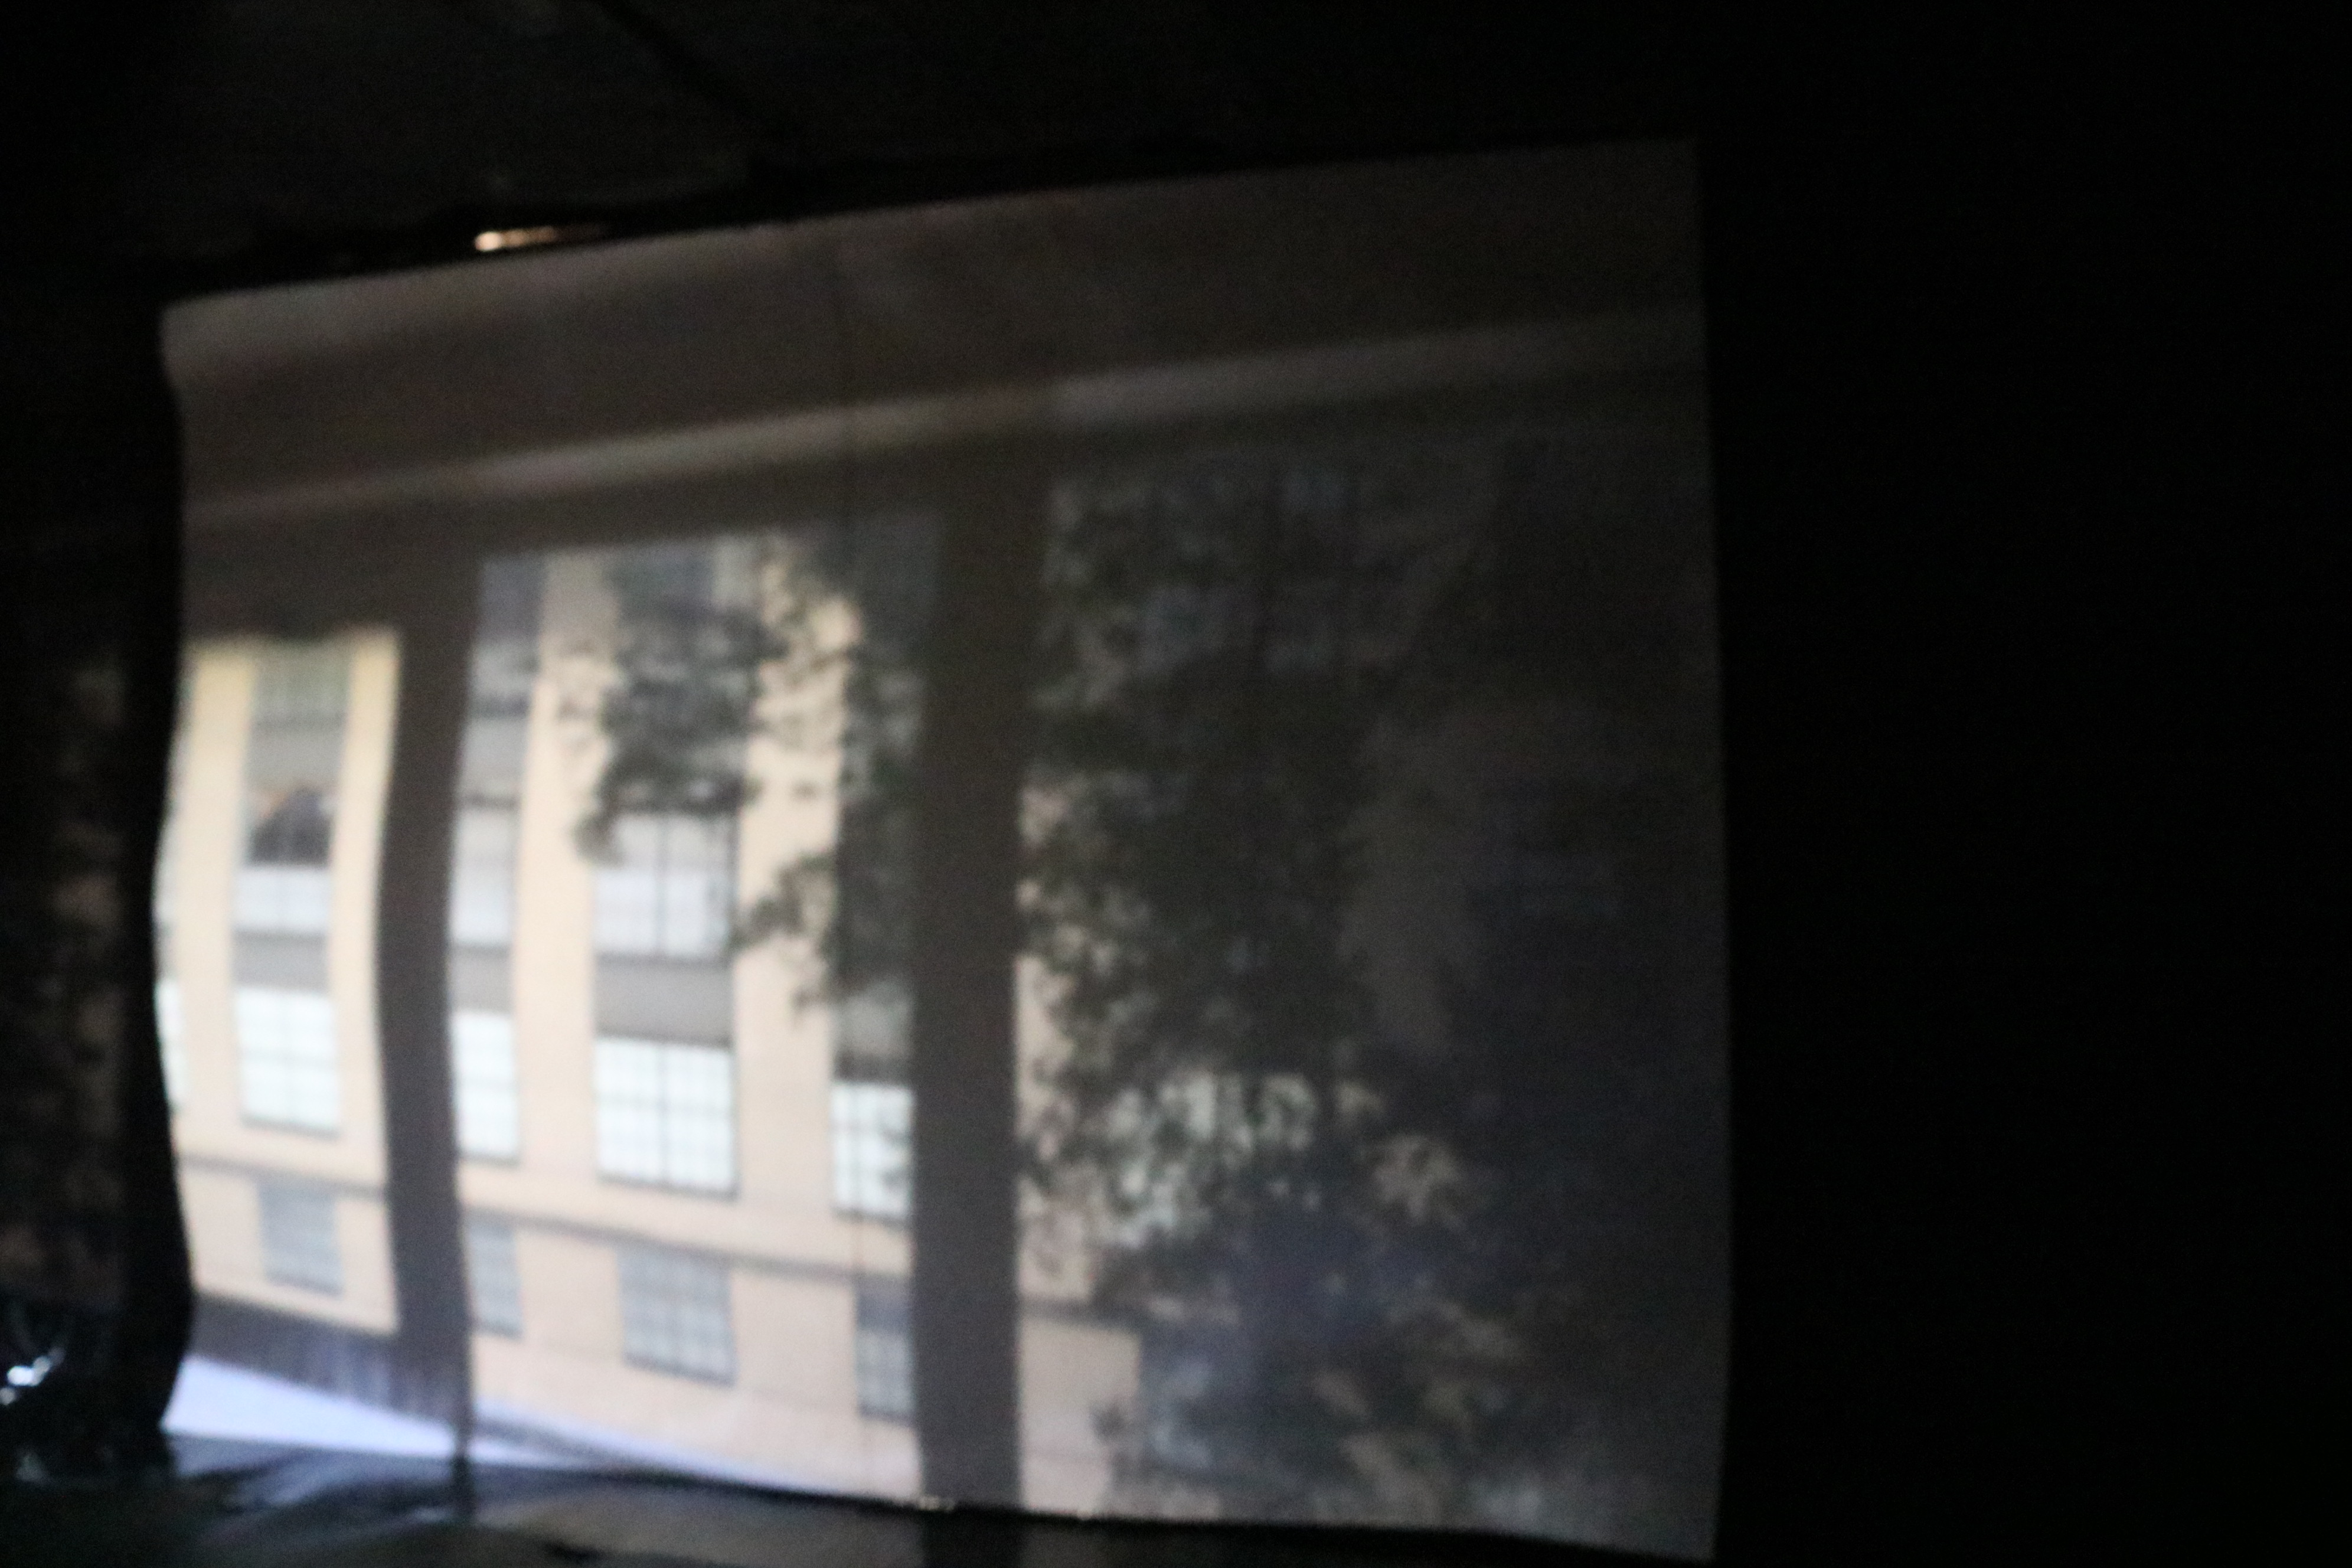
\includegraphics[width=.7\linewidth, height=1in]{IMG_1593.JPG}
		\caption{Scene 4}
	\end{minipage}
	\begin{minipage}[b]{.5\linewidth}
		\centering
		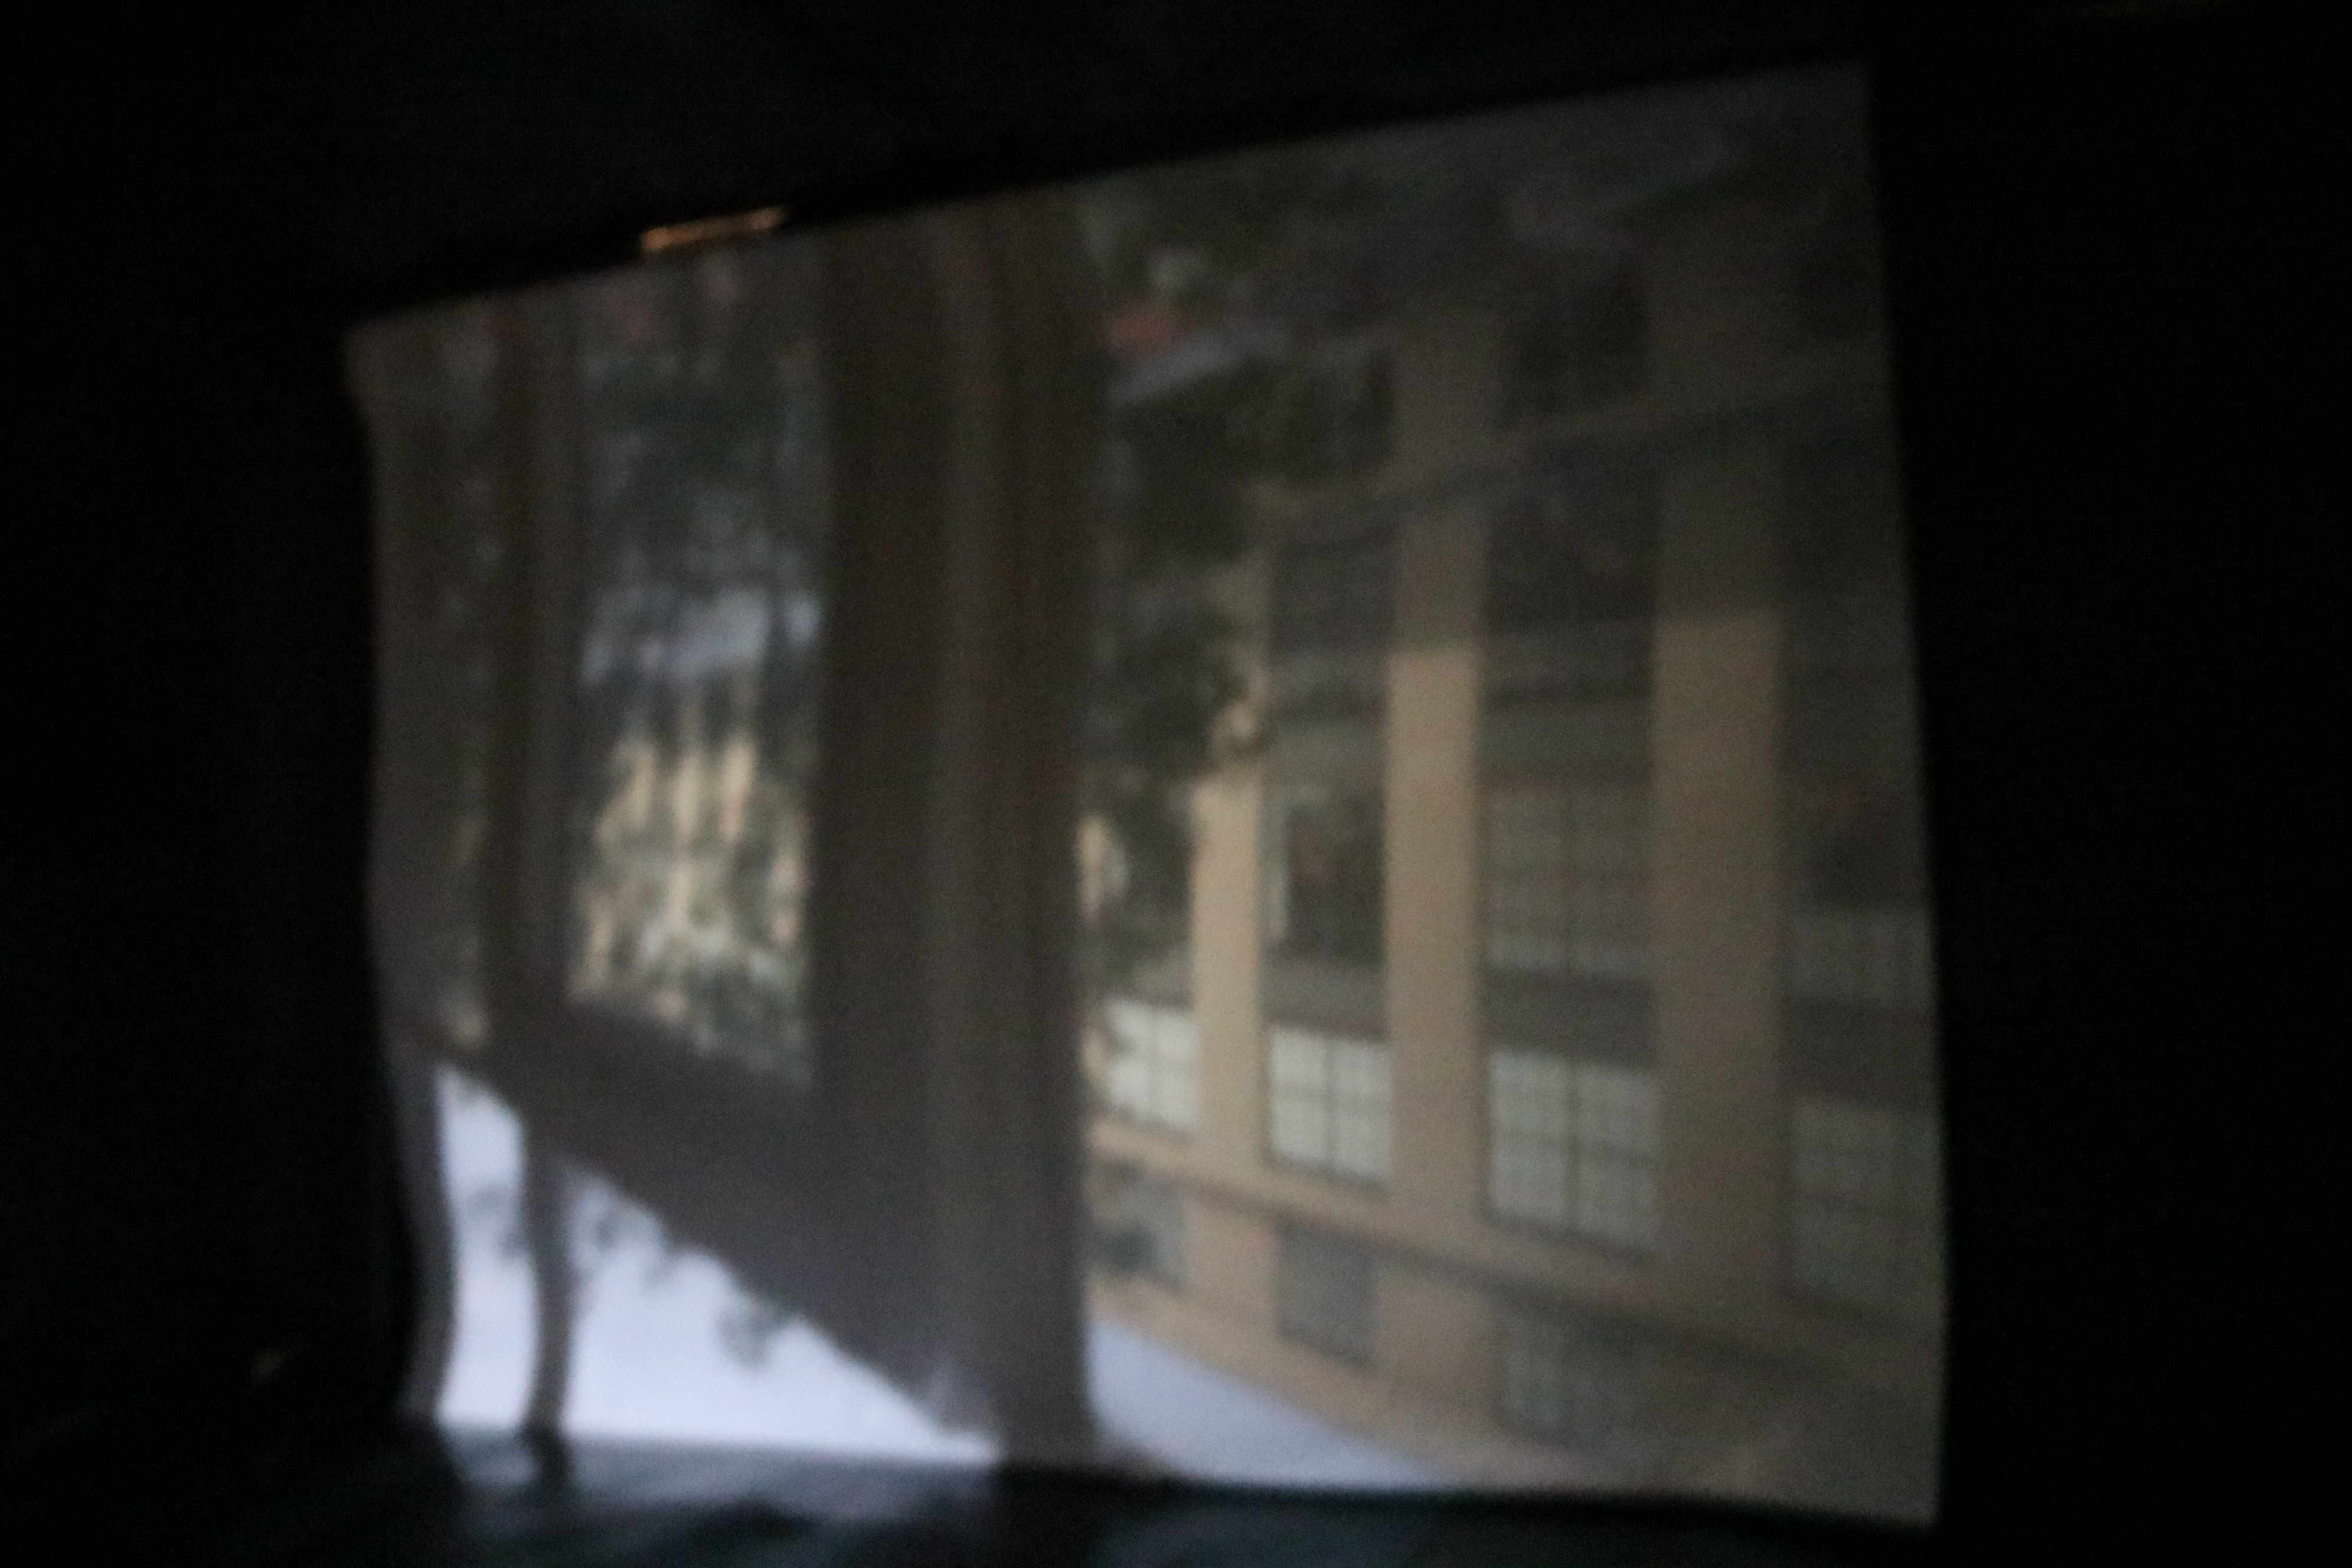
\includegraphics[width=.7\linewidth, height=1in]{IMG_1599.JPG}
		\caption{Scene 5}
	\end{minipage}
	\end{figure}
\newline \emph{\textbf{2. Anaglyph Camera Obscura}}
%\begin{document}
\newline \emph{3d scenes}
	\begin{figure}[H]
	\centering
	\begin{minipage}[b]{.5\linewidth}
		\centering
		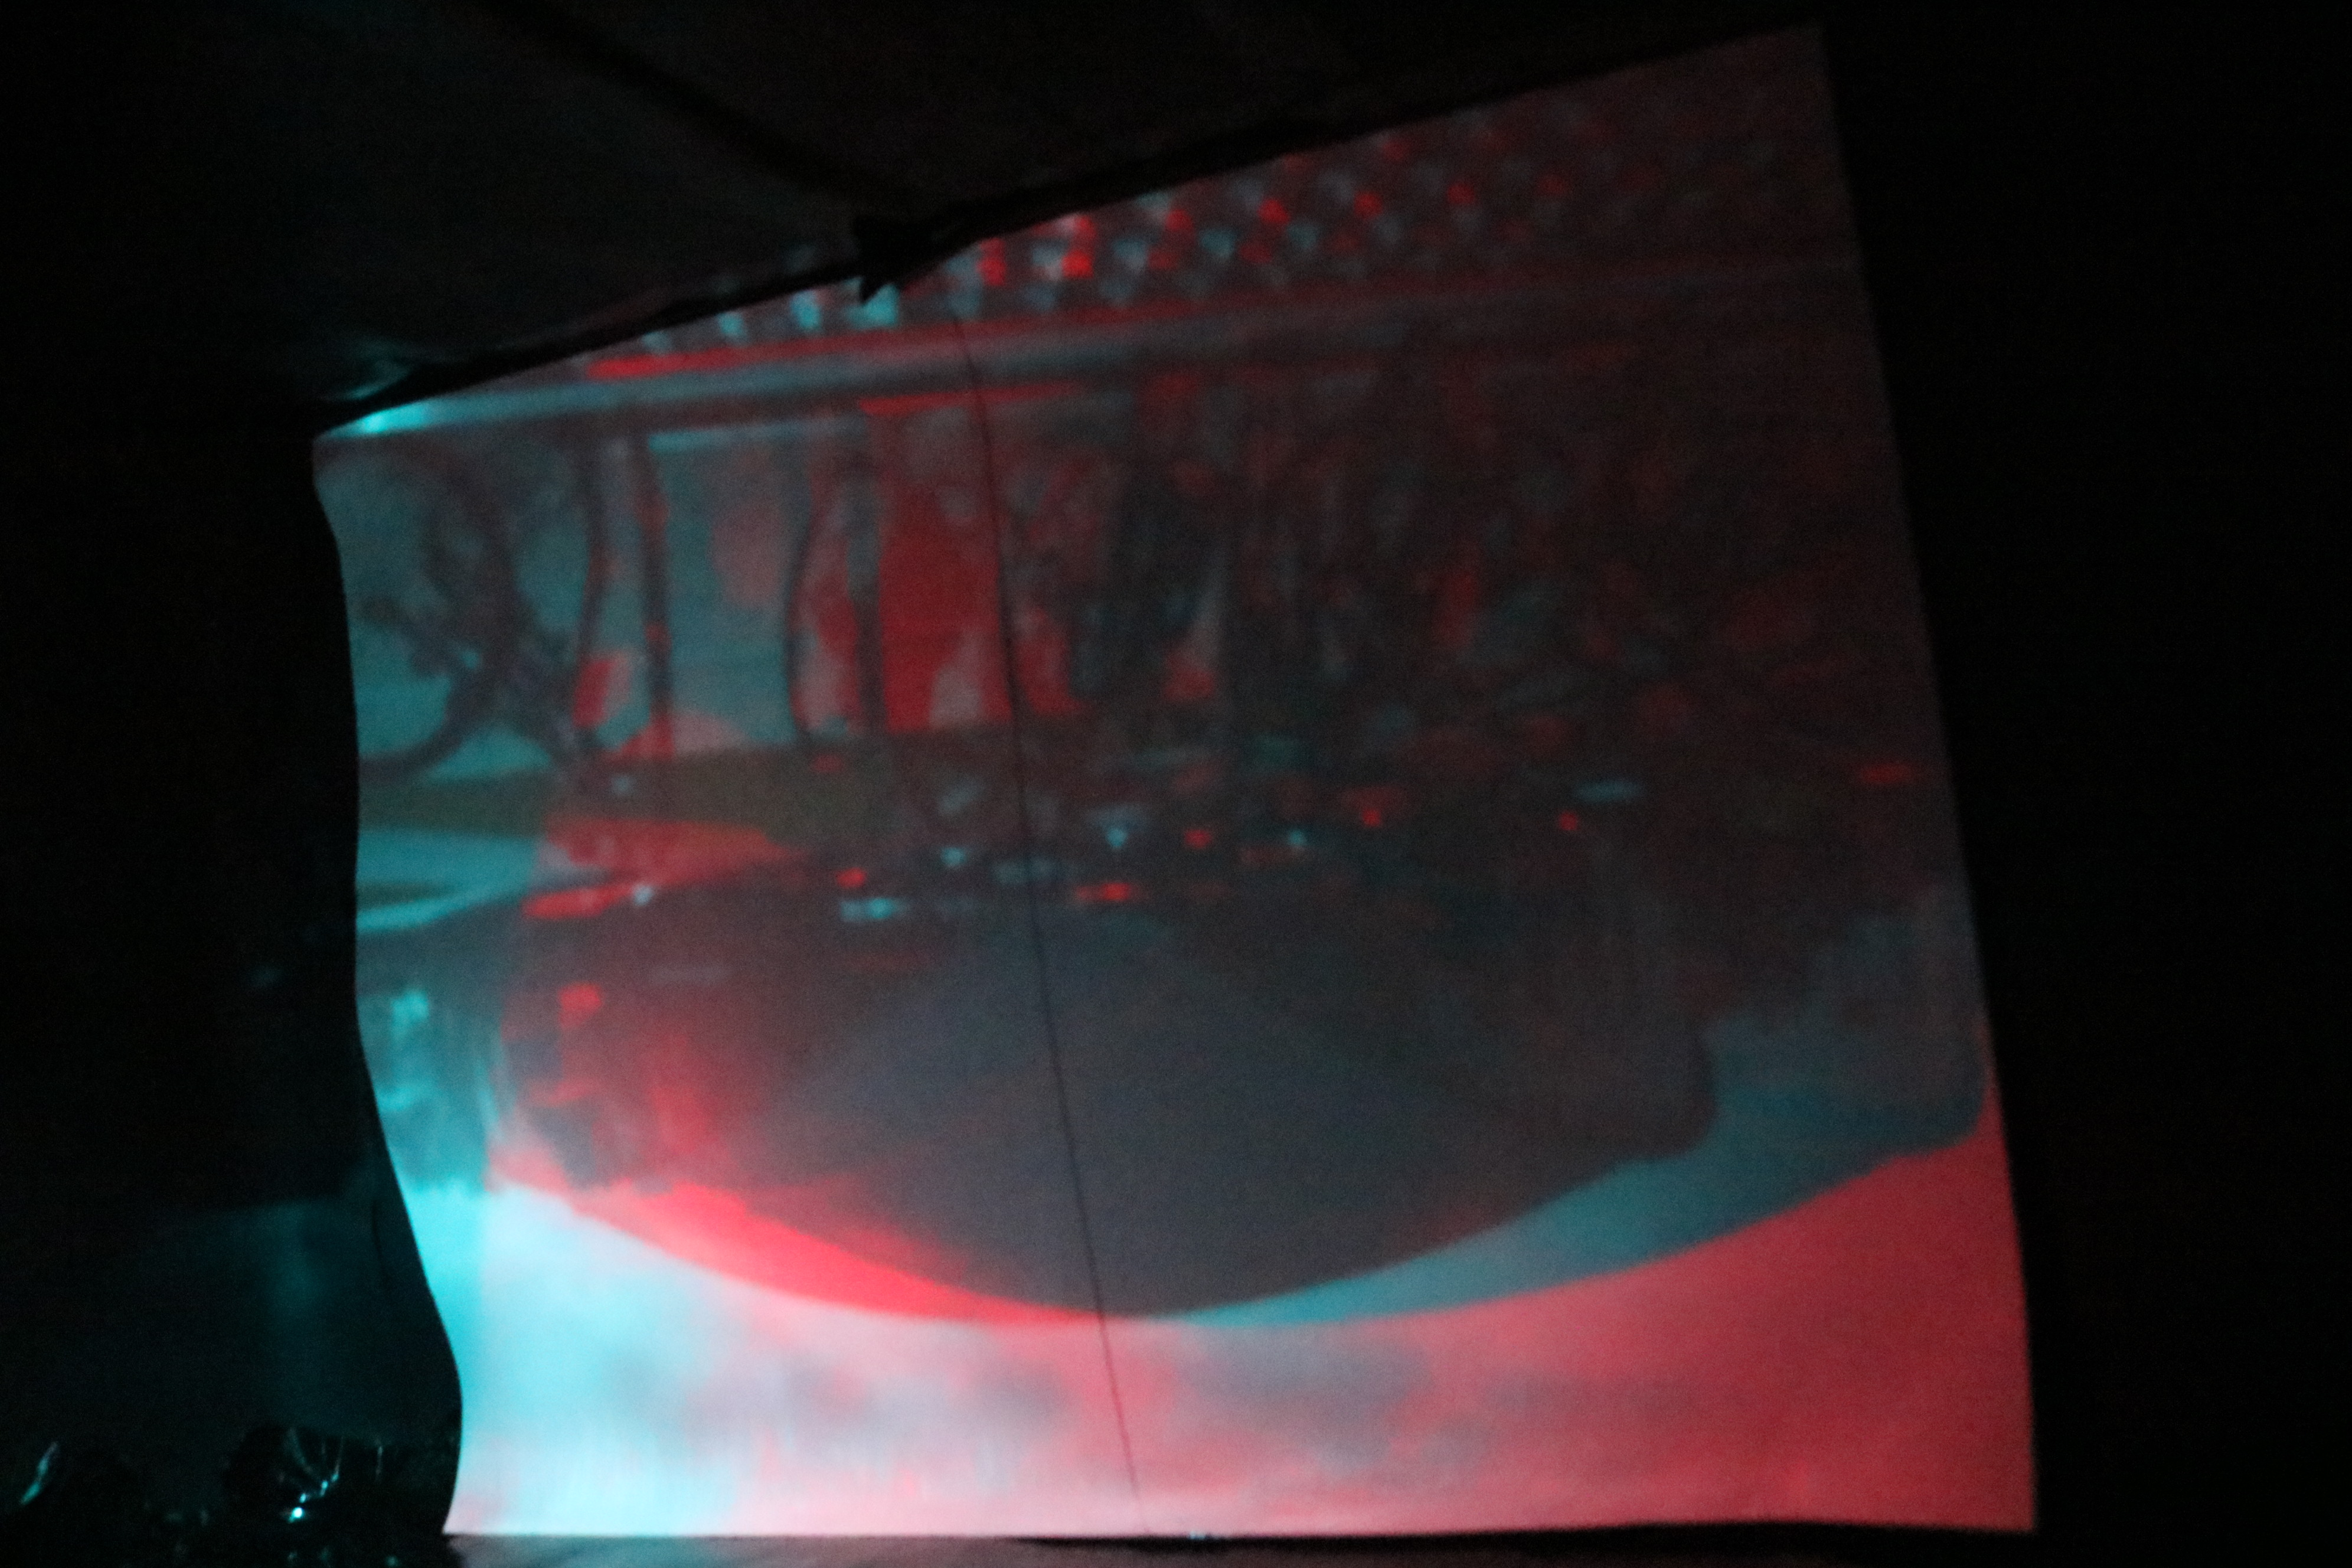
\includegraphics[width=.7\linewidth, height=1in]{IMG_1493.JPG}
		\caption{Scene 1}
	\end{minipage}
	\begin{minipage}[b]{.5\linewidth}
		\centering
		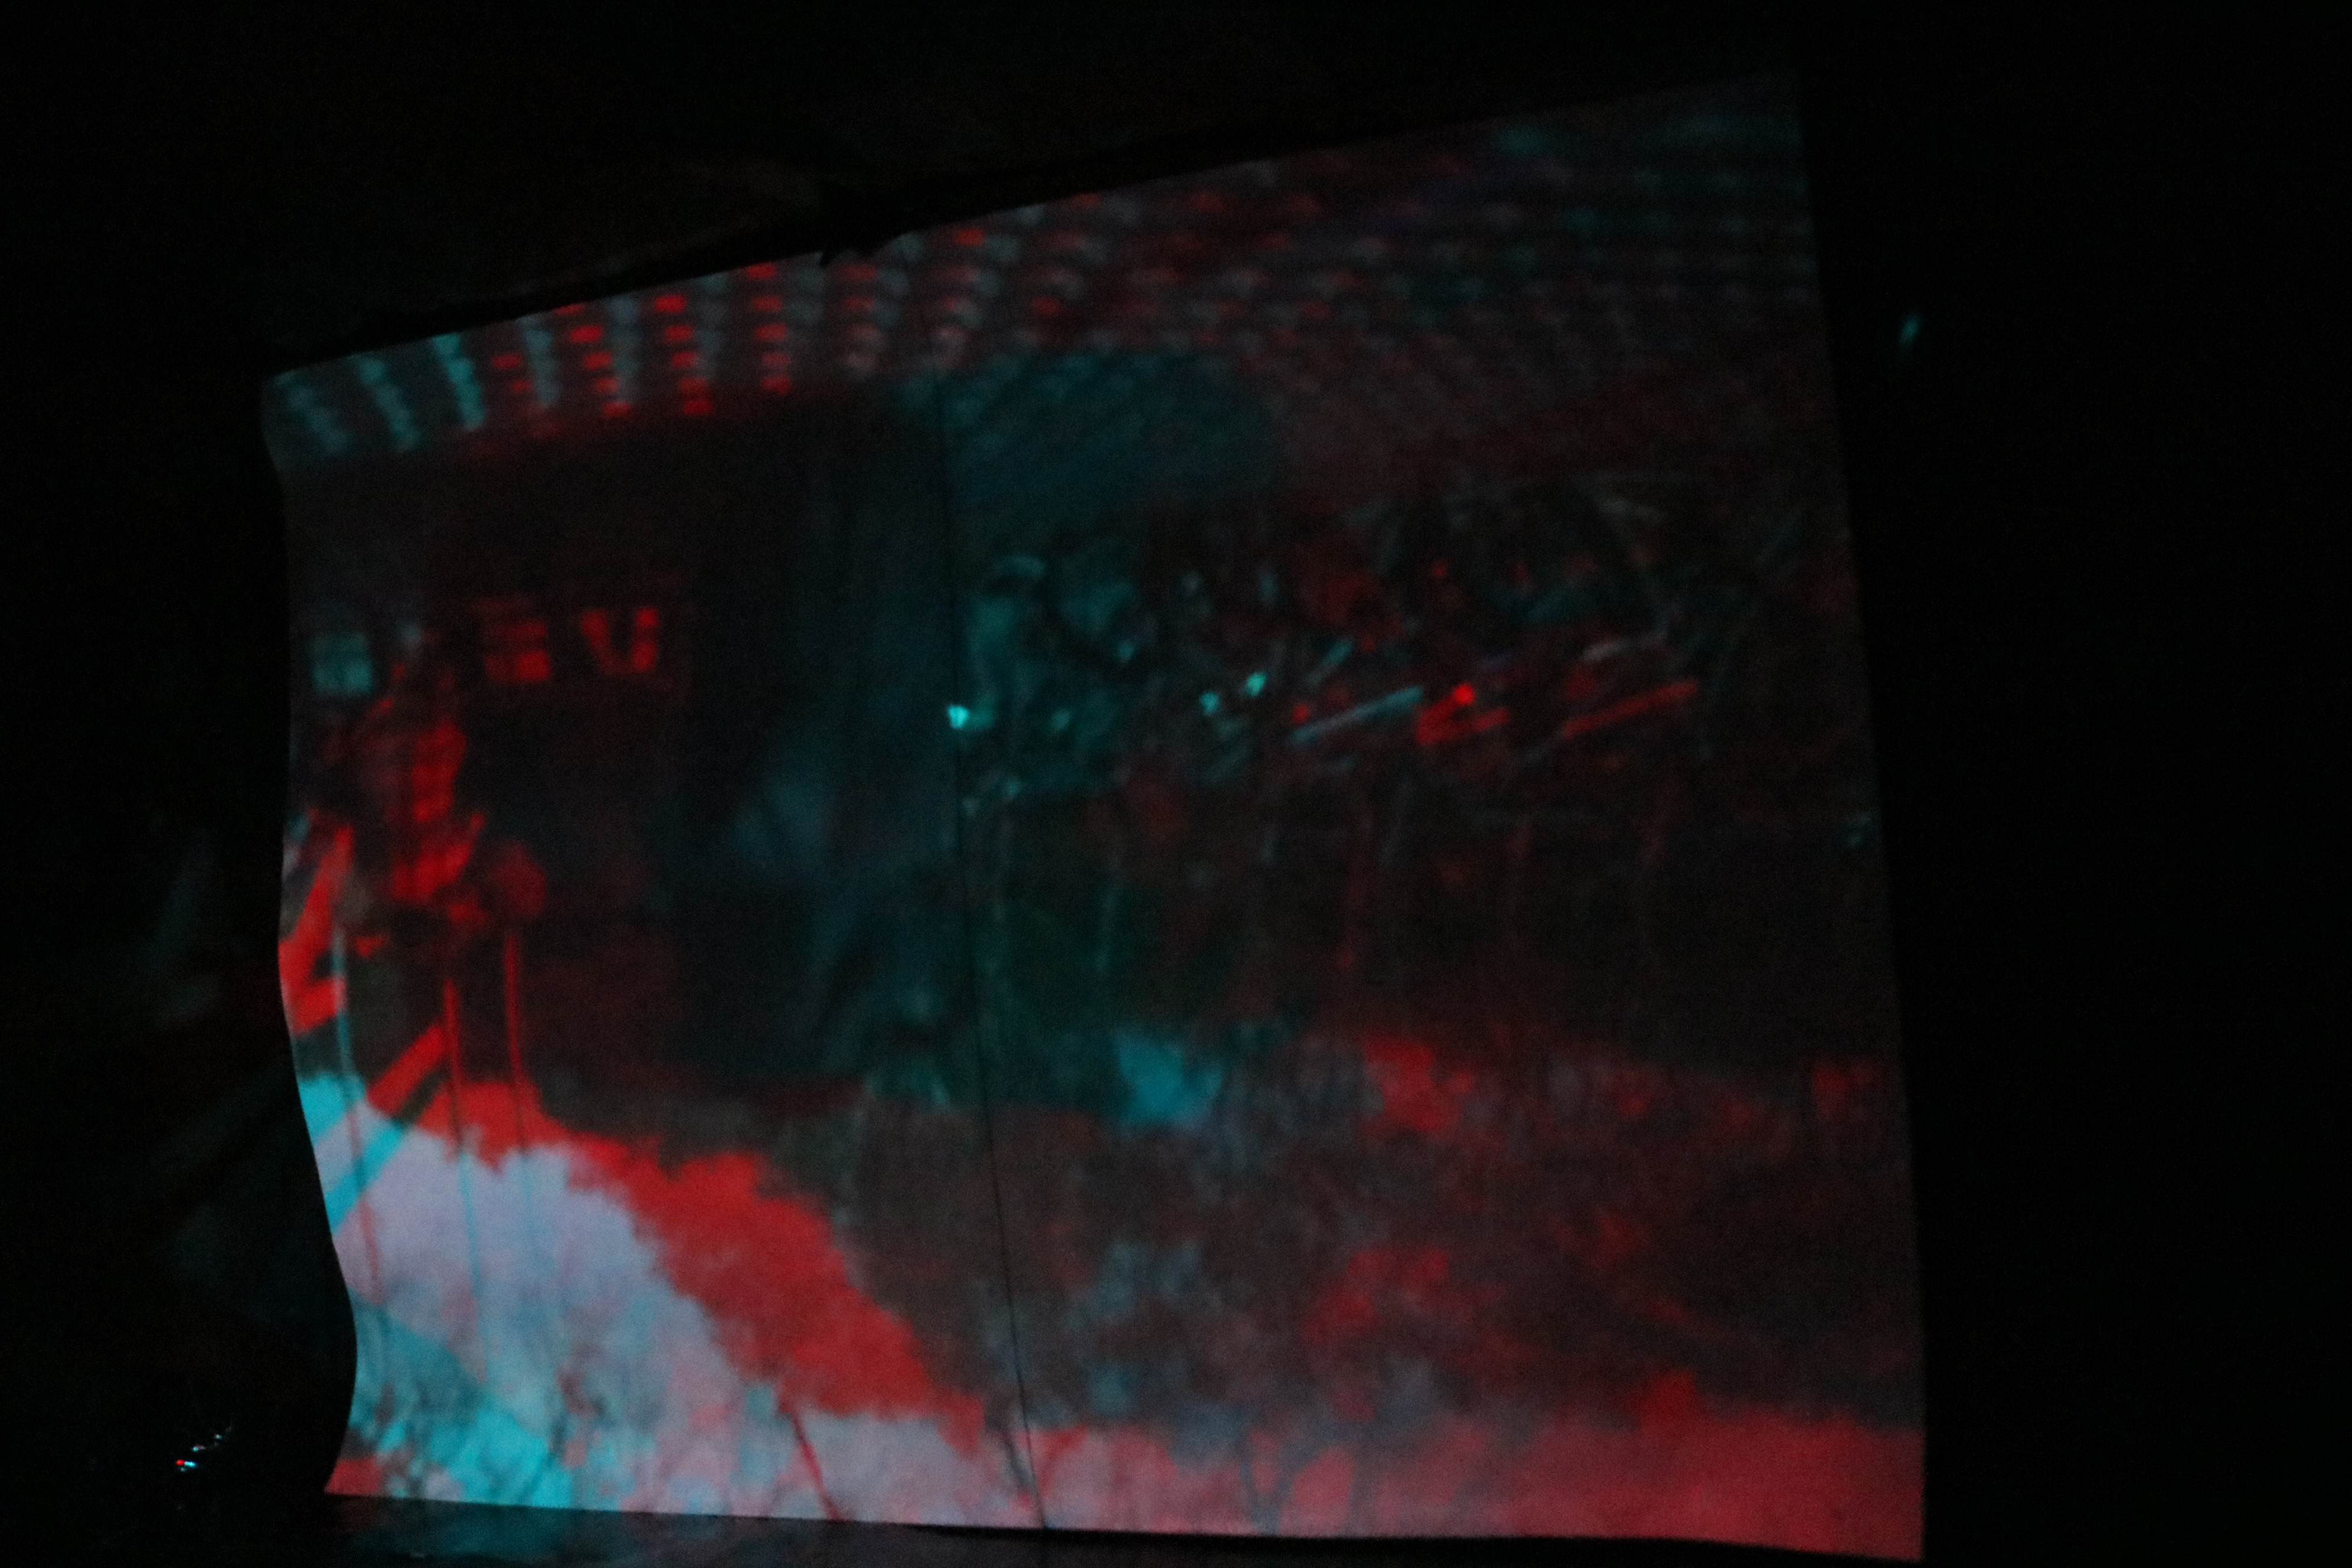
\includegraphics[width=.7\linewidth, height=1in]{IMG_1518.JPG}
		\caption{Scene 2}
	\end{minipage}
	\begin{minipage}[b]{.5\linewidth}
		\centering
		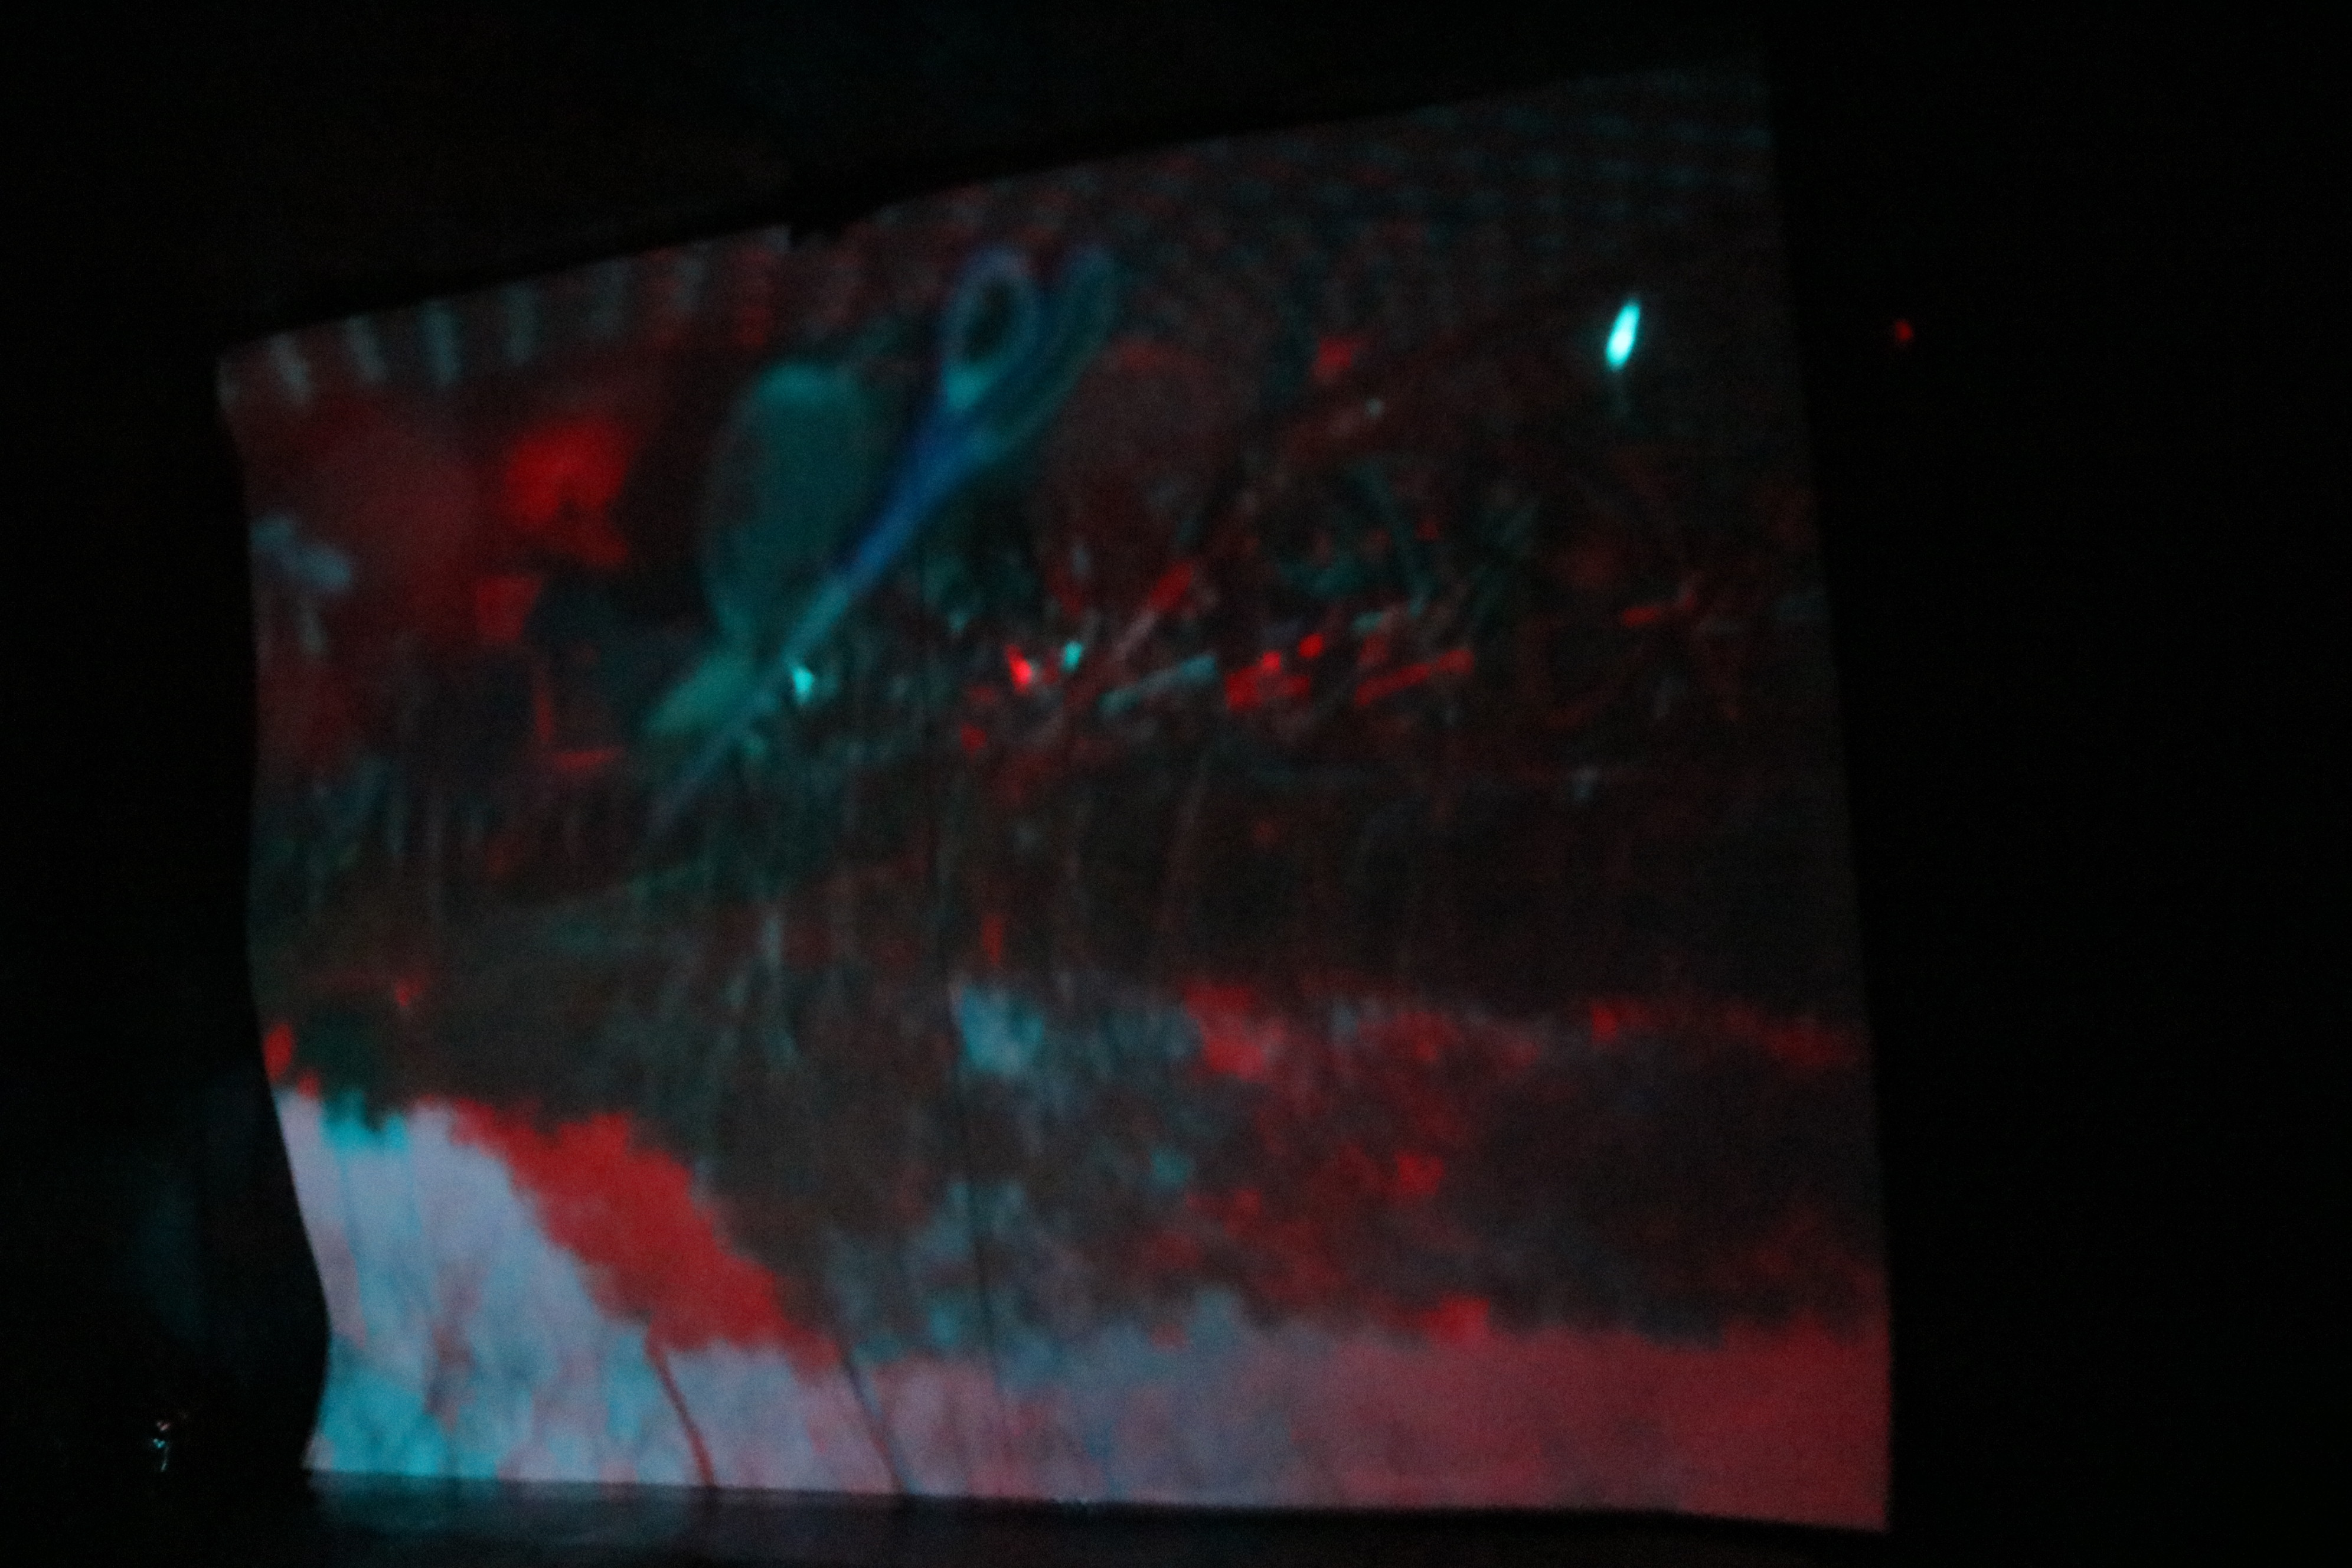
\includegraphics[width=.7\linewidth, height=1in]{IMG_1523.JPG}
		\caption{Scene 3}
	\end{minipage}
	\begin{minipage}[b]{.5\linewidth}
		\centering
		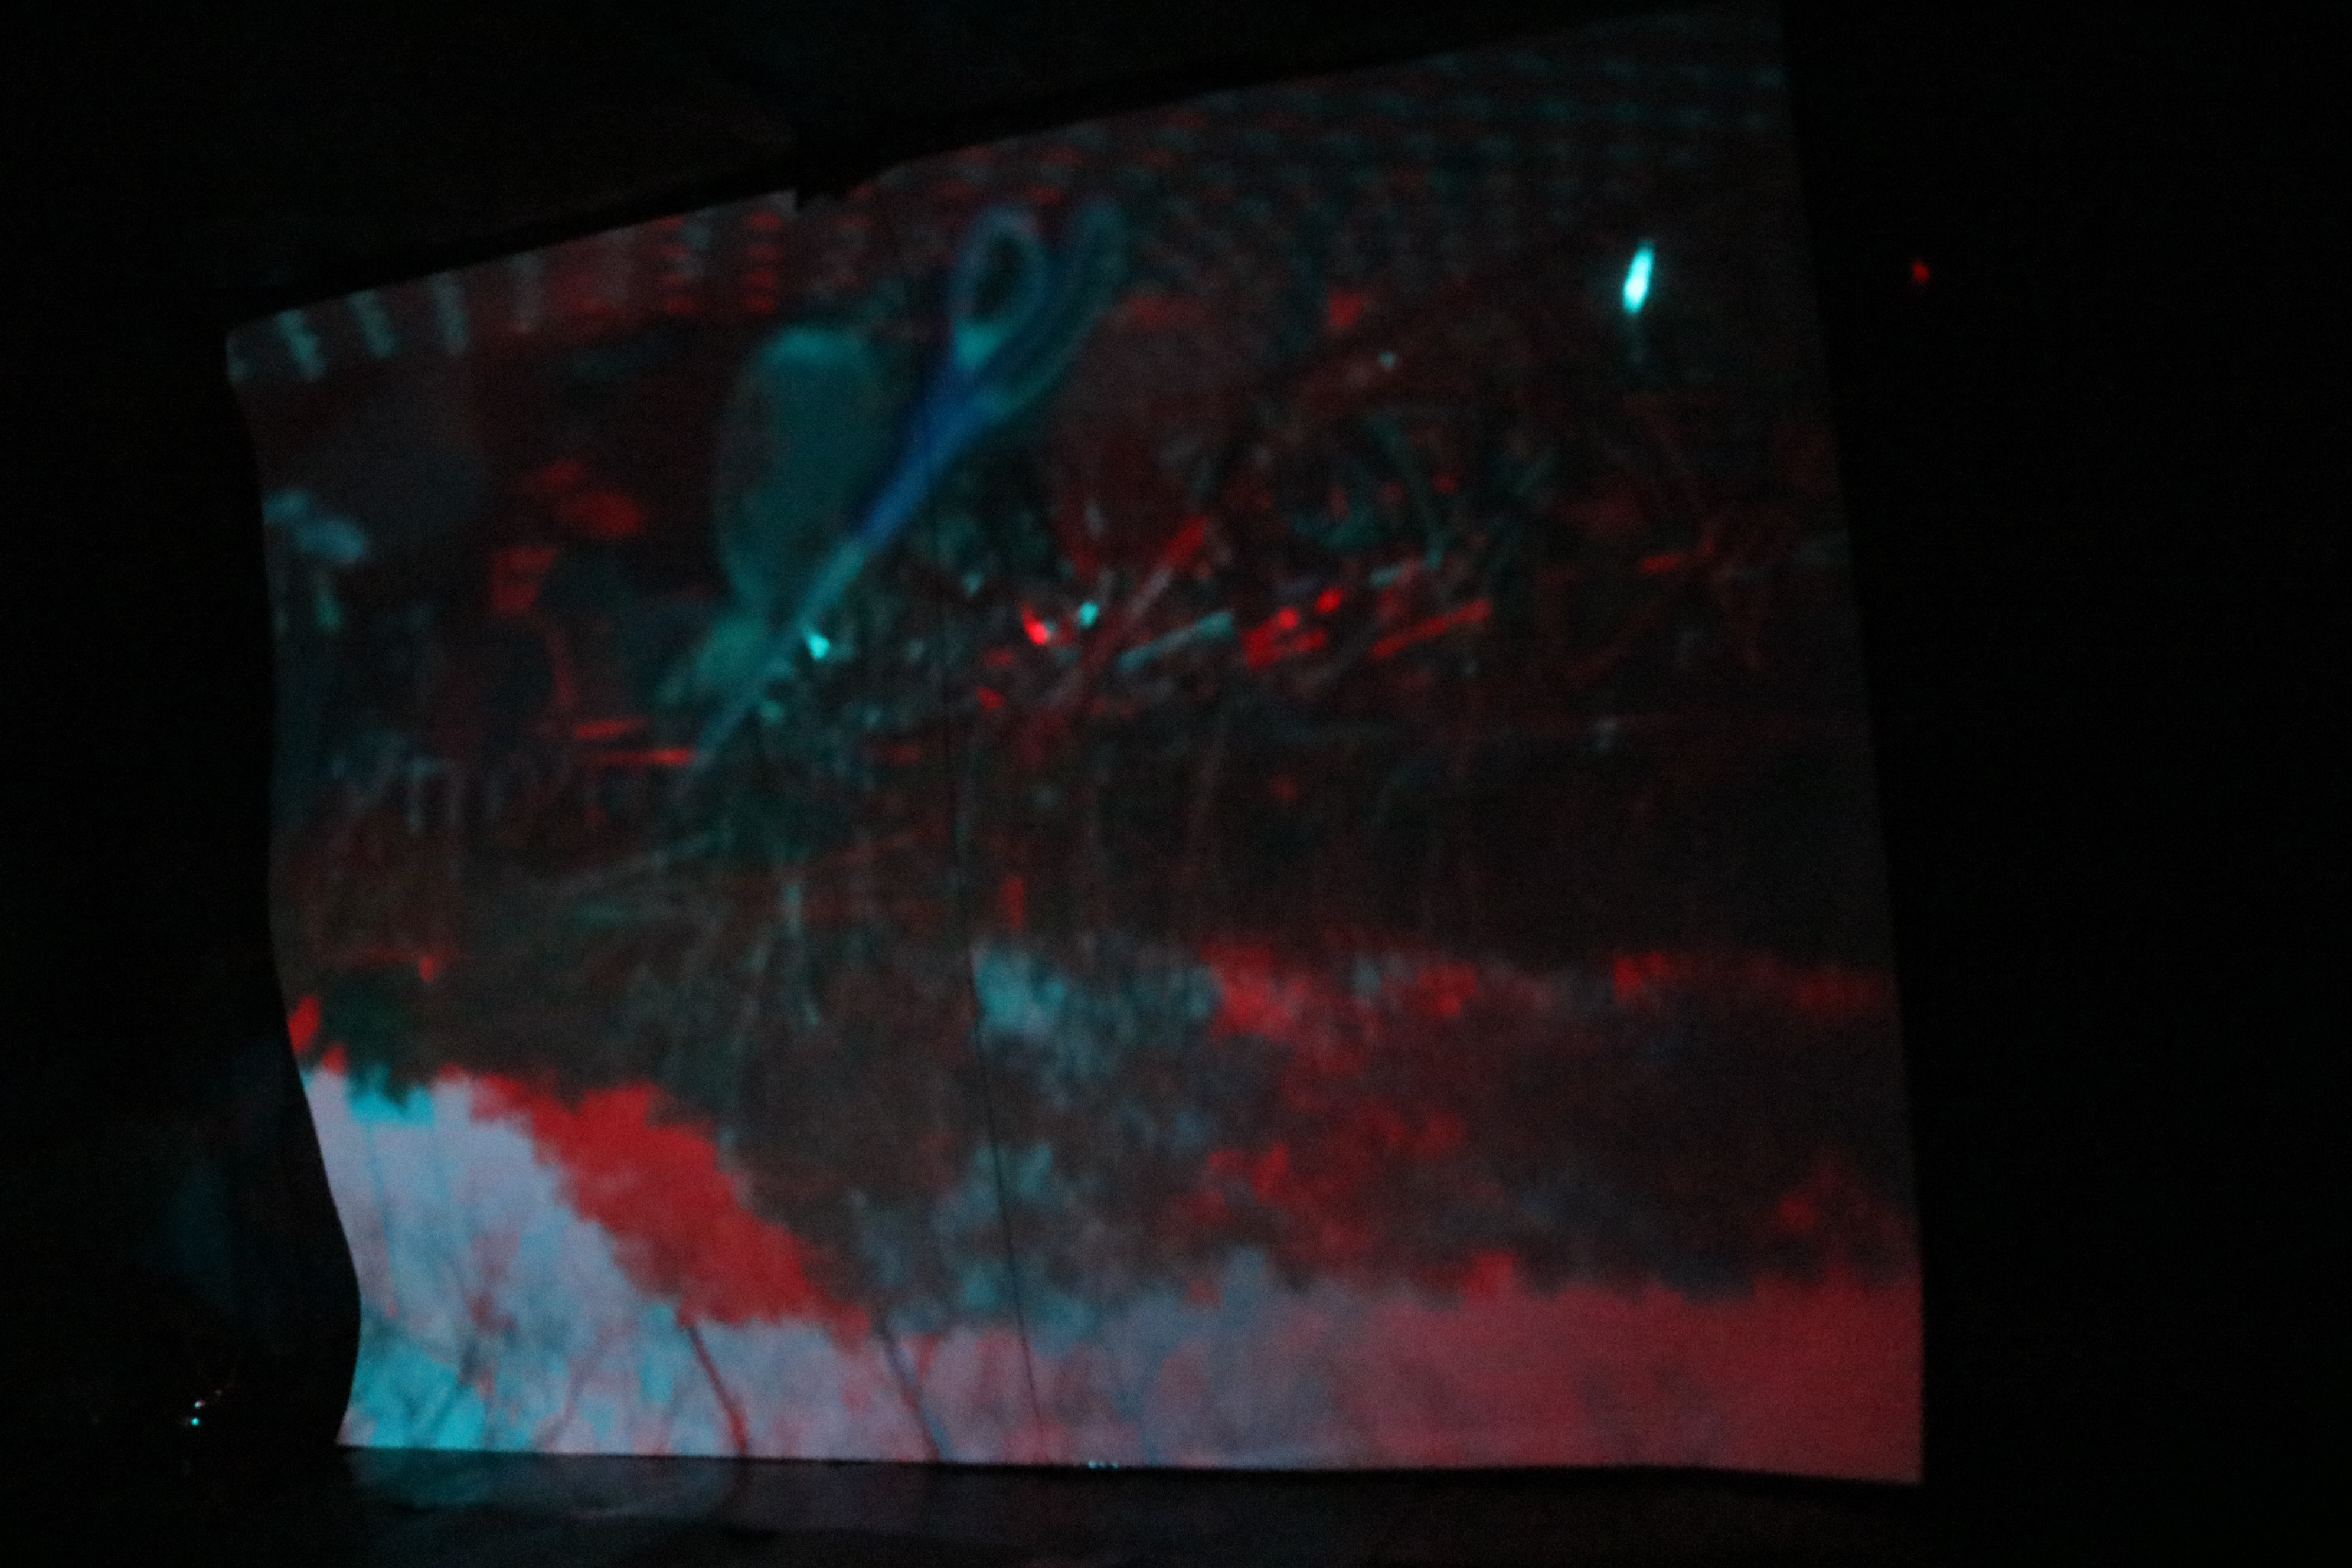
\includegraphics[width=.7\linewidth, height=1in]{IMG_1525.JPG}
		\caption{Scene 4}
	\end{minipage}
	\begin{minipage}[b]{.5\linewidth}
		\centering
		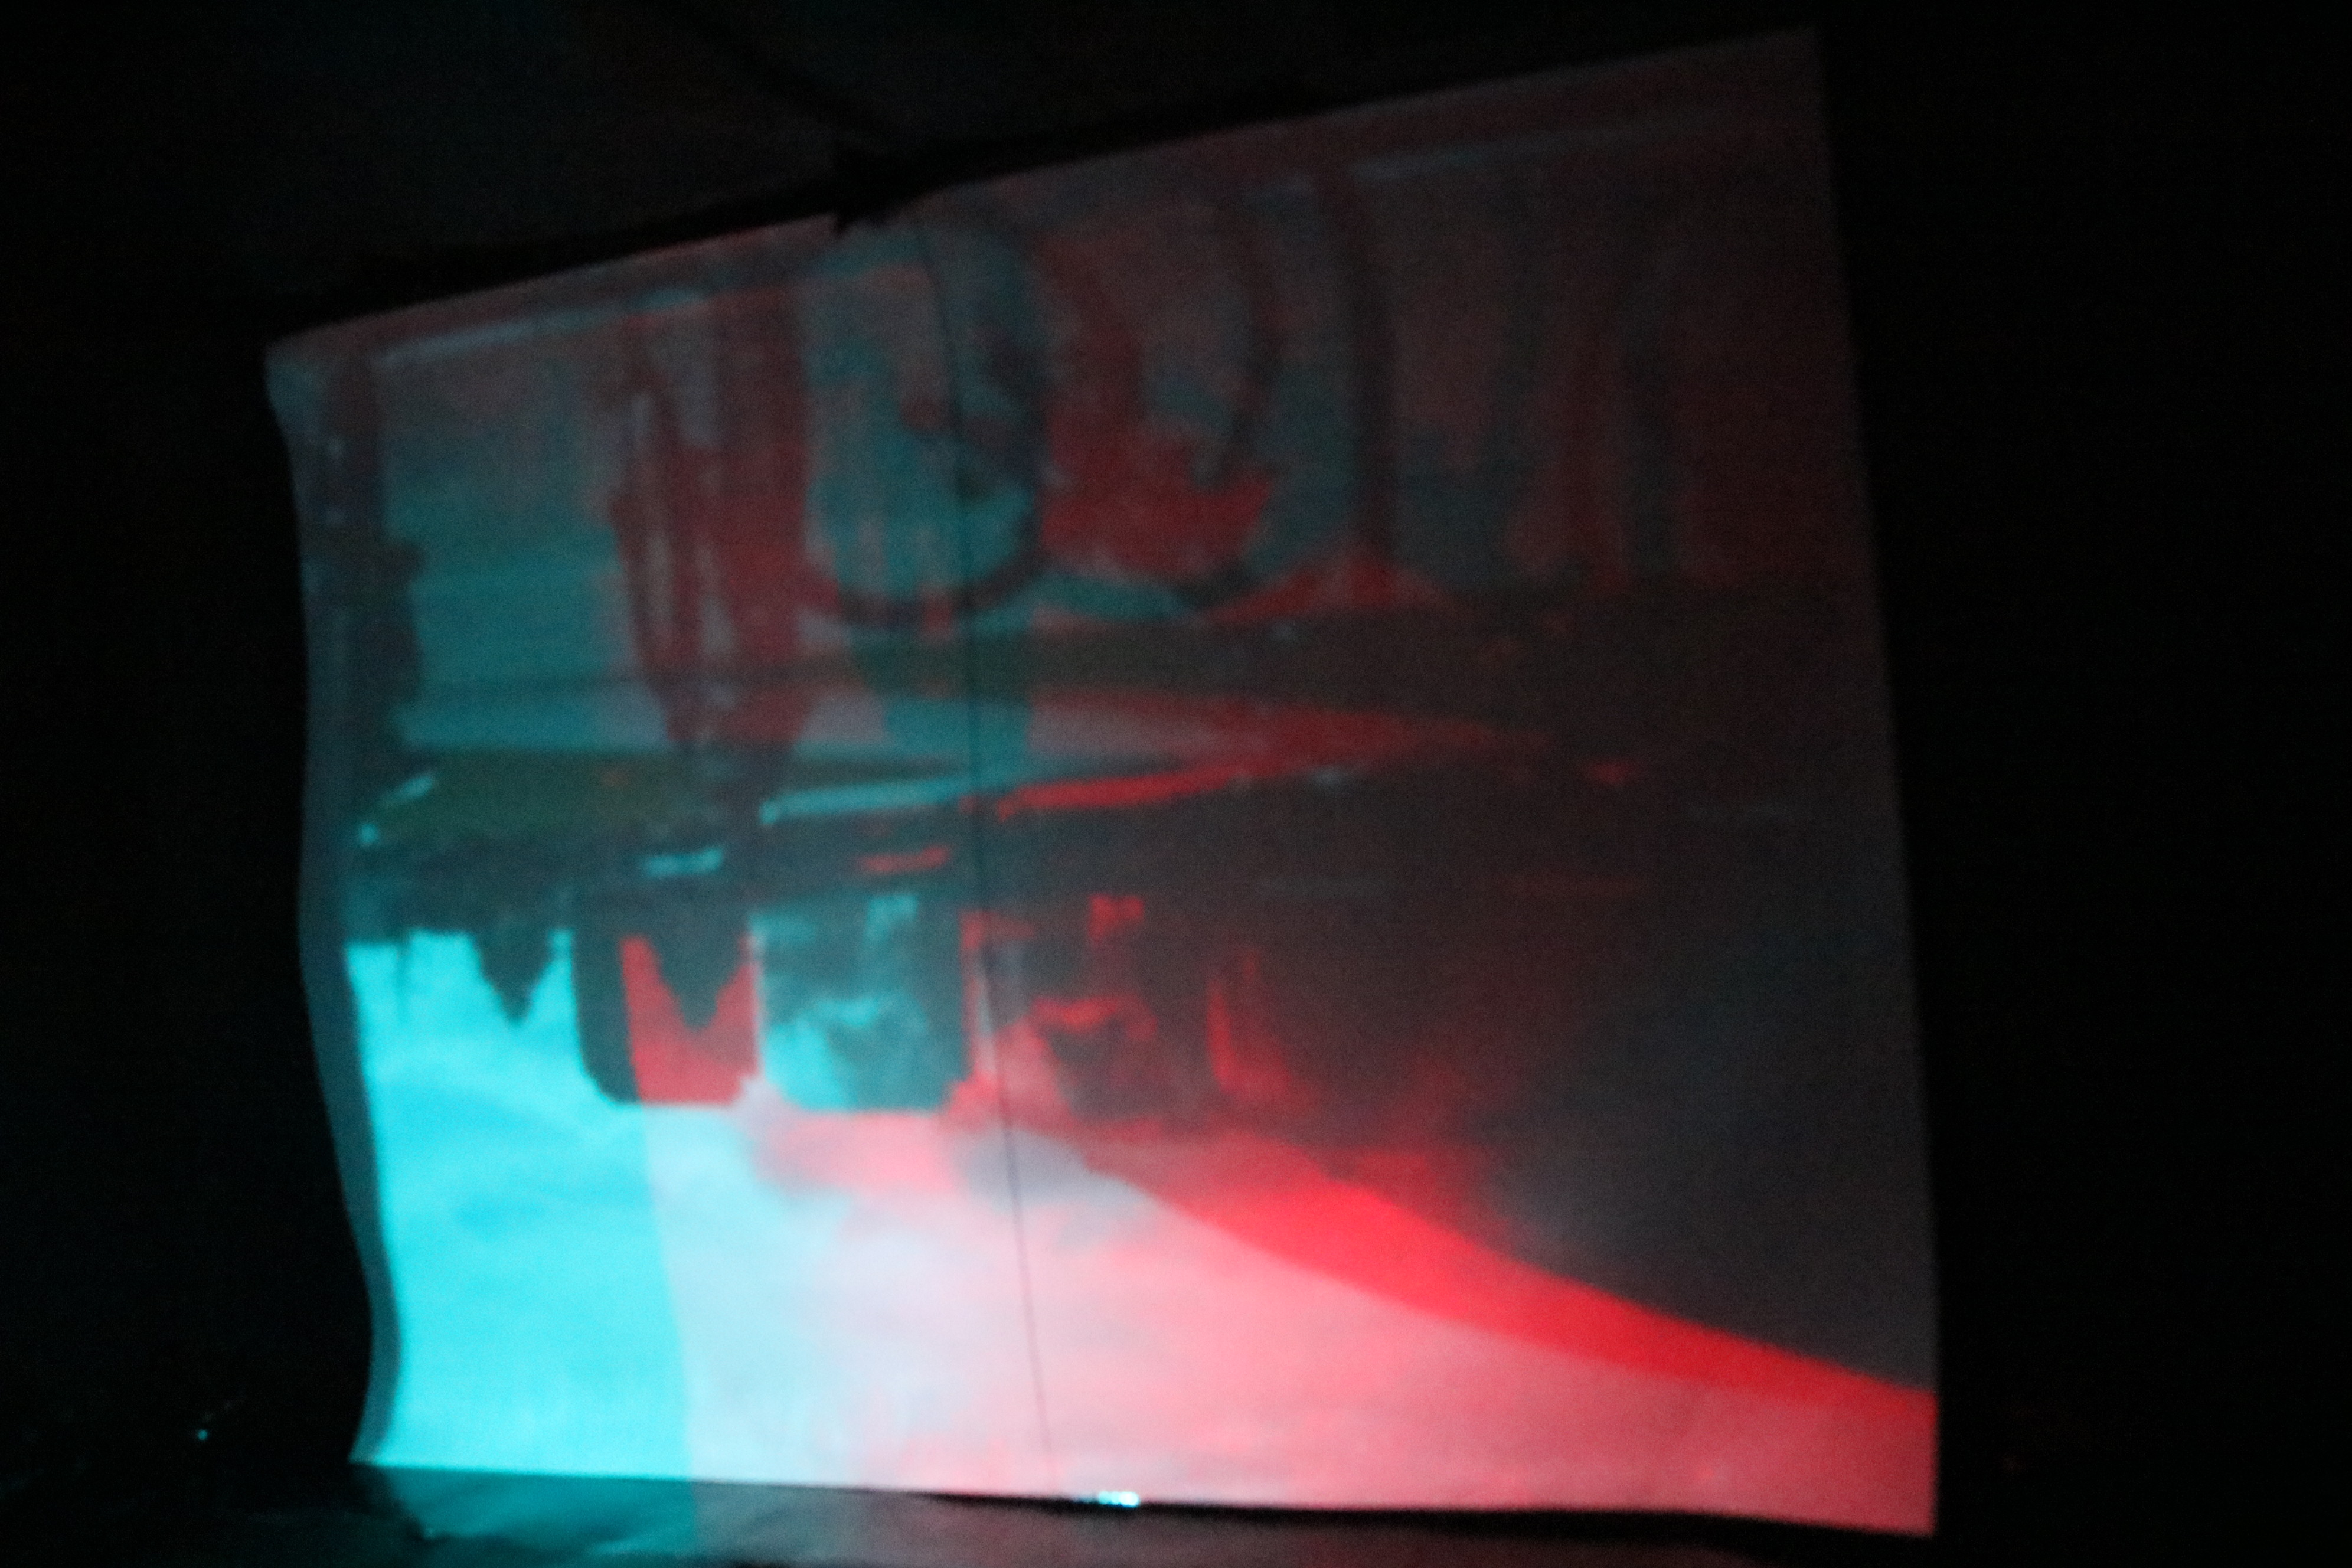
\includegraphics[width=.7\linewidth, height=1in]{IMG_1486.JPG}
		\caption{Scene 5}
	\end{minipage}
	\end{figure}
	

\newline \emph{\textbf{3. Calibration and Image Correction}}
\begin{document}
\begin{figure}[H]
	\centering
	\begin{minipage}[b]{.5\linewidth}
		\centering
		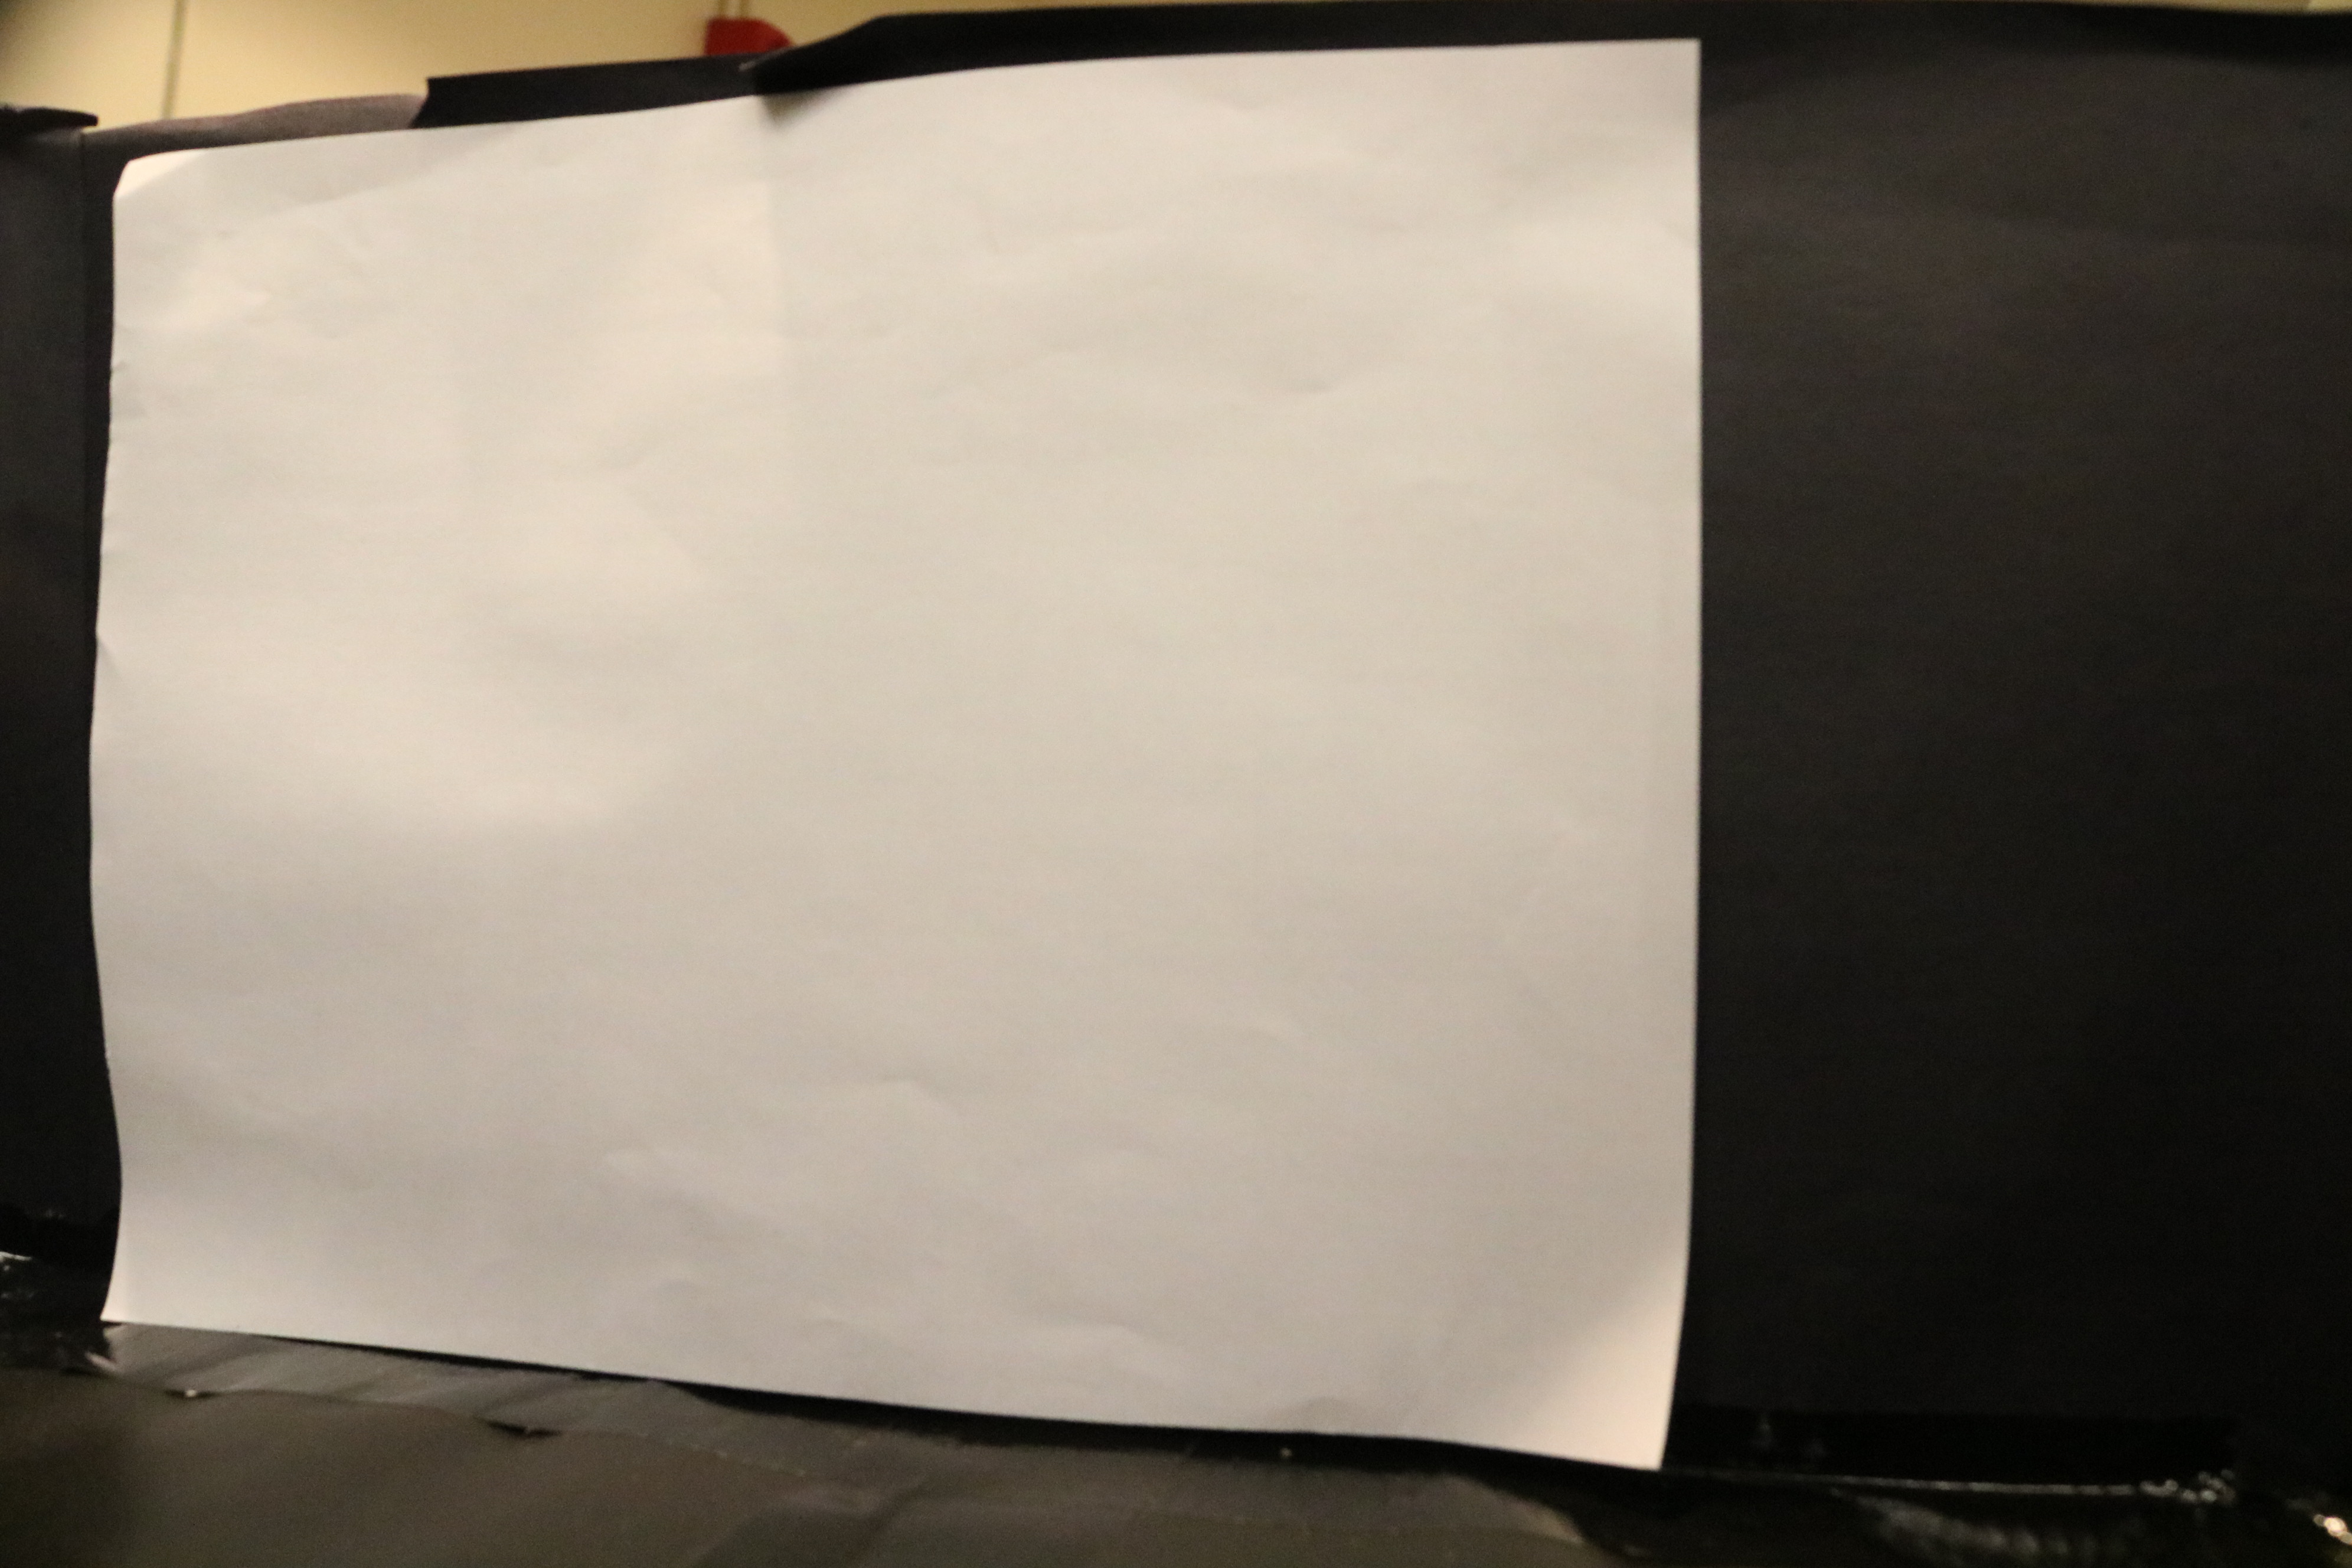
\includegraphics[width=.7\linewidth, height=1in]{ref.jpg}
		\caption{Distorted Image}
	\end{minipage}
	\begin{minipage}[b]{.5\linewidth}
		\centering
		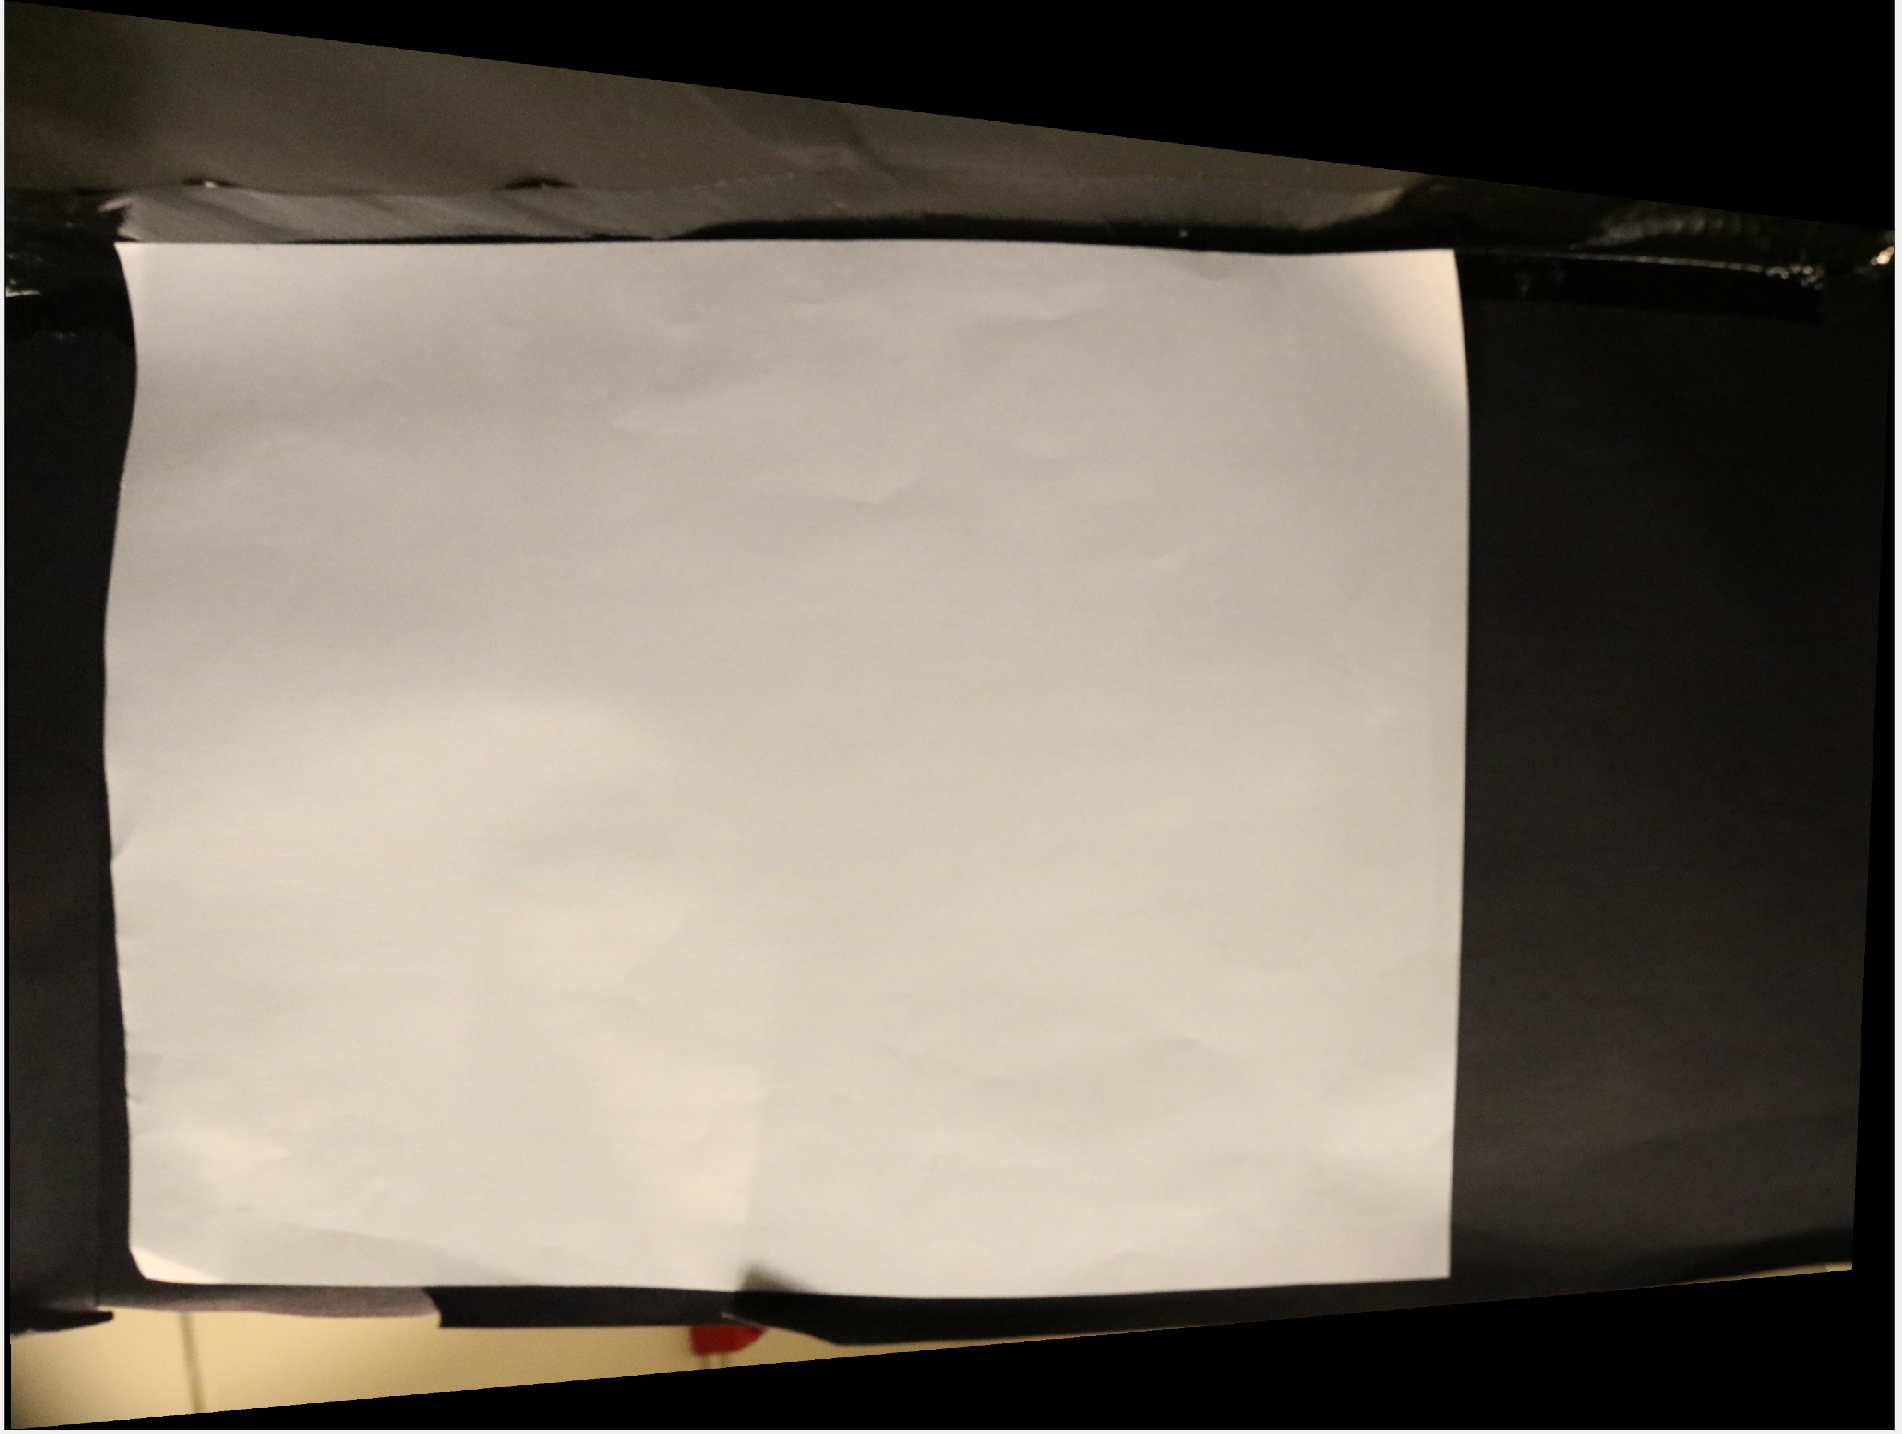
\includegraphics[width=.7\linewidth, height=1in]{corrected.jpg}
		\caption{Corrected Image}
	\end{minipage}
\end{figure}

\newline \emph{\textbf{4. Anaglyph Camera Obscura: A device to Measure Distances to Objects }}
\newline \emph{An analytical expression that relates the distance between the two spots in
the picture with the distance of the light with respect to the camera and the parameters of
the camera (distance to the back wall, separation between the two holes, etc.)}
\begin{document}
 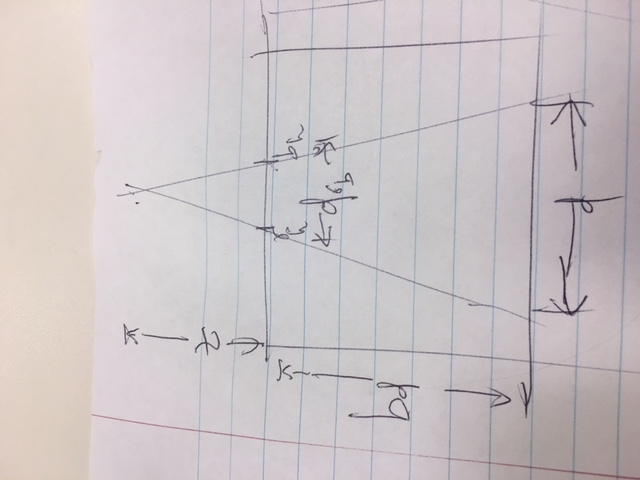
\includegraphics[width=4cm,height=4cm]{proof.jpg}
 \newline Picture for proving relationship between $z$ and $d$
\end{figure}
\newline $b_d=$ box distance 
\newline $z=$ distane of light from pinhole
\newline $d_{RB}=$ distance between red and blue holes
\newline $d=$ distance between two lights cast on the white paper
\newline Using similarity of triangles , 
\newline $\frac{z}{d_{RB}}=\frac{z+b_{d}}{d}$
\newline $zd=zd_{RB}+b_{d}d_{RB}$
\newline $zd-zd_{RB}=b_{d}d_{RB}$
\newline $z(d-d_{RB})=b_{d}d_{RB}$
\newline $z=\frac{b_{d}d_{RB}}{(d-d_{RB})}$
\newline Using $1$ inch = $247.2727$ image distance units, and the above formula , we can plots
values for $z$ and compare to those taken by camera with pre-known $ds$ or vice versa
	\begin{document}
	\begin{figure}[H]
	\centering
	\begin{minipage}[b]{.5\linewidth}
		\centering
		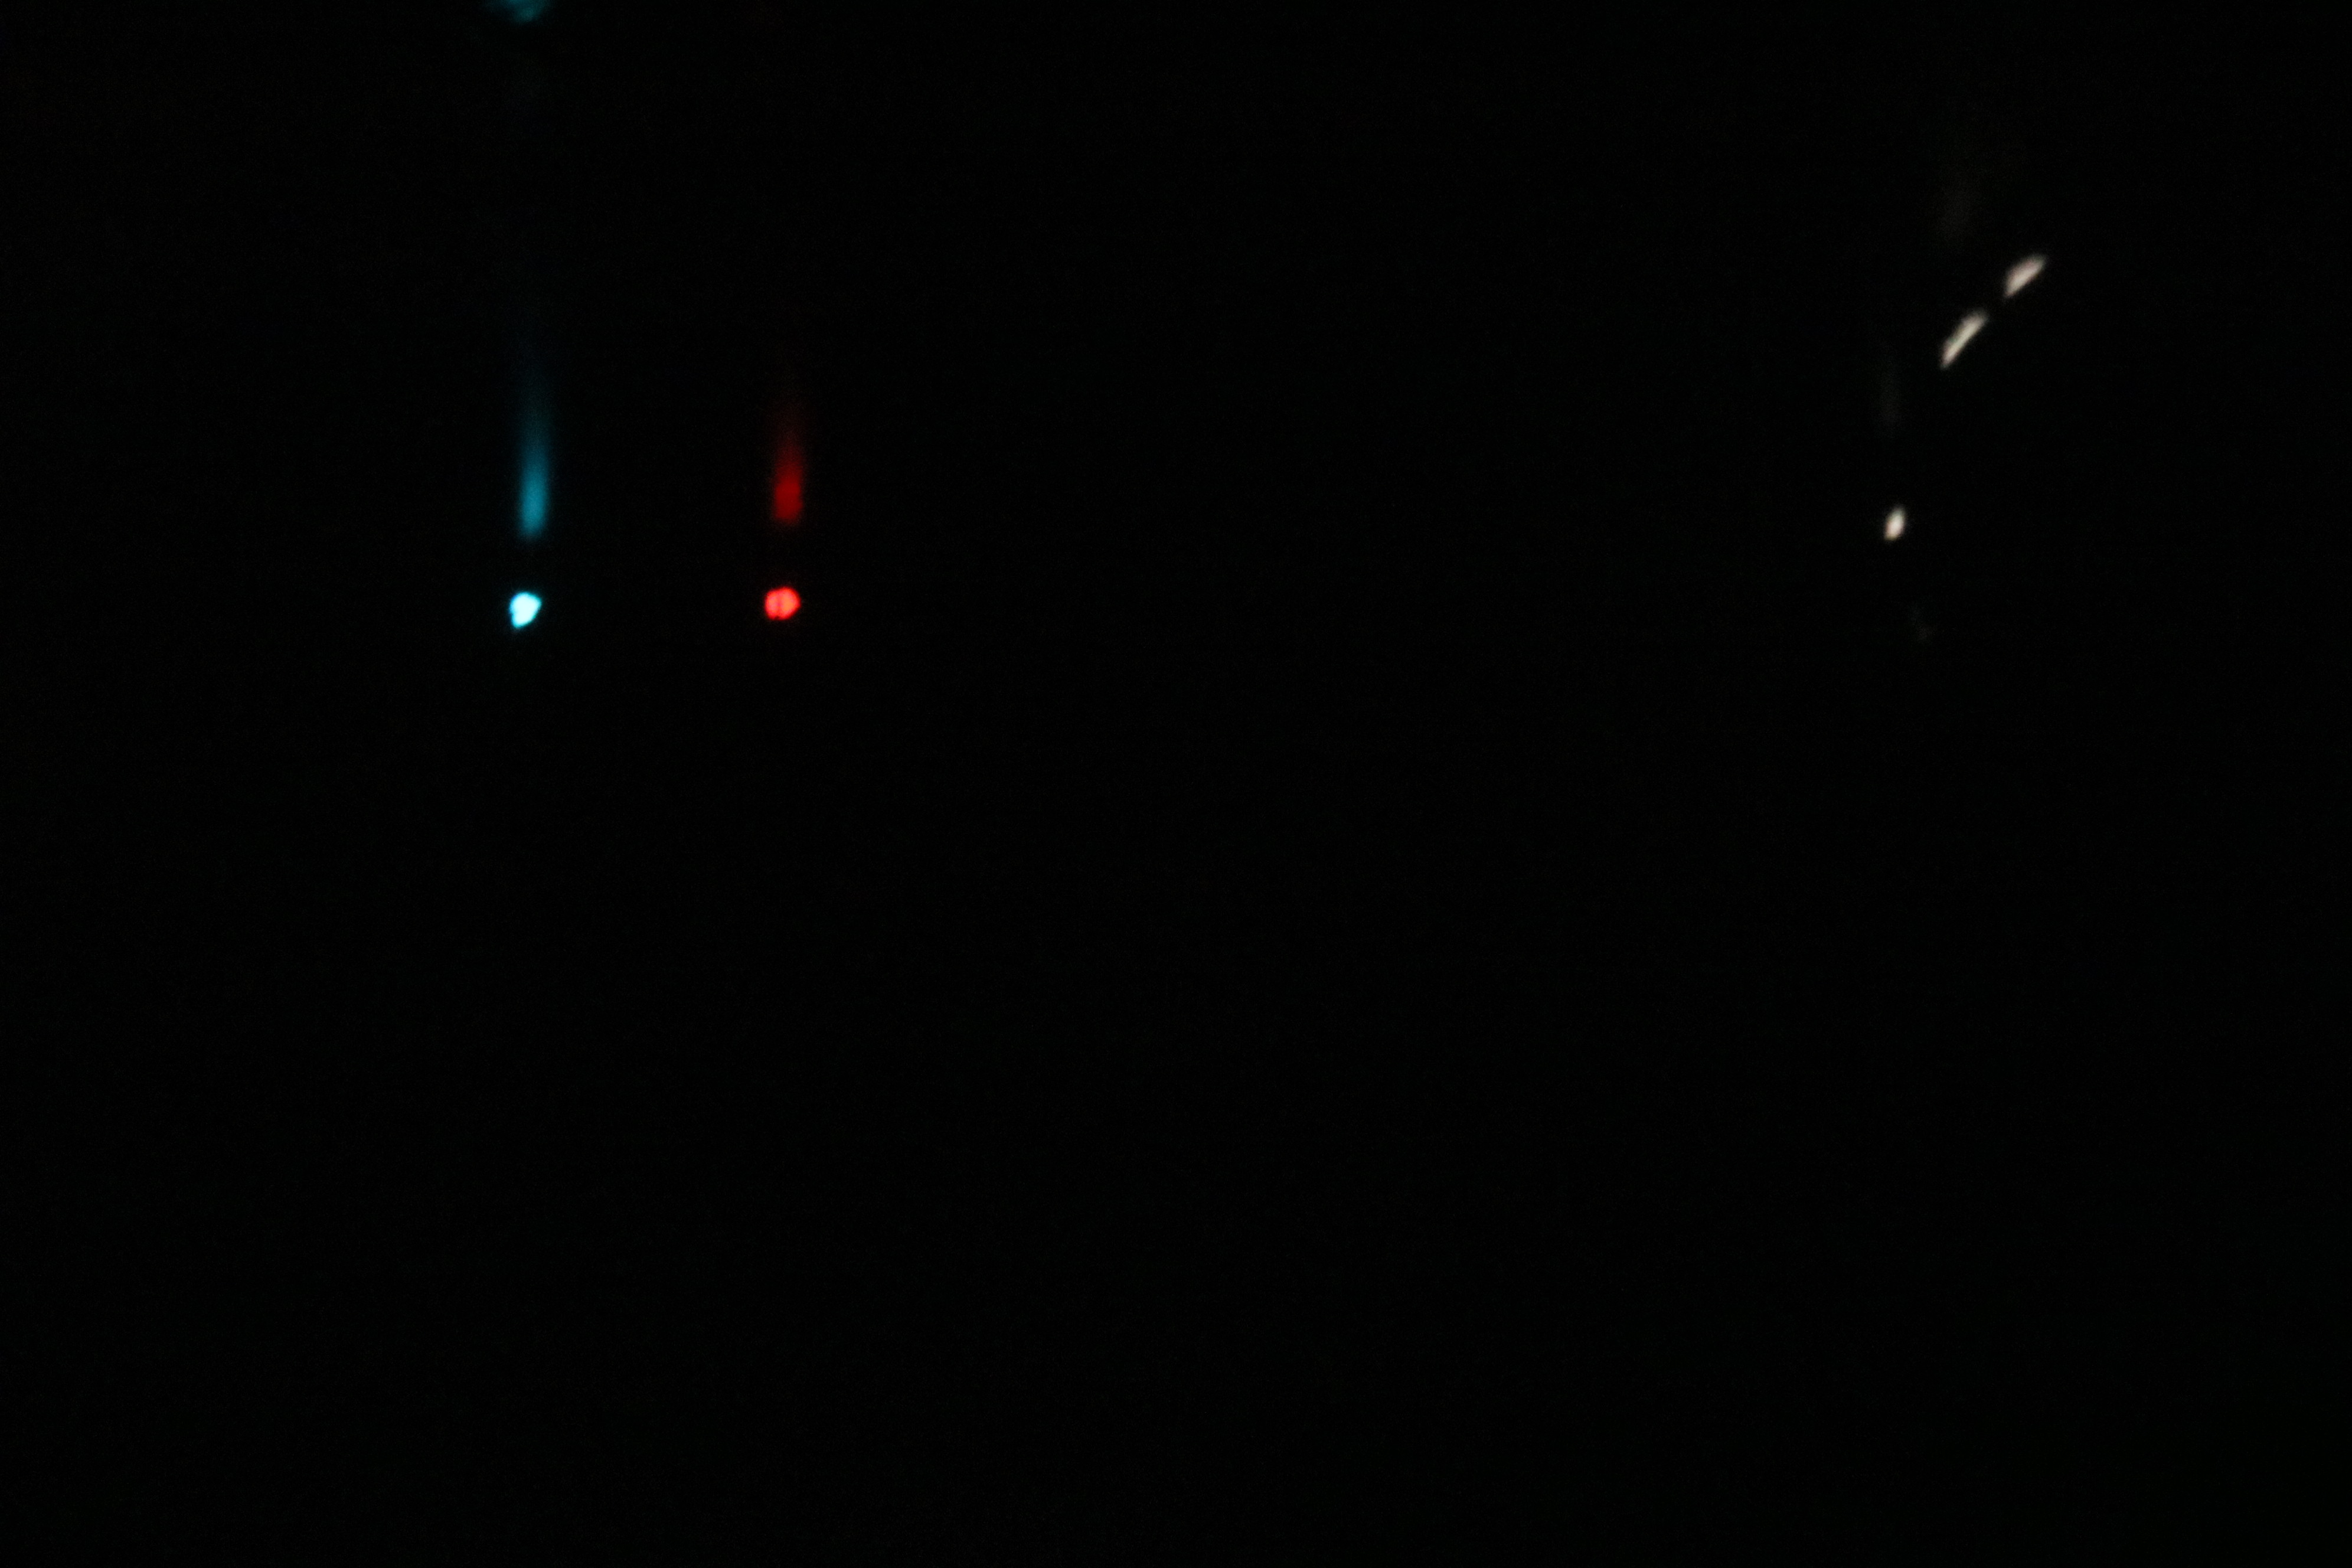
\includegraphics[width=.7\linewidth, height=1in]{z_17in_take_3.JPG}
		\caption{z=17 inches}
	\end{minipage}
	\begin{minipage}[b]{.5\linewidth}
		\centering
		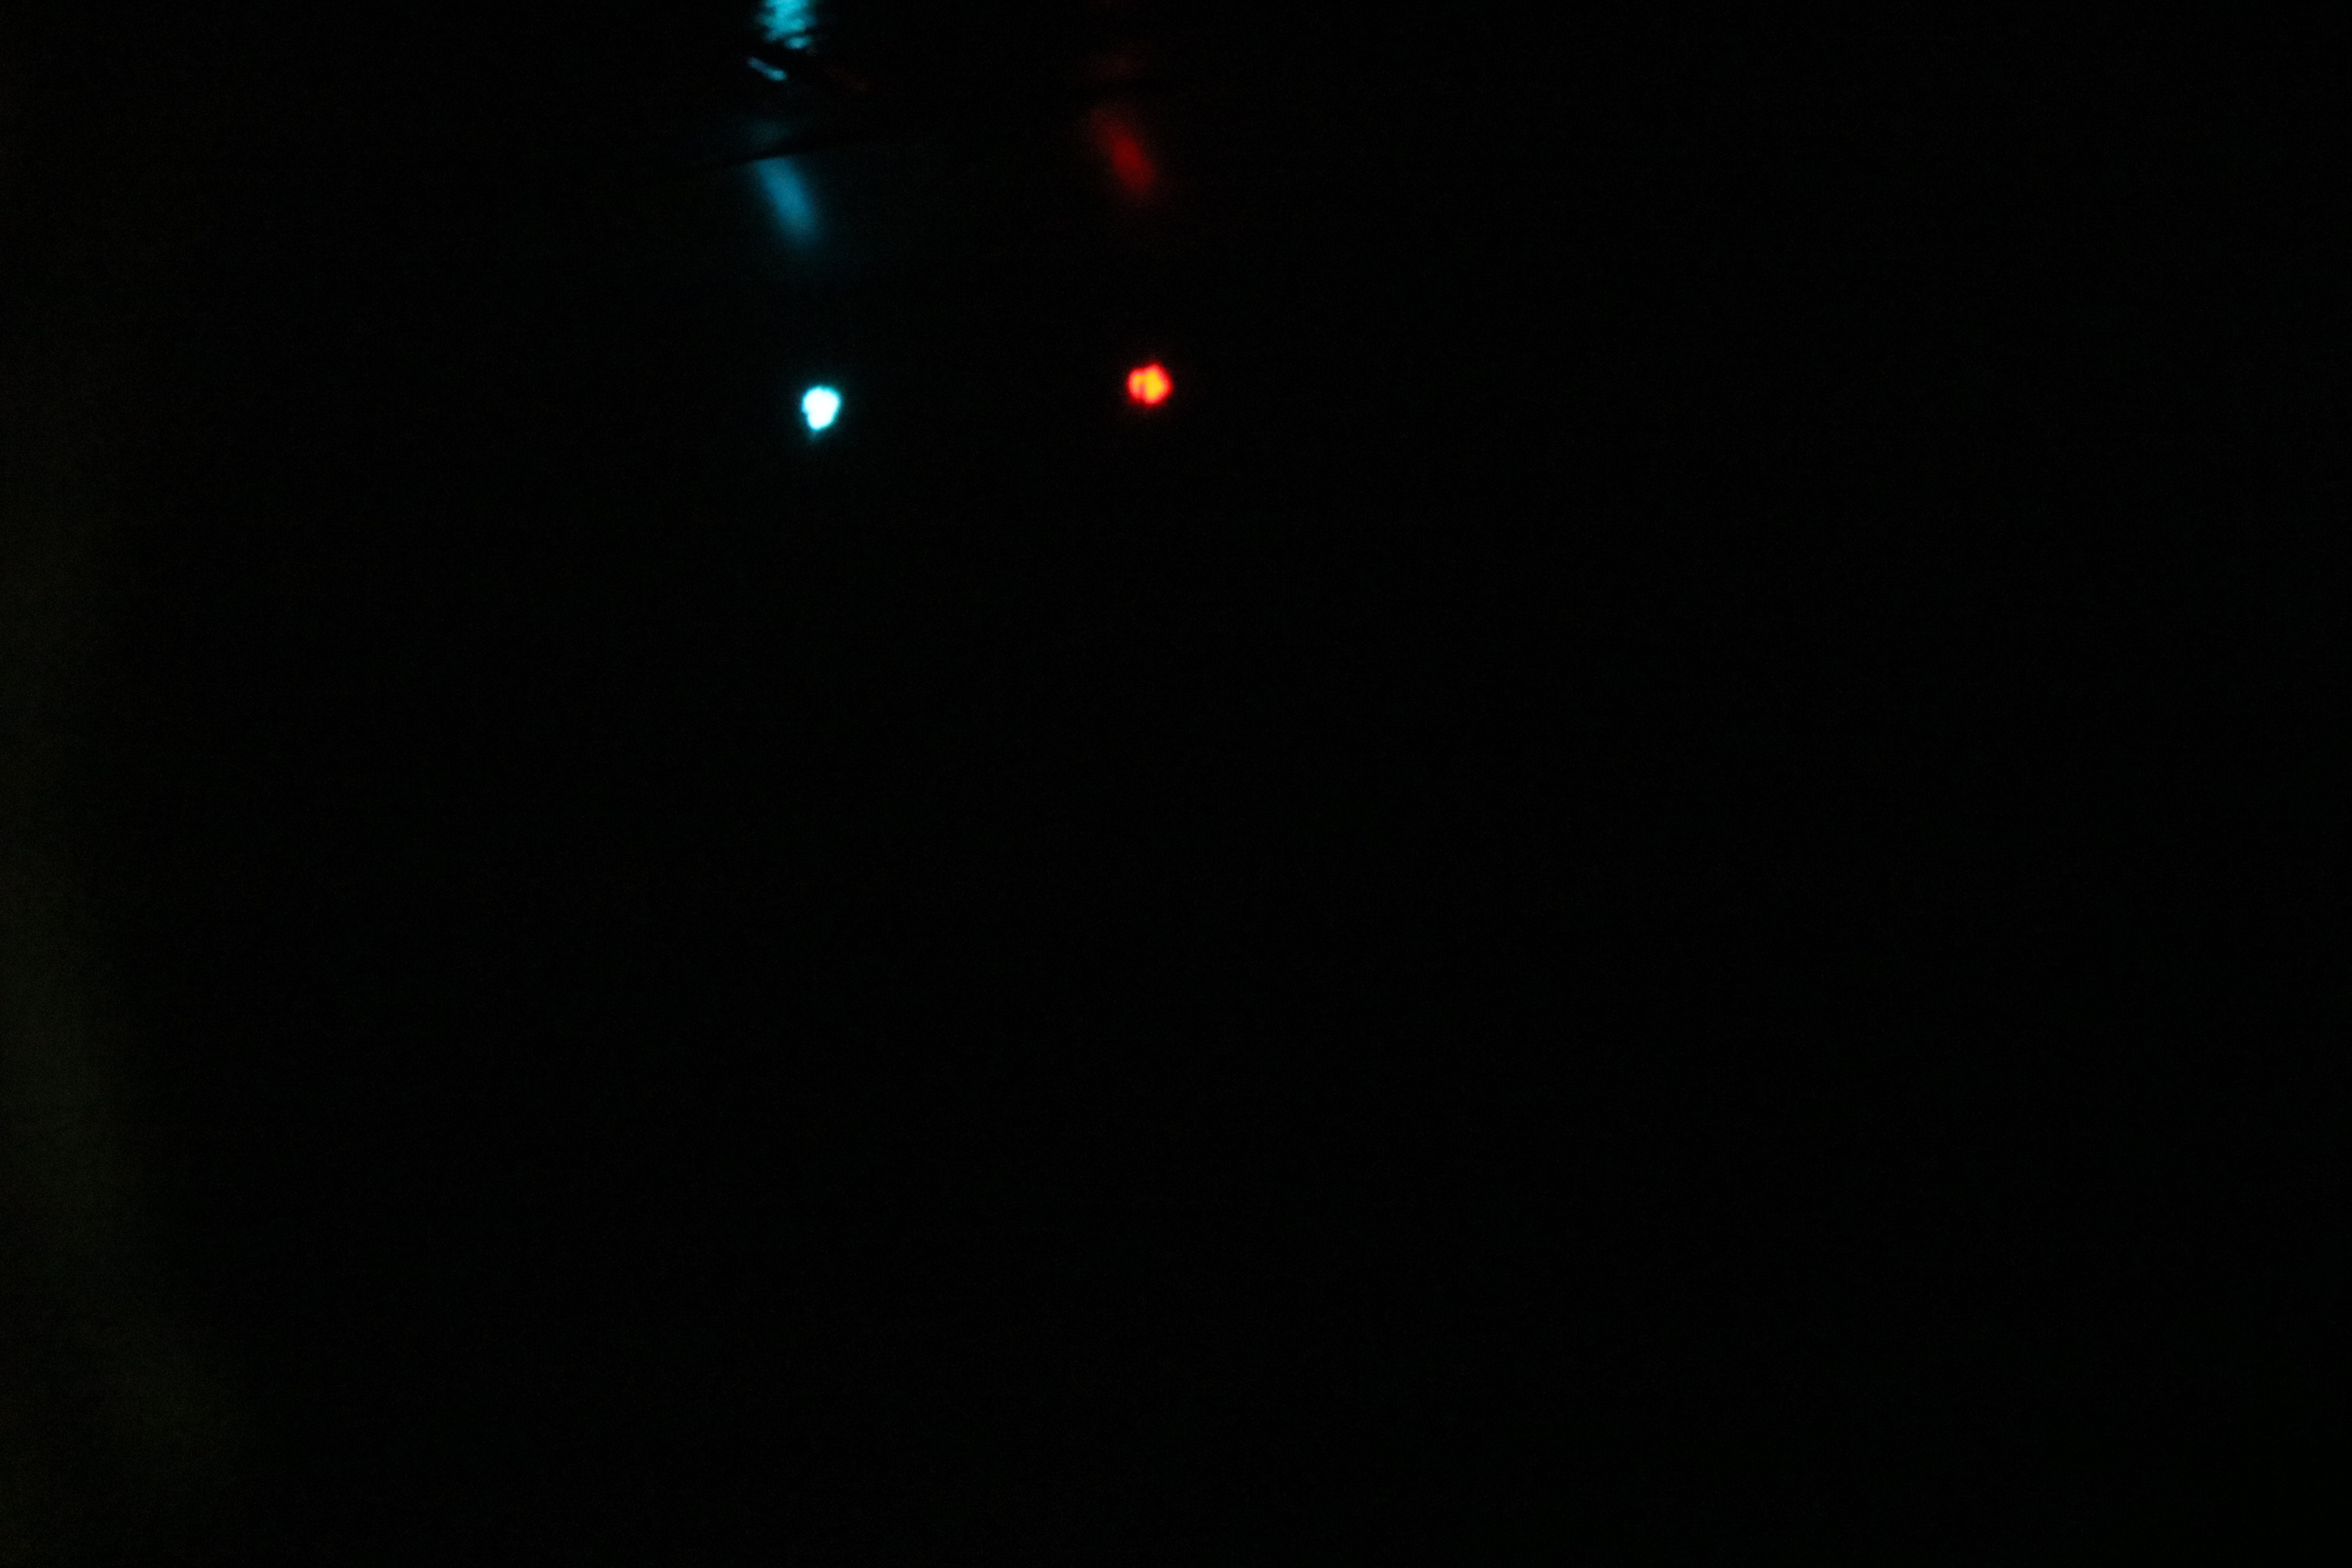
\includegraphics[width=.7\linewidth, height=1in]{z_34in.JPG}
		\caption{z=34 inches}
	\end{minipage}
	\begin{minipage}[b]{.5\linewidth}
		\centering
		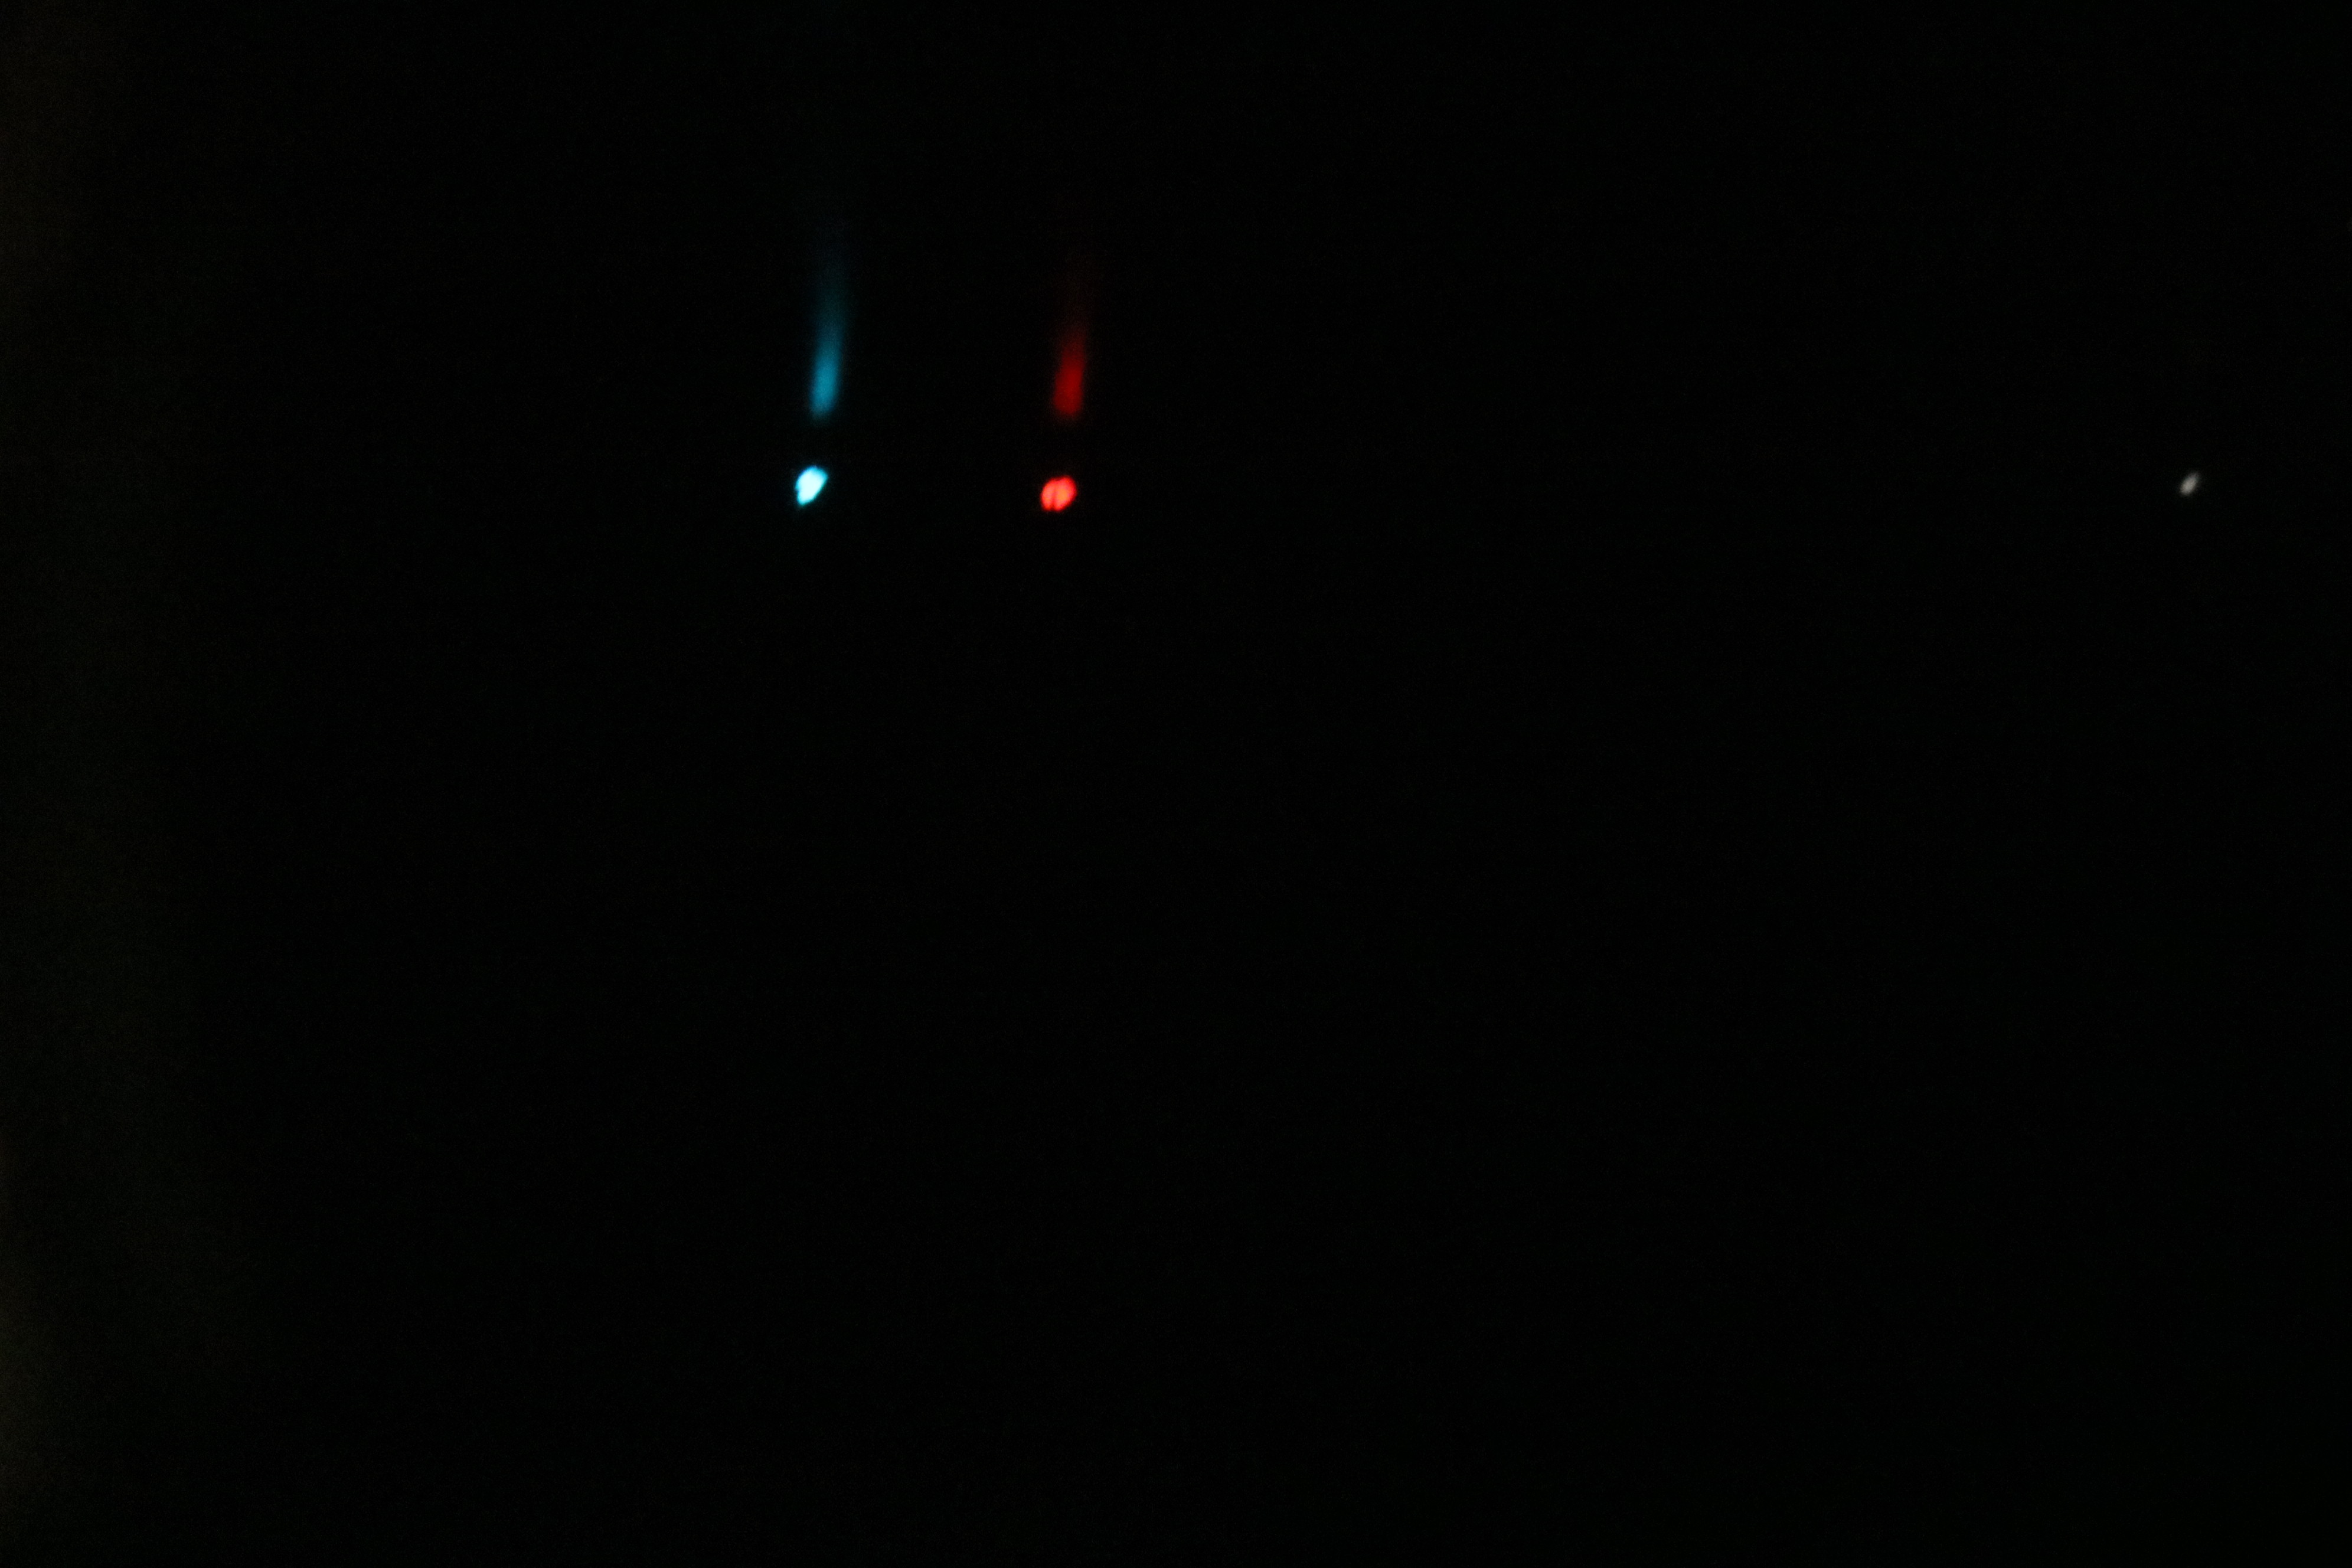
\includegraphics[width=.7\linewidth, height=1in]{z_51in.JPG}
		\caption{z=51 inches}
	\end{minipage}
	\begin{minipage}[b]{.5\linewidth}
		\centering
		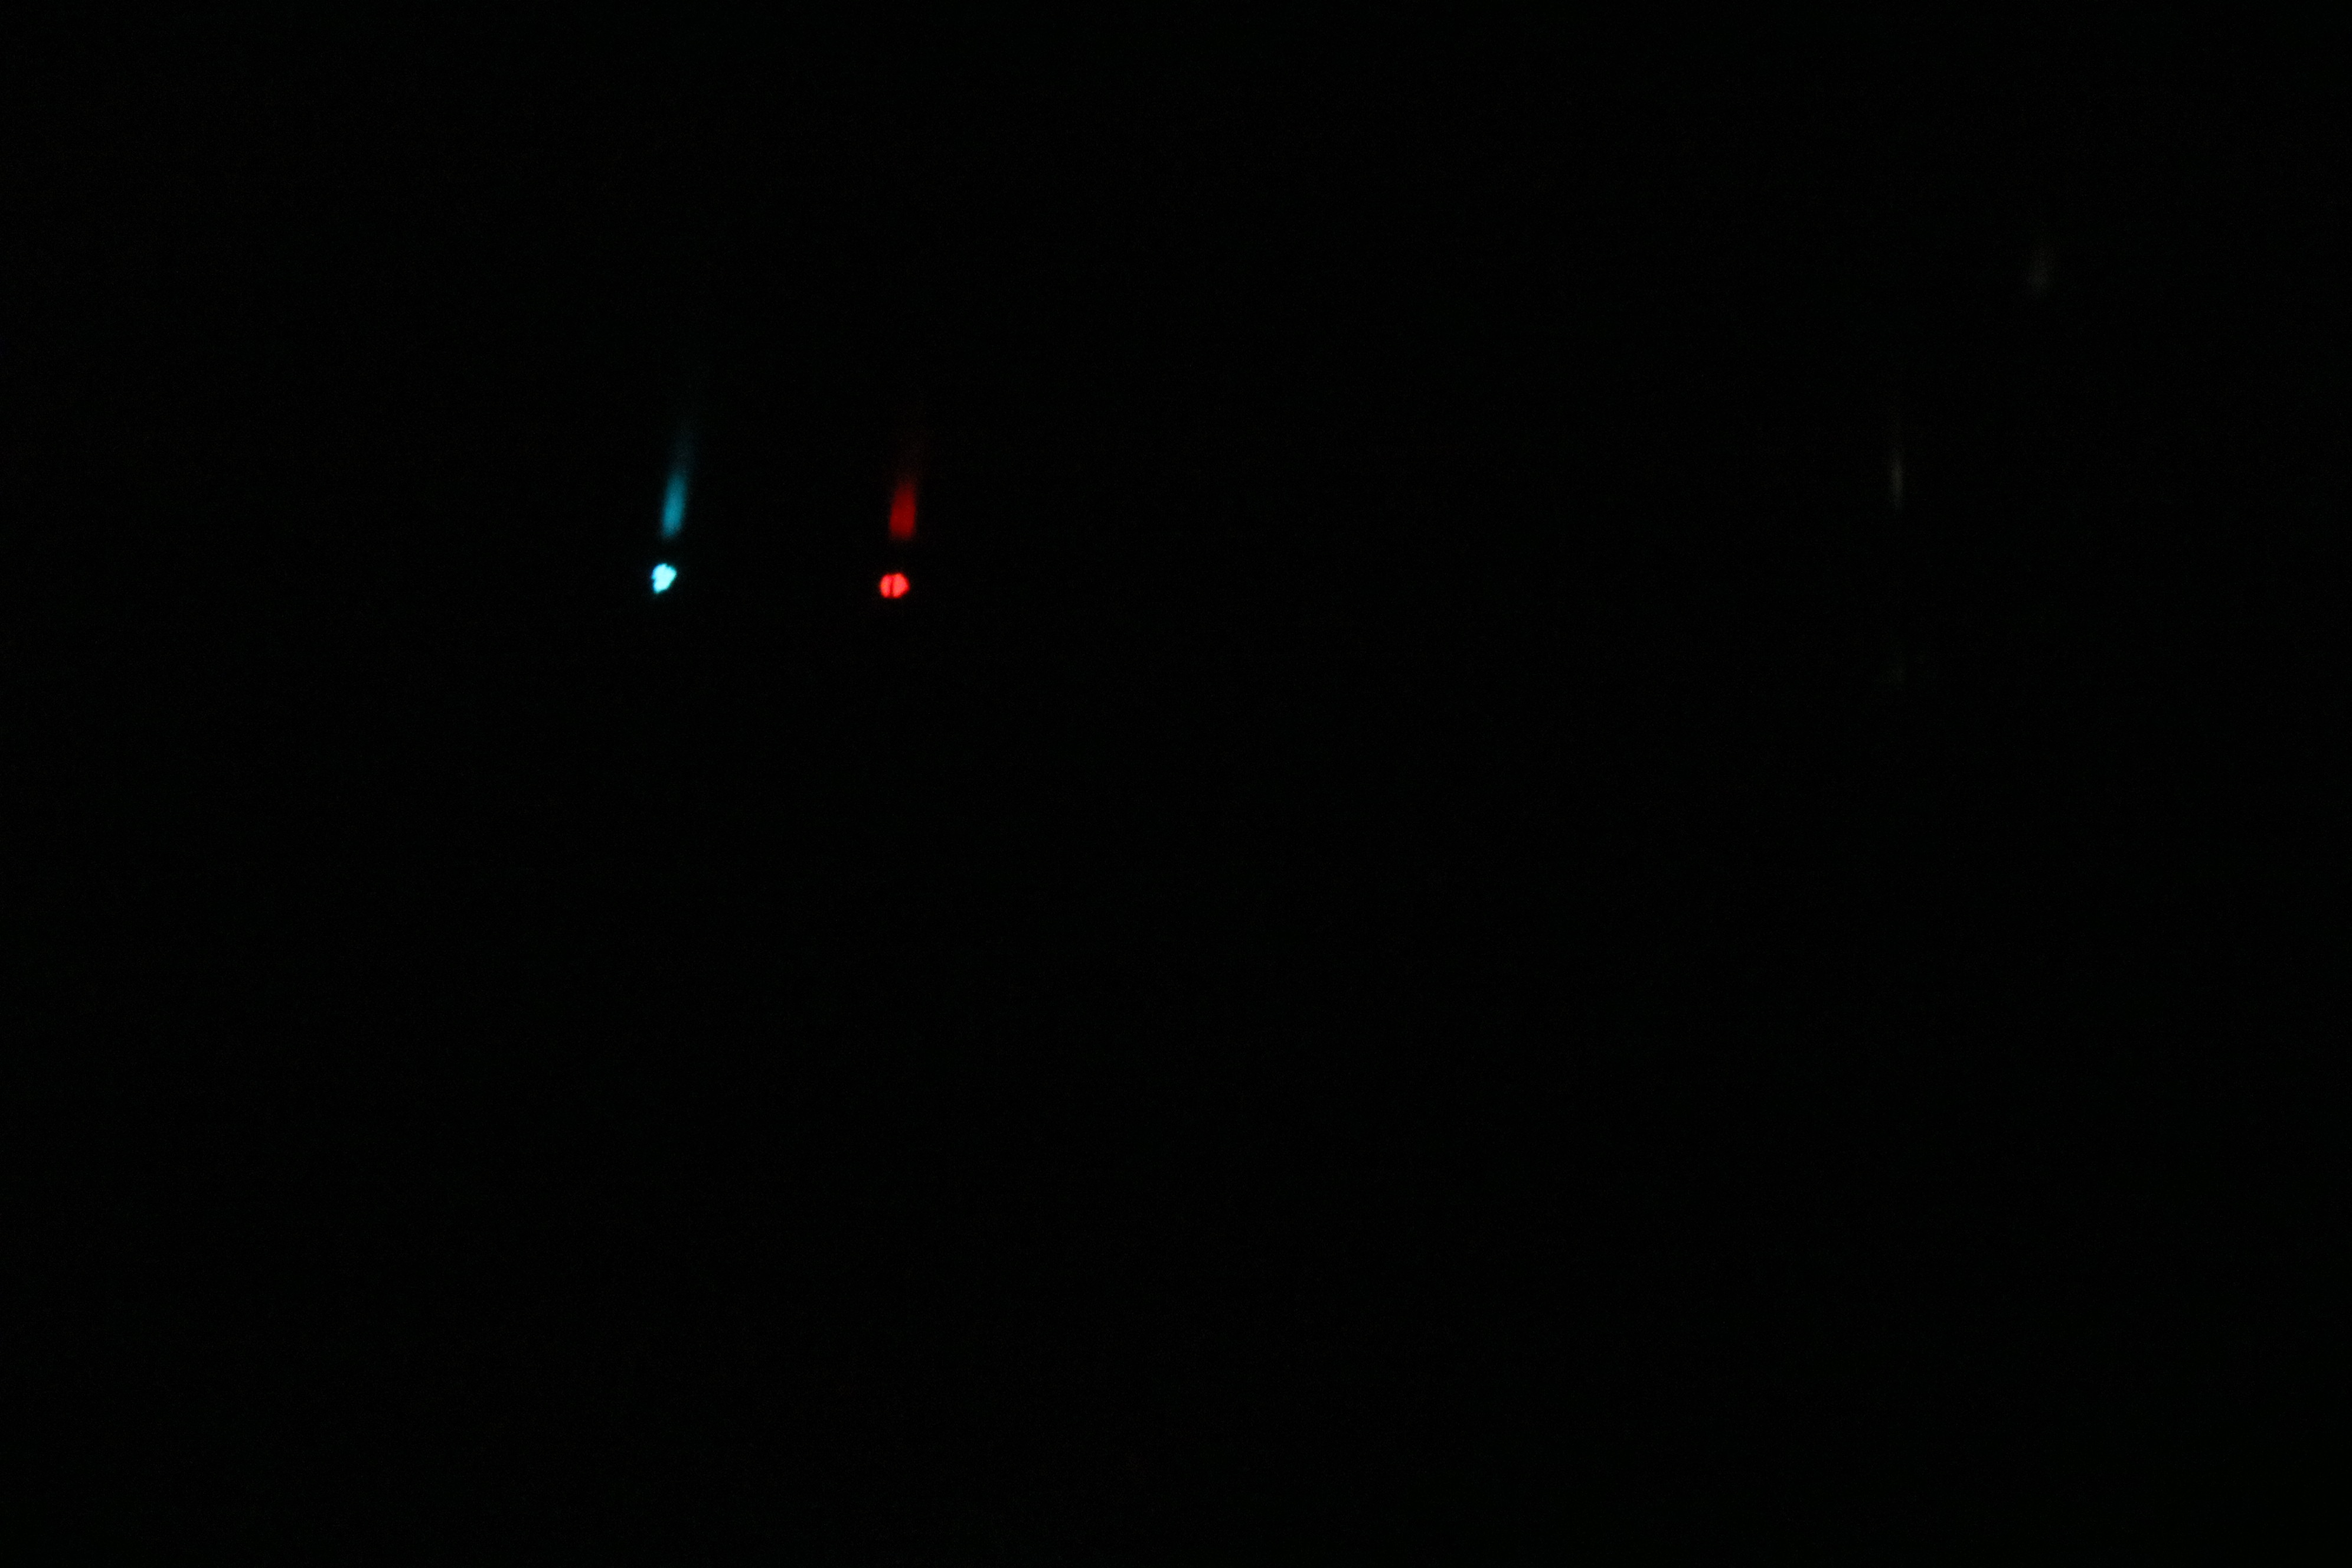
\includegraphics[width=.7\linewidth, height=1in]{z_68in.JPG}
		\caption{z=68 inches}
	\end{minipage}
	\begin{minipage}[b]{.5\linewidth}
		\centering
		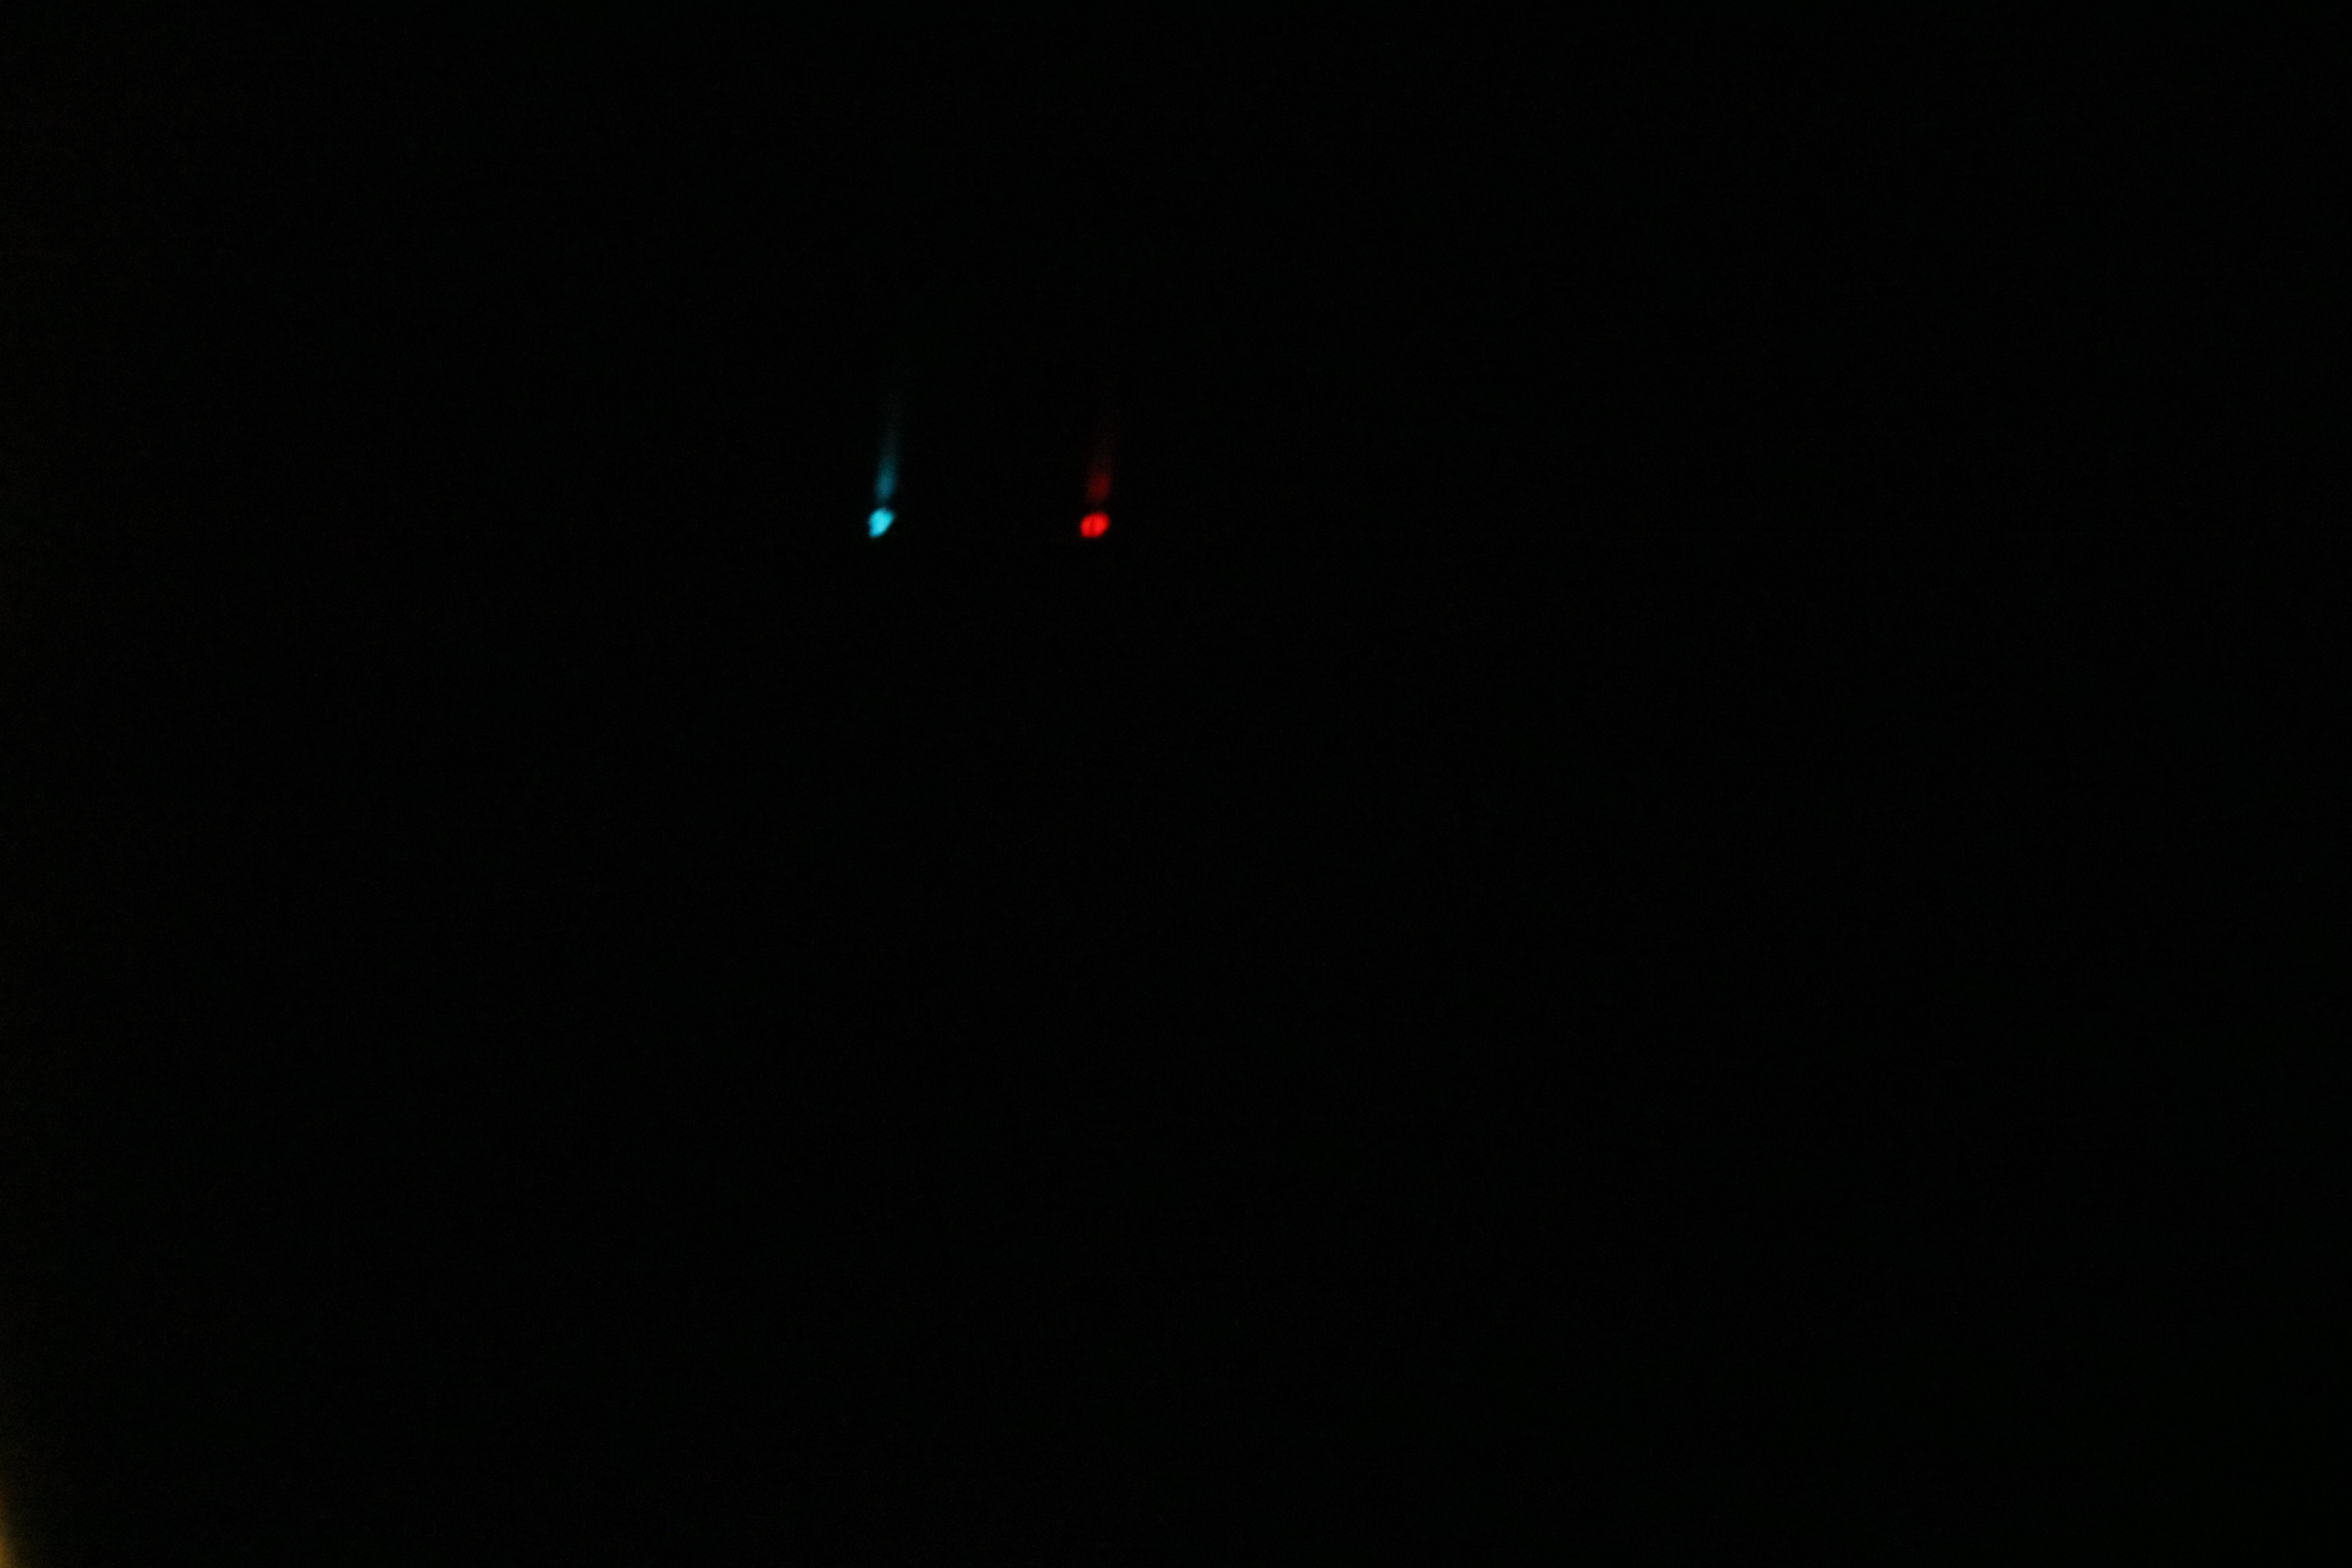
\includegraphics[width=.7\linewidth, height=1in]{z_85_take_2.JPG}
		\caption{z=85 inches}
	\end{minipage}
	\end{figure}
	
\newline lntuitively , as you go farther from the holes,ie. as $z$ increases, the rays should converge to a smaller $d$ value on the white paper , hence this is consistent with the graphs below since as z increases , $d$ decreases.From the scatter plots , it can be seen that generally as $d$ increases $z$ decreases and as $d$ decreases , $z$ increases both emperically and using the formula.
	
\begin{document}
\begin{figure}[H]
	\centering
	\begin{minipage}[b]{.5\linewidth}
		\centering
		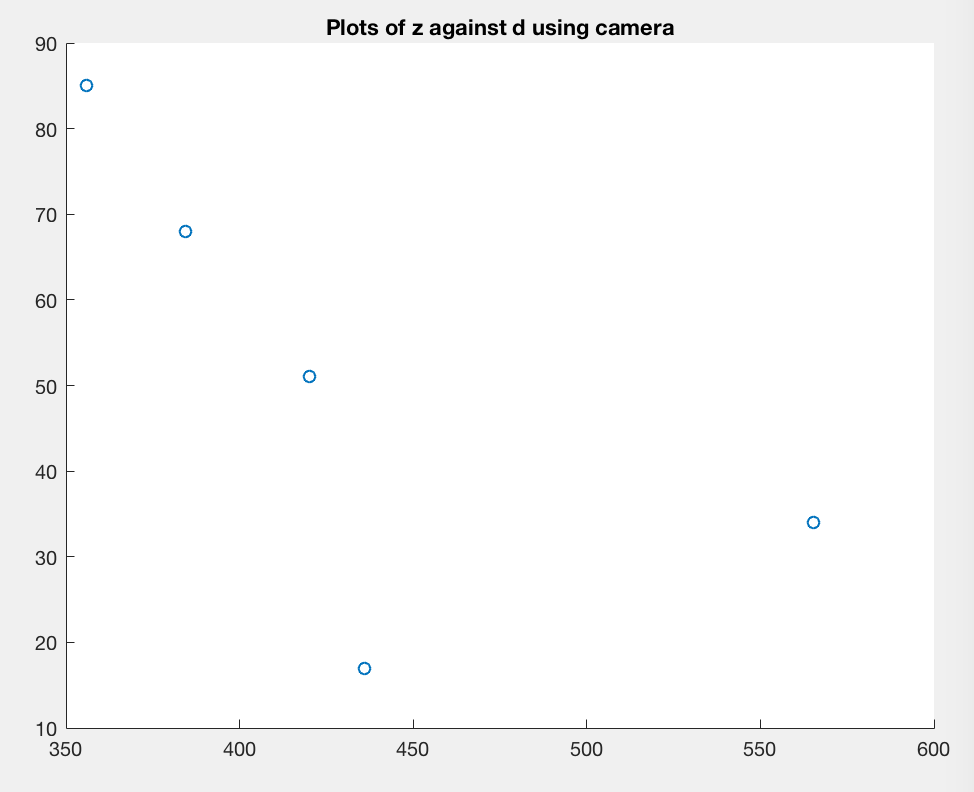
\includegraphics[width=2\linewidth, height=2in]{cam_plots}
		\caption{graph of z against d using camera images}
	\end{minipage}
	\begin{minipage}[b]{.5\linewidth}
		\centering
		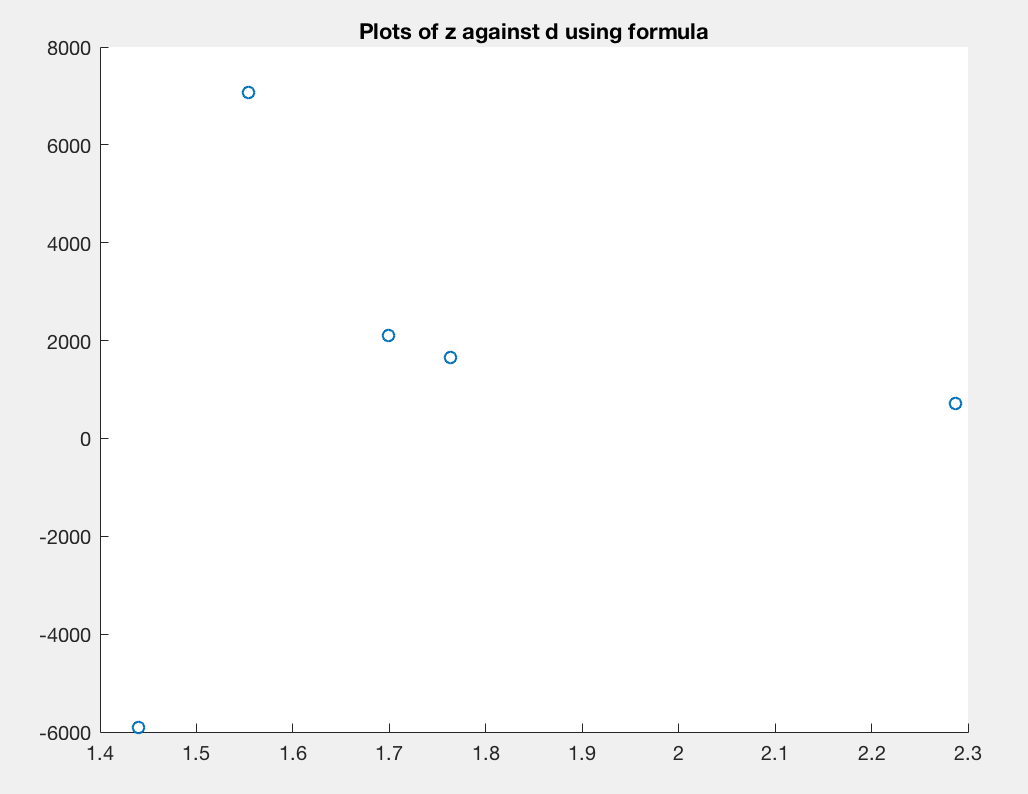
\includegraphics[width=2\linewidth, height=2in]{formula_plots}
		\caption{graph of z against d using pre-known d-values}
	\end{minipage}
\end{figure}

\end{document}